%% ============================================================================
%%  Transition-map contact mechanics on a neural coordinate atlas
%%  Target journal: Computer Methods in Applied Mechanics and Engineering (CMAME)
%%  Class: Springer svjour3 (matching the group's CMAME submission template)
%%
%%  Build:  latexmk -pdf main.tex
%%  Per-section "% code: <file::symbol>" comments tie each claim to the source.
%% ============================================================================
\documentclass{svjour3}                 % onecolumn (standard format)
\smartqed                               % flush-right qed marks

\usepackage{amsmath,amsfonts,amssymb}
\usepackage{newtxtext,newtxmath}        % Times-compatible text + math
\usepackage{bm}
\usepackage{xcolor}
\usepackage{graphicx}
\usepackage{booktabs}
\usepackage{multirow}
\usepackage{array}
\usepackage{upgreek}
\usepackage{placeins}
\usepackage{enumitem}
\usepackage{indentfirst}

\usepackage{tikz}
\usetikzlibrary{arrows.meta,calc,positioning,decorations.markings,fit,backgrounds,
  patterns,shapes.geometric,shapes.misc,angles,quotes}

\usepackage{natbib}
\setcitestyle{numbers,square,comma}

\usepackage[letterpaper,margin=3cm]{geometry}

\usepackage{lineno}
\linenumbers                            % line numbers for review submission

\journalname{Computer Methods in Applied Mechanics and Engineering}

%% --- notation macros (used throughout the section files) --------------------
\newcommand{\R}{\mathbb{R}}
\newcommand{\Sph}{\mathbb{S}}
\newcommand{\norm}[1]{\lVert#1\rVert}
\newcommand{\abs}[1]{\lvert#1\rvert}
\newcommand{\dhat}{\hat{\bm{d}}}
\newcommand{\nbf}{\bm{n}}
\newcommand{\tbf}{\bm{t}}
\newcommand{\xbf}{\bm{x}}
\newcommand{\ubf}{\bm{u}}
\newcommand{\fbf}{\bm{f}}
\newcommand{\vbf}{\bm{v}}
\newcommand{\gn}{g_{\scriptscriptstyle N}}
\newcommand{\tmap}{\tau_{AB}}
\newcommand{\map}[1]{\varphi_{#1}}
\newcommand{\pos}[1]{\langle #1\rangle_{+}}
\newcommand{\muapp}{\mu_{\mathrm{app}}}
\newcommand{\grad}{\nabla}
\newcommand{\code}[1]{\texttt{#1}}

\graphicspath{{../figures/}{figures/}}

\begin{document}

\title{Transition-map contact mechanics on a neural coordinate atlas:
resolving rough and non-convex geometry that the level set smooths}
\titlerunning{Transition-map contact on a neural atlas}

\author{WaiChing Sun}
\institute{WaiChing Sun \at
  Department of Civil Engineering and Engineering Mechanics, Columbia University,
  614 SW Mudd, 500 W 120th St, New York, NY 10027, USA \\
  \email{ws2414@columbia.edu}}

\date{Received: [DATE] / Accepted: [DATE]}

\maketitle

\begin{abstract}
We study contact between geometrically complex bodies and argue that the geometric representation, not
the constraint-enforcement scheme, is the dominant control on accuracy. Contact is posed as a
boundary-to-boundary chart map, the transition map, that composes the inverse of one body's boundary
chart with the other's; on a learned coordinate atlas this map delivers the gap, the surface normal, and
the active set directly, without an ambient level set. We build the atlas from Fourier-feature coordinate
charts, whose random-feature embedding defeats the spectral bias that smooths a neural signed-distance
function across sharp asperities and cusps. The neural level set is retained throughout as the compared
baseline, evaluated on the same meshes and tolerances. The method is verified against closed-form
solutions on a six-problem ladder, CV-1 through CV-6, spanning Hertz line contact, Cattaneo stick--slip,
the Brazilian disc, a nine-disc unit cell, a superformula boundary, and a Koch refinement ceiling, with
errors of a few percent or below. It is then validated on a real Inada-granite tensile fracture, where
dilation and apparent friction emerge from the resolved asperity geometry under plain Coulomb friction
with no imposed dilatancy law. The level set smooths the mean asperity slope from $19.4^\circ$ to
$12.5^\circ$ and under-predicts peak shear strength by $61\%$ on the granite joint, and under-predicts the
emergent dilatancy by $98\%$ on a synthetic rough block, while the chart reconstructs the surface to
$2.3~\mu$m against $107~\mu$m for the level set.
\keywords{computational contact mechanics \and coordinate atlas \and transition map \and
neural signed-distance function \and Fourier-feature charts \and rock-joint dilatancy}
\end{abstract}

\section{Introduction}\label{sec:intro}

\subsection{Geometry, not the force law, controls contact fidelity}\label{sec:intro-motivation}

A computational contact algorithm must answer two local questions about a query point $\xbf$ near a
body $X$. First, is $\xbf$ inside $X$, and by how much? This is the gap $\gn$. Second, which way is
out? This is the normal $\nbf$. We use the sign convention $\gn<0\Leftrightarrow$ penetration throughout.
Once these two quantities are produced, a mature library of enforcement schemes (penalty, augmented
Lagrangian, mortar, Nitsche) converts them into nodal forces \citep{wriggers2006computational,
laursen2002computational,kikuchi1988contact}. On smooth, convex bodies this division of labour is
benign. The gap and the normal are smooth functions of position, every scheme converges to the same
answer, and the discussion centres on constraint enforcement.

% code: solvers/contact/gap.py::evaluate_gap
On geometrically complex bodies the same division of labour breaks down. The gap and the normal are
no longer smooth, or even single-valued, so the \emph{geometric representation} from which they are read
becomes the dominant control on accuracy. A rock joint, a cusped cam lobe, a faceted aggregate, or a
self-similar fractal boundary all carry contact information at length scales an ambient field of fixed
capacity cannot store. The thesis of this paper is one sentence: \emph{on rough and non-convex
geometry the representation of the boundary, not the constraint-enforcement scheme, controls contact
fidelity.} We make this thesis precise and give it a method: contact read from a chart
\emph{transition map} on a learned coordinate atlas. We then measure it against the incumbent
representation on a verification ladder that runs from closed-form benchmarks to a real rock joint.

\subsection{The level set and its two intrinsic weaknesses}\label{sec:intro-levelset}

% code: solvers/contact/gap.py::evaluate_gap
The incumbent representation is the level set. For a body $A$ one stores a signed-distance function
$\phi_A:\R^d\to\R$, negative inside the body and increasingly represented by a neural network, and reads
the gap and the normal directly from the field. The gap is the field value at the query point, and the
outward normal is its normalized gradient:
\begin{equation}
  \gn(\xbf)=\phi_A(\xbf),\qquad
  \nbf(\xbf)=\frac{\grad\phi_A(\xbf)}{\norm{\grad\phi_A(\xbf)}},
  \label{eq:sdf-gap-intro}
\end{equation}
so a single automatic-differentiation call delivers both quantities at once
\citep{liu2020implicit,kolev2003level}. The economy of \eqref{eq:sdf-gap-intro} is the appeal of the
representation, and the source of its weaknesses. To make $\phi_A$ a true signed \emph{distance}, one
trains it with the eikonal penalty, which pushes the gradient toward unit norm everywhere:
\begin{equation}
  \mathcal{L}_{\mathrm{eik}}
  =\mathbb{E}_{\xbf\sim\Omega}\!\left[\big(\norm{\grad\phi_A(\xbf)}-1\big)^2\right],
  \label{eq:eikonal}
\end{equation}
where $\Omega$ is the sampling domain and the expectation averages the unit-gradient residual over it.
This penalty is combined with surface and normal-alignment losses on a boundary point cloud. We use the
level set throughout the paper \emph{only as the comparison baseline}. It is a fair and capable baseline,
not a strawman. On the geometry it can represent, it is exactly as accurate as the chart
(Section~\ref{sec:verif}).

The level set carries two weaknesses that are intrinsic to the representation rather than artefacts of
training, and both bear directly on contact:
\begin{enumerate}
  \item \textbf{Medial-axis non-smoothness.} The exact Euclidean signed distance is only $C^0$ on the
        medial axis, the locus equidistant from two or more boundary points, where the closest-point map
        is multivalued and $\grad\phi$ jumps. In a concavity the medial set reaches close to the
        surface, so the gradient normal of \eqref{eq:sdf-gap-intro} degrades precisely where a non-convex
        contact forms.
  \item \textbf{Spectral bias.} A coordinate multilayer perceptron learns low frequencies first and high
        frequencies slowly or never; its neural-tangent kernel is Laplace-like, with high-frequency
        power decaying \citep{rahaman2019spectral}. A fixed-capacity neural $\phi_A$ therefore low-passes
        cusps, asperities, and fine detail: it cannot represent a boundary sharper than its capacity
        ceiling, and it smooths the geometry that, on a rough joint, carries the strength.
\end{enumerate}
We measure both weaknesses, rather than merely assert them, in Sections~\ref{sec:verif}
and~\ref{sec:cv7}. The chart introduced next is built to avoid both: it stores one fewer
dimension, and it hands the network the high frequencies it would otherwise fail to learn.

\subsection{Related work}\label{sec:intro-related}

\paragraph{Signed-distance and closest-point contact.}
Reading a gap and a normal from an implicit field is established practice. \citet{kolev2003level} treat
the contact interface as the zero level set of one body's field restricted to the other; the
implicit-level-set material point method of \citet{liu2020implicit} reads the normal gap and contact
normal from a per-body signed-distance representation, and our force machinery reuses its normal-gap
form. The node-to-surface projection of \citet{zavarise1998segment} and \citet{fischer2005frictionless}
obtains a smooth, differentiable correspondence by closest-point projection without explicit facet
intersection, the same smoothness the implicit field provides. It returns only a \emph{single} foot,
however, which is the kinematic limitation the transition map removes (Section~\ref{sec:tmap}).

\paragraph{Neural implicit geometry, spectral bias, and Fourier features.}
Neural signed-distance and occupancy networks \citep{park2019deepsdf} and periodic-activation networks
\citep{sitzmann2020implicit} represent geometry implicitly with a fixed-capacity network, and inherit the
spectral bias characterized by \citet{rahaman2019spectral}: high-frequency detail is learned slowly or
not at all. The remedy we adopt is Fourier-feature input encoding \citep{tancik2020fourier}, which lifts
the input through a fixed bank of sinusoids and flattens the neural-tangent kernel to a tunable cutoff;
the same encoding underlies the positional encoding of neural radiance fields \citep{mildenhall2020nerf}.
We use Fourier features not to sharpen an ambient field but to sharpen a \emph{boundary} chart, which is
one dimension lower and therefore far easier to fit to a prescribed cutoff (Section~\ref{sec:fourier}).

\paragraph{Constraint enforcement.}
The forces that consume the gap and the normal are standard. We use penalty and augmented-Lagrangian
normal contact with regularized Coulomb friction \citep{wriggers2006computational,alart1991mixed,
simo1992augmented}, set against the mortar \citep{puso2004mortar} and Nitsche \citep{chouly2013nitsche}
families and the variational-inequality foundations of \citet{kikuchi1988contact} and
\citet{laursen2002computational}. These schemes are orthogonal to our contribution. Because every one of
them consumes only the gap, the normal, and the normal-force magnitude, the chart and the level set are
interchangeable at the force layer, and the geometry is the only thing we vary.

\paragraph{Rock-joint constitutive laws.}
The validation problem is the direct shear of a rough rock joint, for which a mature constitutive
literature supplies the closed-form anchor and the physical interpretation of the measured numbers. The
bilinear law of \citet{patton1966multiple} gives the apparent friction angle of a regularly serrated
joint as $\phi_b+i$, with $\phi_b$ the basic friction angle and $i$ the asperity inclination; the
empirical model of \citet{barton1977shear} and the review of \citet{barton1990review} extend this to
natural roughness; the asperity-degradation model of \citet{plesha1987constitutive} and the joint element
of \citet{goodman1976methods} supply the interface kinematics for cyclic shear. In our framework the
dilatancy and the apparent friction are not imposed through such a law. They \emph{emerge} from the
resolved asperity geometry, and the Patton law is the reference these emergent quantities are checked
against.

\subsection{Contributions}\label{sec:intro-contributions}

\begin{enumerate}
  \item \textbf{A transition-map contact detector.} We read contact from the boundary-to-boundary chart
        map $\tmap=\map{B}^{-1}\circ\map{A}$ between two bodies of a learned atlas, rather than from an
        ambient field. The detector returns a matched, conservative gap--normal pair, in which the normal
        is the gradient of the gap, so the penalty force is the exact gradient of a potential. A
        boundary scan then enumerates \emph{every} disjoint contact arc, where a closest-point projection
        returns one foot. This is the paper's central method (Section~\ref{sec:tmap}).
  \item \textbf{Fourier-feature coordinate charts with a verify-first protocol.} We instantiate the chart
        in three families: a radial height field $\rho_\theta$ on the sphere of directions, an open
        graph height field $h_\theta$, and a boundary-fitted decoder $D_\theta$ inverted by Newton
        iteration. Each is encoded with a Fourier-feature bank sized to the geometry's resolvable
        bandwidth. We verify every chart against a closed form or a manufactured solution before we use
        it to drive contact (Section~\ref{sec:fourier}).
  \item \textbf{A characterization of when the chart beats the level set.} We show that the radial
        inverse-chart gap is conservative-large but \emph{sign-exact},
        $g_{\mathrm{rad}}=g_\perp/\cos\alpha+O(g^2)$ with $\alpha$ the ray-to-normal angle, so the
        chart's active set matches the true level set's on star-shaped bodies; and we give the
        complementary spectral-bias argument that a $(d{-}1)$-dimensional boundary function fits a
        prescribed cutoff where a $d$-dimensional ambient field cannot
        (Sections~\ref{sec:tmap}--\ref{sec:fourier}).
  \item \textbf{A verification ladder CV-1 through CV-6 and a real-joint validation CV-7.} We place the
        chart and the level set on the same problems: the convex, superposable closed forms
        (CV-1 Hertz, CV-2 Cattaneo--Mindlin, CV-3 Brazilian, CV-4 nine-disc), where they are equivalent
        and the chart buys nothing; the cusped non-convex superformula (CV-5) and the
        self-similar Koch fractal (CV-6), where the chart measurably wins; and the direct shear of a real
        Inada-granite fracture (CV-7), where the resolved asperities drive emergent dilatancy and strength
        (Sections~\ref{sec:verif}--\ref{sec:cv7}).
  \item \textbf{Embedding in chart-FEM and MPM.} The detector is an opt-in geometric oracle: it composes
        with the existing chart-based finite-element and material-point solvers without modifying the
        force laws, the broad-phase culler, or the time integrator (Section~\ref{sec:form}).
\end{enumerate}

% code: benchmarks/contact/cv_numerical/cv7_transition_map_contact.py
A handful of measurements anchor these claims. On the cusped superformula (CV-5) the neural radial chart
attains a gap error of $3.8\times10^{-3}L$ and a $0.42^\circ$ median normal-angle error, against
$8\times10^{-3}L$ and a degraded normal for the neural level set, and it drives the cam dynamics to a
$0.04\%$ trajectory match. On the real Inada joint (CV-7) the height chart reconstructs the surface to
$2.3\,\mu$m where an ambient neural level set reaches only $107\,\mu$m; the level set smooths the mean
asperity angle from $19.4^\circ$ to $12.5^\circ$ and, through the Patton law, under-predicts peak shear
strength by $61\%$. On a band-limited surface carried by a trained decoder the level set under-predicts
emergent dilatancy by $98\%$ and strength by $35\%$, while the transition-map detector in the contact
loop agrees with the analytic active set $98.9\%$ of the time, against $95.8\%$ for the level set
(Sections~\ref{sec:verif}--\ref{sec:cv7}).

\subsection{Notation and organization}\label{sec:intro-notation}

Bodies are labelled $A,B,\dots$; the interior of body $X$ is $\Omega_X\subset\R^d$ ($d=2,3$) and its
boundary $\partial\Omega_X$. A \emph{chart} is a parametrization of a body's boundary,
$\map{X}:\Theta_X\to\partial\Omega_X$; a \emph{level set} is an ambient scalar field $\phi_X:\R^d\to\R$
whose zero set is $\partial\Omega_X$. The transition map between two charted bodies is
$\tmap=\map{B}^{-1}\circ\map{A}$. We write the Macaulay bracket $\pos{z}=\max(0,z)$ and keep the sign
convention $\gn<0\Leftrightarrow$ penetration. The apparent friction coefficient measured from a contact
run is $\muapp$, to be compared against the Patton value $\tan(\phi_b+i)$.

The remainder of the paper is organized as follows. Section~\ref{sec:tmap} defines the
transition map, derives the matched gap--normal pair and the multi-arc enumeration, and states the
$1/\cos\alpha$ radial-gap bound with its active-set equivalence. Section~\ref{sec:fourier} develops the
Fourier-feature charts and the spectral-bias argument that they defeat. Section~\ref{sec:form}
gives the force laws and the embedding in chart-FEM and MPM. Section~\ref{sec:verif} reports the
closed-form ladder CV-1 through CV-6. Section~\ref{sec:cv7} reports the real-joint validation
CV-7. Section~\ref{sec:disc} states the scope, preconditions, and limitations, and
Section~\ref{sec:concl} concludes.

\section{The transition map for contact}\label{sec:tmap}

Every contact algorithm answers two questions about a query point $\xbf$ that sits near a body $X$. Is
$\xbf$ inside $X$, and if so by how much? This signed depth is the \emph{gap}. Which way is outward? This
direction is the \emph{normal}. The neural-atlas framework answers both questions from one of two ways of
describing the body. The thesis of this paper is that the description, not the scheme that enforces the
contact constraint, controls accuracy on geometrically hard contact.

A few conventions fix the signs and the notation we use throughout. The gap is negative when the point
penetrates the body: $\gn<0\Leftrightarrow$ penetration, so an interior point reads a negative gap and two
surfaces that overlap read a negative gap. The Macaulay bracket $\pos{z}=\max(0,z)$ keeps only the
positive part of its argument and so isolates the penetrating cases. We label bodies $A,B,\dots$; a body's
interior is the open region $\Omega_X\subset\R^d$ in $d=2$ or $3$ dimensions, and its boundary is the
surface $\partial\Omega_X$. We describe that boundary in two ways. A \emph{chart} parametrizes
the boundary directly, $\map{X}:\Theta_X\to\partial\Omega_X$, sending a parameter $\theta\in\Theta_X$ to
the surface point it labels. A \emph{level set} instead fills all of space with a scalar field
$\phi_X:\R^d\to\R$ whose zero crossing is the boundary $\partial\Omega_X$. The next subsection compares the
two.

\subsection{Two ways to describe a body}\label{sec:tmap:two}

\subsubsection{The ambient level set}

The classical description stores a signed-distance function, a scalar field over all of space whose value
is the distance to the surface, negative inside and positive outside. For body $A$ we train a neural
network $\phi_A:\R^d\to\R$ to approximate this field, and we read the gap and the outward normal from the
field and its gradient. The gap is the field value, and the normal is the field's gradient made into a
unit vector.
%
\begin{equation}\label{eq:sdf-gap}
\gn^A(\xbf)=\phi_A(\xbf),\qquad
\nbf_A(\xbf)=\frac{\grad\phi_A(\xbf)}{\norm{\grad\phi_A(\xbf)}}.
\end{equation}
%
Here $\grad\phi_A$ is the spatial gradient of the field and $\norm{\cdot}$ is the Euclidean norm, so both
the gap and the normal come from one automatic-differentiation call. We train the network to behave like a
true distance through the Eikonal penalty $\mathbb E_{\xbf}\big[(\norm{\grad\phi}-1)^2\big]$, which drives
the gradient to unit length, together with a surface loss, a normal-alignment loss, and sign-anchor terms
\citep{liu2020implicit,park2019deepsdf}; the architecture is a $\tanh$ multilayer perceptron.

The level set fails on hard geometry in two ways. Both are built into the description rather than being
fixable implementation defects. The first is the medial axis. The exact Euclidean signed distance is only
$C^0$ on the locus of points equidistant from two or more boundary points, because there the nearest-point
map is multivalued and the gradient $\grad\phi$ jumps. In a concavity this medial set reaches close to the
surface, so the gradient normal degrades exactly where a nonconvex contact happens
\citep{kolev2003level}. The second is spectral bias. A coordinate network learns low frequencies first and
high frequencies slowly or never, because its neural-tangent kernel is Laplace-like
\citep{rahaman2019spectral}. A network $\phi$ of fixed capacity therefore smooths cusps, asperities, and
fine detail; it cannot represent a boundary sharper than its capacity ceiling.
Section~\ref{sec:fourier} makes this quantitative.

\subsubsection{The boundary chart}

The alternative stores only the boundary, written as a function of the boundary's own parameter. Three
chart families appear in this work, in order of increasing generality. The \emph{radial chart}
$\rho_X:\Sph^{d-1}\to\R^+$ is a height field on the sphere of directions: for each unit direction it
records how far the surface lies from the center. It works for star-shaped bodies, those seen entirely
from one interior point. With center $c_X$ and orientation $Q_X$ (the body axes as columns), the boundary
point in direction $\hat\ubf$ is $\map{X}(\hat\ubf)=c_X+Q_X\,\rho_X(\hat\ubf)\,\hat\ubf$. The \emph{height
chart} $h_X:\mathcal D\to\R$ over an open parameter domain $\mathcal D$ is the graph $z=h(x)$ of a
single-valued rough surface, such as one face of a rock joint. The \emph{decoder chart}
$D_X:\bm\xi\mapsto\xbf$ is a boundary-fitted volumetric map for general, possibly non-star-shaped geometry,
inverted by Newton iteration.

A chart costs less to fit than a level set, for a simple reason. The radius or
height function lives in one dimension fewer than the ambient field, models no interior, and carries no
medial axis. The price is a precondition that the body must meet (star-shapedness for radial charts,
single-valuedness for height charts) and a gap measured along a ray rather than perpendicular to the
surface (Section~\ref{sec:tmap:bias}). The payoff is fidelity, because a $(d{-}1)$-dimensional boundary
function is far easier to fit sharply than a $d$-dimensional ambient field.
Figure~\ref{fig:tm-levelset-vs-chart} contrasts the two descriptions.

\begin{figure}
\centering
\resizebox{\linewidth}{!}{%
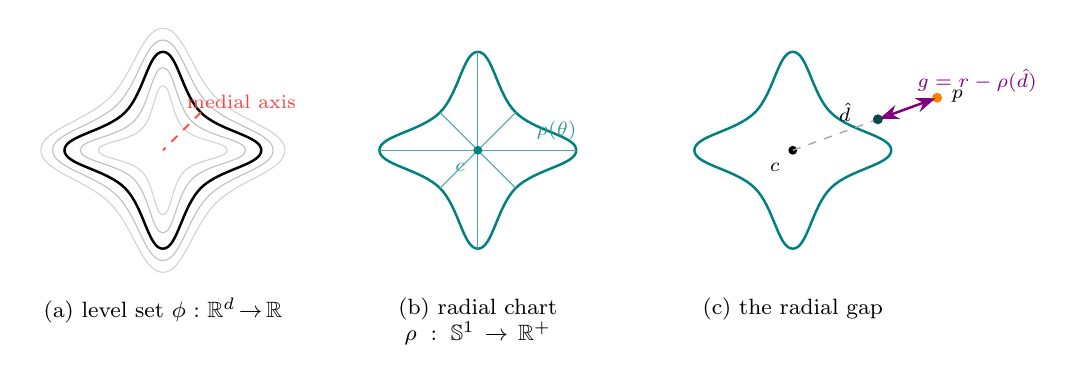
\begin{tikzpicture}[font=\footnotesize,>=Stealth,line join=round,
  starpts/.style={}]

  % ===== reusable star coordinates (concave notches) =====
  % defined relative to each panel origin via shifts

  %% ---------------------------------------------------------------
  %% PANEL (a): level set
  %% ---------------------------------------------------------------
  \begin{scope}[shift={(0,0)}]
    % nested OUTER level-set contours (fainter)
    \draw[gray!35,line width=0.4pt] plot[smooth cycle,tension=0.7]
      coordinates {(0:1.55)(45:0.95)(90:1.55)(135:0.95)(180:1.55)(225:0.95)(270:1.55)(315:0.95)};
    \draw[gray!50,line width=0.4pt] plot[smooth cycle,tension=0.7]
      coordinates {(0:1.4)(45:0.82)(90:1.4)(135:0.82)(180:1.4)(225:0.82)(270:1.4)(315:0.82)};
    % the body boundary (zero level set)
    \draw[black,line width=0.9pt] plot[smooth cycle,tension=0.7]
      coordinates {(0:1.25)(45:0.68)(90:1.25)(135:0.68)(180:1.25)(225:0.68)(270:1.25)(315:0.68)};
    % nested INNER contours (fainter)
    \draw[gray!50,line width=0.4pt] plot[smooth cycle,tension=0.7]
      coordinates {(0:1.05)(45:0.52)(90:1.05)(135:0.52)(180:1.05)(225:0.52)(270:1.05)(315:0.52)};
    \draw[gray!35,line width=0.4pt] plot[smooth cycle,tension=0.7]
      coordinates {(0:0.82)(45:0.38)(90:0.82)(135:0.38)(180:0.82)(225:0.38)(270:0.82)(315:0.38)};
    % medial axis: dashed line from a concave notch toward interior
    \draw[red!70,dashed,line width=0.7pt] (45:0.68) -- (0,0);
    \node[red!75,font=\scriptsize,anchor=west] at (0.18,0.62) {medial axis};
    % title
    \node[anchor=north,text width=3.2cm,align=center] at (0,-1.75)
      {(a) level set $\phi:\mathbb{R}^d\!\to\!\mathbb{R}$};
  \end{scope}

  %% ---------------------------------------------------------------
  %% PANEL (b): radial chart
  %% ---------------------------------------------------------------
  \begin{scope}[shift={(4.0,0)}]
    % body boundary in teal
    \draw[teal,line width=0.9pt] plot[smooth cycle,tension=0.7]
      coordinates {(0:1.25)(45:0.68)(90:1.25)(135:0.68)(180:1.25)(225:0.68)(270:1.25)(315:0.68)};
    % 8 thin rays center -> boundary
    \draw[teal!70,line width=0.4pt] (0,0)--(0:1.25);
    \draw[teal!70,line width=0.4pt] (0,0)--(45:0.68);
    \draw[teal!70,line width=0.4pt] (0,0)--(90:1.25);
    \draw[teal!70,line width=0.4pt] (0,0)--(135:0.68);
    \draw[teal!70,line width=0.4pt] (0,0)--(180:1.25);
    \draw[teal!70,line width=0.4pt] (0,0)--(225:0.68);
    \draw[teal!70,line width=0.4pt] (0,0)--(270:1.25);
    \draw[teal!70,line width=0.4pt] (0,0)--(315:0.68);
    % center dot
    \fill[teal] (0,0) circle (1.6pt);
    \node[teal!80,font=\scriptsize,anchor=north east] at (-0.04,-0.04) {$c$};
    % a sample angle label
    \node[teal!80,font=\scriptsize] at (0:1.0) [above] {$\rho(\theta)$};
    % title
    \node[anchor=north,text width=3.2cm,align=center] at (0,-1.75)
      {(b) radial chart $\rho:\mathbb{S}^1\!\to\!\mathbb{R}^{+}$};
  \end{scope}

  %% ---------------------------------------------------------------
  %% PANEL (c): the radial gap
  %% ---------------------------------------------------------------
  \begin{scope}[shift={(8.0,0)}]
    % body boundary
    \draw[teal,line width=0.9pt] plot[smooth cycle,tension=0.7]
      coordinates {(0:1.25)(45:0.68)(90:1.25)(135:0.68)(180:1.25)(225:0.68)(270:1.25)(315:0.68)};
    % center dot c
    \fill[black] (0,0) circle (1.6pt);
    \node[font=\scriptsize,anchor=north east] at (-0.04,-0.04) {$c$};
    % exterior point p along ~20 deg ray, beyond boundary
    \coordinate (P) at (20:1.95);
    % foot where ray meets boundary (green) ~ rho at 20deg
    \coordinate (F) at (20:1.15);
    % the ray c -> p
    \draw[gray!70,line width=0.5pt,dashed] (0,0)--(P);
    % unit direction marker hat d
    \node[font=\scriptsize,anchor=south] at (20:0.7) {$\hat{d}$};
    % foot dot (green)
    \fill[teal!60!black] (F) circle (1.8pt);
    % exterior point p
    \fill[orange] (P) circle (1.8pt);
    \node[font=\scriptsize,anchor=west] at ($(P)+(0.06,0.02)$) {$p$};
    % violet double arrow foot -> p  (the gap)
    \draw[violet,line width=0.9pt,<->] ($(F)+(20:0.02)$) -- ($(P)-(20:0.02)$);
    \node[violet,font=\scriptsize,anchor=south west] at ($(F)!0.5!(P)+(0,0.08)$)
      {$g=r-\rho(\hat{d})$};
    % title
    \node[anchor=north,text width=3.2cm,align=center] at (0,-1.75)
      {(c) the radial gap};
  \end{scope}

\end{tikzpicture}%
}
\caption{Two representations of the same star-shaped body. (a) The ambient level set
$\phi:\R^d\to\R$ fills all of space; its zero set is the boundary, but it carries a medial axis in the
interior where $\grad\phi$ is non-smooth, and a fixed-capacity neural $\phi$ low-passes sharp features.
(b) The radial boundary chart $\rho:\Sph^{1}\to\R^+$ stores only the boundary as a height field on the
circle of directions, with no ambient field and no medial axis. (c) The gap is read along the ray from
the center, $\gn=r-\rho(\dhat)$, with the matched normal $\grad_d F=\dhat-\grad_S\rho/r$.}
\label{fig:tm-levelset-vs-chart}
\end{figure}

\subsection{The transition map and why it detects contact}\label{sec:tmap:def}

\subsubsection{The idea before the formula}

Here is the central construction in one sentence. Take a point on body $A$'s surface and ask where that
point lands on body $B$'s surface. The transition map is the rule that answers, carrying every surface
point of $A$ to its counterpart on $B$. Two charts make this possible: each surface point of $A$ is named
by a parameter $\theta_A$, each surface point of $B$ by a parameter $\psi_B$, and the transition map turns
the first name into the second. It does so in two steps. First push the $A$-point into physical space with
$A$'s chart, then invert $B$'s chart to read off the $B$-parameter at that location.
%
\begin{equation}\label{eq:tmap-def}
\tmap:\ \theta_A\ \longmapsto\ \psi_B=\big(\map{B}^{-1}\circ\map{A}\big)(\theta_A).
\end{equation}
%
Reading the formula left to right: $\map{A}$ takes the parameter $\theta_A$ to the physical point
$\xbf=\map{A}(\theta_A)$ on $A$, and $\map{B}^{-1}$ takes that physical point back to the matching surface
parameter $\psi_B$ on $B$. The name is the standard one from differential geometry, where a transition map
is the change of coordinates $\map{B}^{-1}\circ\map{A}$ between two charts of an atlas; we apply it across
two bodies to read their contact correspondence. Figure~\ref{fig:tm-concept} illustrates the construction.

Once the correspondence is known, the contact normal follows from the chart's own geometry rather than
from a signed-distance gradient. Two tangent vectors span the surface at the contact point, and their
cross product points out of it. Normalizing that cross product gives the unit normal.
%
\begin{equation}\label{eq:jacobian-normal}
\nbf=\frac{\tbf_1\times\tbf_2}{\norm{\tbf_1\times\tbf_2}},\qquad
\tbf_\alpha=\frac{\partial\map{A}}{\partial\xi^\alpha},
\end{equation}
%
Here $\tbf_\alpha$ is the surface tangent obtained by differentiating the chart $\map{A}$ along its
parameter direction $\xi^\alpha$, and the normalized cross product $\nbf$ is the outward unit normal. The
undeformed normal gap is then the chart form of the implicit level-set MPM normal gap
\citep{liu2020implicit}, $g_{n0}=(\map{}^{(j)}-\map{}^{(i)})\cdot\nbf$, the projection of the
surface-to-surface offset onto that normal.

\begin{figure}
\centering
\resizebox{\linewidth}{!}{%
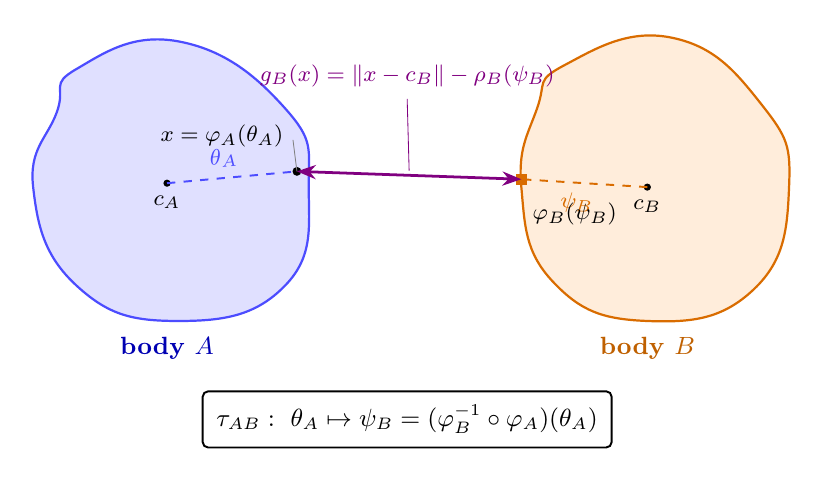
\begin{tikzpicture}[font=\footnotesize,>={Stealth[length=2.4mm]}]
  \fill[blue!12,draw=blue!70,line width=0.8pt]
    plot[smooth cycle,tension=0.8] coordinates
    {(-1.7,1.5) (-0.4,1.85) (0.95,1.0) (1.25,0.0) (0.95,-1.25)
     (-0.4,-1.7) (-1.7,-1.25) (-2.25,0.0) (-1.95,0.95)};
  \fill[orange!14,draw=orange!85!black,line width=0.8pt]
    plot[smooth cycle,tension=0.8] coordinates
    {(4.5,1.55) (5.85,1.9) (7.0,1.05) (7.35,0.0) (6.9,-1.3)
     (5.55,-1.7) (4.35,-1.2) (3.95,0.0) (4.15,1.0)};
  \coordinate (cA) at (-0.55,0.05);
  \coordinate (cB) at (5.55,0.0);
  \fill (cA) circle (1.3pt) node[below=1pt]{$c_A$};
  \fill (cB) circle (1.3pt) node[below=1pt]{$c_B$};
  \coordinate (x) at (1.1,0.2);
  \coordinate (foot) at (3.95,0.1);
  % rays
  \draw[blue!70,dashed,line width=0.7pt] (cA) -- (x) node[pos=0.45,above,sloped]{$\theta_A$};
  \draw[orange!85!black,dashed,line width=0.7pt] (cB) -- (foot) node[pos=0.55,below,sloped]{$\psi_B$};
  \fill (x) circle (1.6pt);
  \fill[orange!85!black] ($(foot)+(-0.07,-0.07)$) rectangle ($(foot)+(0.07,0.07)$);
  % gap arrow (long, between separated bodies)
  \draw[violet,line width=1pt,<->] (x) -- (foot);
  % spread labels: x-label up-left, gap formula high, foot-label down-right
  \node[anchor=east] at ($(x)+(-0.05,0.45)$) {$x=\varphi_A(\theta_A)$};
  \draw[gray,line width=0.3pt] ($(x)+(-0.05,0.40)$) -- (x);
  \node[violet,anchor=south] at (2.5,1.15) {$g_B(x)=\|x-c_B\|-\rho_B(\psi_B)$};
  \draw[violet,line width=0.3pt] (2.5,1.12) -- ($(x)!0.5!(foot)+(0,0.06)$);
  \node[anchor=north west] at ($(foot)+(0.02,-0.18)$) {$\varphi_B(\psi_B)$};
  % body labels + boxed map
  \node[font=\small\bfseries,blue!70!black] at (-0.55,-2.05) {body $A$};
  \node[font=\small\bfseries,orange!75!black] at (5.55,-2.05) {body $B$};
  \node[draw=black,line width=0.7pt,rounded corners=2pt,inner sep=5pt,font=\small]
    at (2.5,-2.95) {$\tau_{AB}:\ \theta_A\mapsto\psi_B=(\varphi_B^{-1}\circ\varphi_A)(\theta_A)$};
\end{tikzpicture}%
}
\caption{The transition map $\tmap=\map{B}^{-1}\circ\map{A}$. A boundary point $\xbf=\map{A}(\theta_A)$ of
body $A$ is taken into physical space, then $B$'s chart is inverted along the ray from $c_B$ to give
$\psi_B$ and the foot $\map{B}(\psi_B)$. The signed gap $\gn^B(\xbf)=\norm{\xbf-c_B}-\rho_B(\psi_B)$ falls
out of the inversion; no ambient field is evaluated.}
\label{fig:tm-concept}
\end{figure}

\subsubsection{Detection needs no ambient field}

% code: solvers/contact/chart_gap.py::evaluate_gap_chart ; solvers/contact/supershape.py::radial_gap
Detection asks only for a signed gap and an outward normal at a query point, and neither requires an
ambient field. Given $B$'s chart, three steps suffice: express the query point $\xbf$ in $B$'s local
coordinates, invert the chart to find the boundary parameter that the point points toward, and compare the
two radii. For a star-shaped body all three collapse to almost nothing: the inversion is a closed-form
direction, and the comparison is a single radius subtraction. We first form
the body-frame coordinate $\bm d=Q_B^\top(\xbf-c_B)$, which re-expresses the offset from $B$'s center in
$B$'s own axes, then split it into a direction and a length.
%
\begin{equation}\label{eq:radial-gap}
\dhat=\frac{Q_B^\top(\xbf-c_B)}{\norm{Q_B^\top(\xbf-c_B)}},\qquad
\gn^B(\xbf)=\underbrace{\norm{Q_B^\top(\xbf-c_B)}}_{r}-\rho_B(\dhat),
\end{equation}
%
Here $\dhat$ is the unit direction from $B$'s center to the query point, $r$ is the distance from the
center to the point, and $\rho_B(\dhat)$ is the chart's surface radius in that direction; the gap is the
point's radius minus the surface's radius. This gap is globally single-valued and $C^1$ wherever $\rho_B$
is, and it is negative exactly when the point lies inside. This is the level set turned inside out. A
signed-distance function answers ``how far is the nearest surface, in any direction'' by storing a field
over all of $\R^d$; the transition map answers ``which point of $B$'s boundary does this point correspond
to, and is it inside'' by storing only $\partial\Omega_B$ and inverting. On star-shaped and single-valued
geometry the second is both cheaper to store and sharper to fit.

In two dimensions the radial chart can carry an analytic radius, the Gielis superformula, which generates
a wide family of closed boundaries from a few parameters.
%
\begin{equation}\label{eq:superformula-chart}
\rho(\theta)=\Big(\big\lvert\tfrac1a\cos\tfrac{m\theta}{4}\big\rvert^{n_2}
+\big\lvert\tfrac1b\sin\tfrac{m\theta}{4}\big\rvert^{n_3}\Big)^{-1/n_1},
\end{equation}
%
Here $\theta$ is the polar angle, $m$ sets the number of lobes, and $a,b,n_1,n_2,n_3$ shape the lobes; the
inverse chart is simply $\theta=\angle\,Q_B^\top(\xbf-c_B)$, the angle of the body-frame offset, evaluated
by \code{atan2} \citep{gielis2003generic}. The analytic radius and a trained neural radius feed the
identical gap expression~\eqref{eq:radial-gap}: the evaluator itself is validated against the closed-form
gap to $10^{-10}$ on a self-test, and the trained neural radius reproduces the analytic gap to
$3.8\times10^{-3}L$ on the cusped superformula (Section~\ref{sec:verif}), so the neural chart is a drop-in
replacement for the analytic one.

\subsection{The matched conservative normal}\label{sec:tmap:matched}

One detail decides whether the contact forces conserve energy: the normal we return with the gap must be
the gradient of that gap. Only then is the penalty force the gradient of a potential, so that the work it
does is path-independent and nothing leaks. Differentiating the radial gap $F(\xbf)=r-\rho(\dhat)$ asks
for the gradient of $\rho$ with respect to direction, but that raw gradient is not what we want, because
$\rho$ is a function of a \emph{unit} vector. Moving along the direction $\dhat$ would change its length,
and $\rho$ does not respond to a length change. The raw gradient therefore carries a spurious
radial component that we must remove. We remove it by projecting onto the plane tangent to the direction
sphere.
%
\begin{equation}\label{eq:tangential-proj}
\grad_S\rho=(I-\dhat\dhat^\top)\,\grad_{\hat d}\rho,
\end{equation}
%
Here $\grad_{\hat d}\rho$ is the raw direction gradient of the radius, $I-\dhat\dhat^\top$ is the
projector that strips off the component along $\dhat$, and $\grad_S\rho$ is the surviving tangential
(surface) gradient. With the spurious part gone, the gap gradient in the body frame and the world-frame
normal both follow cleanly.
%
\begin{equation}\label{eq:matched-normal}
\grad_d F=\dhat-\frac{\grad_S\rho}{r},\qquad
\nbf=\widehat{\,Q\,\grad_d F\,}.
\end{equation}
%
Here $\grad_d F$ is the gap gradient in $B$'s body frame, the radial unit vector $\dhat$ corrected by the
tangential slope of the surface, and $\nbf$ is that vector rotated into world axes by $Q$ and normalized
(the hat denotes normalization). With this matched pair the penalty force is exactly
$-\grad\!\big(\tfrac12\epsilon_n\pos{-F}^2 V\big)$, the gradient of the penalty potential, and so is
conservative; an unmatched normal would leak energy. The projection~\eqref{eq:tangential-proj} is what
makes this work for any non-spherical body, where the slope $\grad_S\rho$ is nonzero.

The forces that consume the matched pair are standard. Penalty, augmented-Lagrangian, and
regularized-Coulomb friction all take only the triple $(\gn,\nbf,\norm{\fbf_N})$ as input
\citep{wriggers2006computational,kikuchi1988contact,laursen2002computational,alart1991mixed,simo1992augmented}.
Because they depend on nothing else, the chart and the level set are interchangeable at the force layer,
and swapping one description for the other changes only the geometry, never the constraint solver.

This interchangeability has a useful consequence on geometry both descriptions can represent. On a sphere
the radial chart reproduces the sphere signed distance, gap and normal alike, to machine precision at
all depths and orientations, and substituting the chart detector into a live two-sphere MPM collision is
bit-identical in velocity, impulse, and penetration. The chart never does worse than the level set where
both apply; it pulls ahead only where the level set degrades.

\subsection{Multi-arc enumeration}\label{sec:tmap:multiarc}

The transition map carries a kinematic advantage. Picture sliding a finger
along body $A$'s whole boundary and, at each step, asking whether that point has crossed into $B$. Wherever
the answer is yes, the finger is inside a contact region; the boundary breaks into runs of ``inside'' and
``outside,'' and each inside run is one contact patch. A single closest-point projection cannot see this
structure, because it returns only the one globally nearest foot. Concretely, we scan $A$'s chart
$\theta_A\mapsto\xbf=\map{A}(\theta_A)$, evaluate the inverse-chart gap~\eqref{eq:radial-gap} against $B$
at each $\theta_A$, and mark the parameters with $\gn^B<0$; the contiguous marked runs are the contact
arcs. For a star shape this is a one-dimensional sweep over $\theta$ in two dimensions, or a geodesic cap
scan in three dimensions.

Figure~\ref{fig:tm-multiarc} shows the payoff on a nonconvex pair. The boundary scan reports two or more
disjoint arcs where a single closest-point projection returns only the globally nearest foot and misses
the second contact entirely. This matters for cams, gears, and any geometry that touches in more than one
place. On the cusped superformula benchmark of Section~\ref{sec:verif} the chart scan reports $\ge 2$ arcs
where a single closest-point projection reports $1$. The obstacle chart must still be star-shaped;
conventional node-to-surface and mortar schemes recover disjoint patches by segment search instead
\citep{zavarise1998segment,puso2004mortar,fischer2005frictionless}.

\begin{figure}
\centering
\resizebox{0.9\linewidth}{!}{%
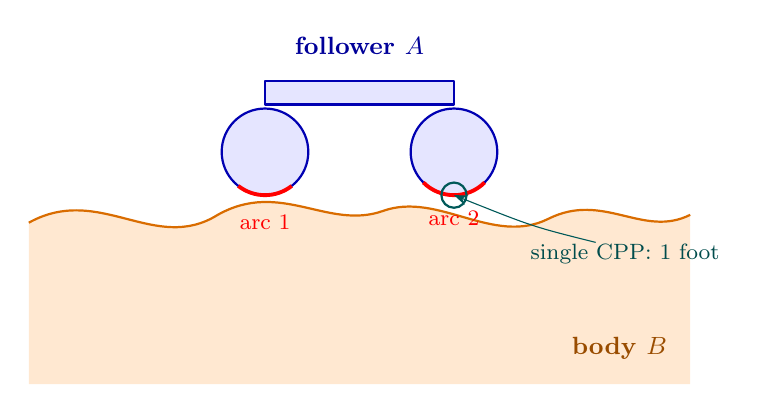
\begin{tikzpicture}[font=\footnotesize,>=Stealth,line join=round]
  % ---------- body B (gently wavy top, filled below) ----------
  \def\wavetop{
    (-4.2,0.45)
    .. controls (-3.3,0.95) and (-2.6,0.05) .. (-1.8,0.55)
    .. controls (-1.0,1.0)  and (-0.4,0.35) .. (0.3,0.6)
    .. controls (1.0,0.85)  and (1.7,0.15)  .. (2.4,0.5)
    .. controls (3.1,0.85)  and (3.6,0.25)  .. (4.2,0.55)
  }
  \fill[orange!18]
    \wavetop -- (4.2,-1.6) -- (-4.2,-1.6) -- cycle;
  \draw[orange!85!black,thick] \wavetop;
  \node[orange!60!black,font=\small\bfseries] at (3.3,-1.15) {body $B$};

  % ---------- follower A: two-footed staple ----------
  % circle centres
  \coordinate (cL) at (-1.2,1.35);
  \coordinate (cR) at ( 1.2,1.35);
  \def\rr{0.55}
  % top connecting bar
  \draw[blue!70!black,thick,fill=blue!10]
    (-1.2,1.95) -- (1.2,1.95) -- (1.2,2.25) -- (-1.2,2.25) -- cycle;
  % the two circular feet
  \fill[blue!10] (cL) circle (\rr);
  \fill[blue!10] (cR) circle (\rr);
  \draw[blue!70!black,thick] (cL) circle (\rr);
  \draw[blue!70!black,thick] (cR) circle (\rr);
  \node[blue!60!black,font=\small\bfseries] at (0,2.7) {follower $A$};

  % ---------- contact arcs dipping below the curve ----------
  % left foot: lower arc below curve (shallower contact)
  \draw[red,line width=1.4pt] ([shift=(232:\rr)]cL) arc (232:308:\rr);
  \node[red] at (-1.2,0.45) {arc 1};
  % right foot: lower arc below curve (deeper contact)
  \draw[red,line width=1.4pt] ([shift=(225:\rr)]cR) arc (225:315:\rr);
  \node[red] at (1.2,0.5) {arc 2};

  % ---------- single CPP on the deeper (right) contact ----------
  \coordinate (lp) at (1.2,0.8);              % lowest point of right foot
  \draw[teal!70!black,thick] (lp) circle (0.16);
  \node[teal!60!black,anchor=west] at (2.05,0.05)
    {single CPP: 1 foot};
  \draw[teal!70!black,->] (3.0,0.2) .. controls (2.2,0.4) .. (lp);
\end{tikzpicture}%
}
\caption{A boundary scan over body $A$'s chart evaluates the inverse-chart gap~\eqref{eq:radial-gap} at
every $\theta_A$ and marks the parameters with $\gn^B<0$. On a nonconvex pair these form two disjoint
contact arcs; a single closest-point projection returns only the globally nearest foot, missing the
second contact.}
\label{fig:tm-multiarc}
\end{figure}

\subsection{Inverting the chart in practice}\label{sec:tmap:invert}

% code: common/geometry.py::invert_decoder ; solvers/contact/profile_chart_2d.py::vertical_gap
The step that costs the most is inverting $B$'s chart, $\map{B}^{-1}$, and its cost depends on the chart
family. It takes three forms, in increasing order of work.

For \emph{radial charts} the inverse is closed form. The boundary parameter is just the direction angle
$\psi=\angle\,Q_B^\top(\xbf-c_B)$, computed by \code{atan2} in two dimensions or by normalizing
$Q_B^\top(\xbf-c_B)$ in three dimensions; the cost is $O(1)$ per query with no iteration.

For \emph{height charts} there is nothing to invert at all. The boundary is the graph $\map{}(x)=(x,h(x))$,
so the domain coordinate $x$ already \emph{is} the inverse-chart coordinate, and the transition map reads
off the gap by a single height comparison. The gap is how far the query point sits above the surface, and
the normal is perpendicular to the surface slope.
%
\begin{equation}\label{eq:height-gap}
g_{\mathrm{vert}}(x,z)=z-h_\theta(x),\qquad
\nbf=\frac{(-h_\theta'(x),\,1)}{\sqrt{1+h_\theta'^2(x)}}.
\end{equation}
%
Here $z$ is the height of the query point, $h_\theta(x)$ is the learned surface height at $x$, and
$h_\theta'(x)$ is its slope; the normal tilts away from vertical in proportion to that slope, and the
denominator normalizes it. The three-dimensional analogue is
$\nbf=(-h_x,-h_y,1)/\sqrt{1+\norm{\grad h}^2}$, built from the two surface slopes $h_x,h_y$. This is the
form the rough rock-joint detector of Section~\ref{sec:cv7} uses, and it is the reason that detector costs
$O(1)$ per query with no Newton solve.

For a general \emph{decoder chart} $D_B(\bm\xi)$ no closed form exists, so the inverse is found by Newton
iteration: we look for the parameter $\bm\xi$ whose image $D_B(\bm\xi)$ equals the query point $\xbf$, by
driving the residual $D_B(\bm\xi)-\xbf$ to zero.
%
\begin{equation}\label{eq:newton-invert}
\bm\xi^{(k+1)}=\bm\xi^{(k)}-J^{-1}\big(D_B(\bm\xi^{(k)})-\xbf\big),\qquad
J=\frac{\partial D_B}{\partial\bm\xi}.
\end{equation}
%
Here $\bm\xi^{(k)}$ is the $k$th guess, $J$ is the decoder Jacobian assembled by automatic
differentiation, and each step corrects the guess by the linearized residual. We stabilize the solve by
flooring the Jacobian's singular values and keeping the determinant consistent with the clamped spectrum,
which guards against a near-folded chart. The initial guess is the linear local-coordinate projection, and
the iteration runs until $\norm{D_B(\bm\xi)-\xbf}<10^{-8}$.

\subsection{A conservative-large but sign-exact gap}\label{sec:tmap:bias}

% code: solvers/contact/contact_manager.py::body_gap_normal
The radial inverse-chart gap buys its cheapness at one cost: it is not a true Euclidean distance. Because
it measures along the ray from the center rather than perpendicular to the surface, it overshoots the
perpendicular distance whenever the surface is tilted relative to the ray. The angle $\alpha$ is the tilt
between the ray direction $\dhat$ and the true surface normal at the radial foot, and $g_\perp$ is the
perpendicular (shortest) distance.
%
\begin{equation}\label{eq:radial-bias}
g_{\mathrm{rad}}=\frac{g_\perp}{\cos\alpha}+O(g^2)
\quad\Longrightarrow\quad
\abs{g_{\mathrm{rad}}}\ge\abs{g_\perp}\ \text{always}.
\end{equation}
%
Because $\cos\alpha\le1$, the radial gap $g_{\mathrm{rad}}$ is never smaller in magnitude than the
perpendicular gap $g_\perp$; the two agree only when the ray meets the surface head-on.
Figure~\ref{fig:tm-radial-bias} shows the geometry. The consequences are precise and benign. The sign of
$g_{\mathrm{rad}}$ is exact, so for star-shaped bodies the active set $\{\gn<0\}$ of penetrating points is
identical to the true level set's. The magnitude is conservative-large, so an exterior point reads a
slightly larger gap and a penetrating point a slightly deeper penetration; the penalty it produces is
marginally stiffer, never softer. The value equals the signed distance only on the sphere and in the
$g\to0$ limit.

The radial field is $C^1$ but not eikonal, meaning its gradient is continuous but not of unit length. In
deep concave valleys $\norm{\grad g}$ can reach $\sim10^4$, because the radial normal rotates rapidly there.
A perpendicular-foot refinement recovers the true normal-projected distance, but we use it only for
verification, because that foot jumps across the medial axis and would leak energy inside the integrator.

Swapping the chart detector in for the level set is a one-flag change. Declaring a body with the chart
detector routes its gap-normal dispatch to the radial evaluator instead of the signed-distance evaluator,
while the force laws, the broad-phase culler, and the MPM and FEM scatter all stay the same. Floors and
half-spaces, which are not star-shaped about any finite center, stay on the signed-distance path. The
transition map is therefore an opt-in detector that composes with the rest of the contact stack rather than
forking it. For height charts the matching statement is that~\eqref{eq:height-gap} is the small-slope-exact
normal-projected gap, not the closest-point distance; for those charts the fidelity story is the asperity
slopes, not the gap magnitude, as Section~\ref{sec:cv7} measures.

\begin{figure}
\centering
\resizebox{0.62\linewidth}{!}{%
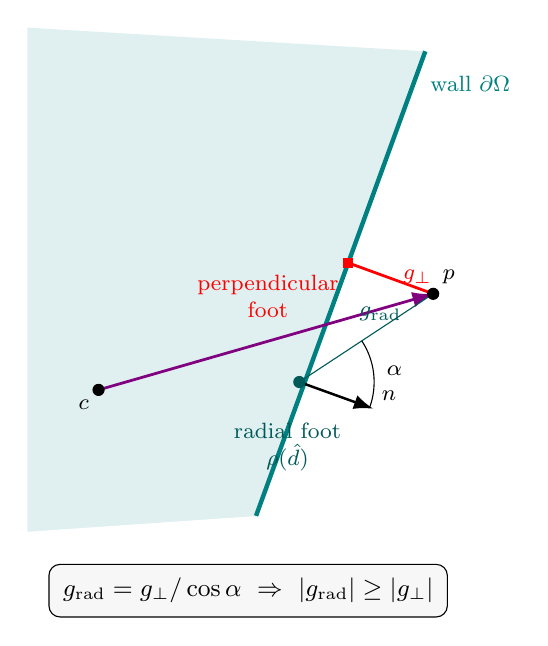
\begin{tikzpicture}[font=\footnotesize,>=Latex,line join=round]
  % ---- geometry ----------------------------------------------------------
  % wall inclined ~20 deg from vertical: direction (sin20, cos20)
  \coordinate (W1) at (1.30,-2.20);   % wall bottom
  \coordinate (W2) at (3.45, 3.70);   % wall top
  % interior point c (lower-left)
  \coordinate (c)  at (-0.70,-0.60);
  % radial foot on the wall (ray crossing)
  \coordinate (F)  at (1.85,-0.50);
  % exterior point p along the ray c->F, beyond the wall
  \coordinate (p)  at (3.55, 0.62);

  % ---- shaded interior side of the wall ----------------------------------
  \begin{scope}
    \clip (-1.6,-2.4) rectangle (4.6,4.0);
    \fill[teal!12]
      ($(W1)!1!(W2)$) -- (W1) -- (-1.6,-2.4) -- (-1.6,4.0) --
      ($ (W2) + (-1.6,0) $) -- (W2) -- cycle;
  \end{scope}
  % cleaner: just fill the half-plane left of the wall
  \begin{scope}
    \clip (-1.6,-2.4) rectangle (4.6,4.0);
    \fill[teal!12] (W1) -- (W2) -- (-1.6,4.0) -- (-1.6,-2.4) -- cycle;
  \end{scope}

  % ---- the wall (body boundary) ------------------------------------------
  \draw[teal,line width=1.6pt] (W1) -- (W2)
        node[pos=0.93,right=2pt,teal] {wall $\partial\Omega$};

  % ---- outward unit normal n at the radial foot --------------------------
  % outward = to the right of the wall; normal dir (cos20, -sin20) rotated:
  \coordinate (N) at ($(F)+(0.94,-0.34)$);
  \draw[->,black,line width=0.9pt] (F) -- (N) node[above right=-1pt,black] {$n$};

  % ---- radial ray  c -> foot -> p ----------------------------------------
  \draw[violet,line width=1.0pt,->] (c) -- (p);
  % along-ray gap segment foot->p (drawn in green over the ray)
  \draw[teal!70!black] (F) -- (p);

  % ---- perpendicular drop from p to the wall -----------------------------
  % foot of perpendicular from p onto line (W1)-(W2)
  \coordinate (Q) at ($(W1)!(p)!(W2)$);
  \draw[red,line width=1.0pt] (p) -- (Q);
  \draw[red,fill=red] ($(Q)+(-0.06,-0.06)$) rectangle ($(Q)+(0.06,0.06)$);
  \node[red,below left=1pt and 0pt of Q,align=center] {perpendicular\\ foot};

  % ---- angle alpha between normal and ray --------------------------------
  \pic[draw=black,angle radius=0.95cm,angle eccentricity=1.28,
       "$\alpha$"black] {angle = N--F--p};

  % ---- points ------------------------------------------------------------
  \fill[black] (c) circle (2.2pt) node[below left=0pt,black] {$c$};
  \fill[black] (p) circle (2.2pt) node[above right=0pt,black] {$p$};
  \fill[teal!70!black] (F) circle (2.2pt);
  \node[teal!70!black,below=10pt,align=center] at ($(F)+(-0.15,-0.05)$)
       {radial foot\\ $\rho(\hat d)$};

  % ---- segment labels ----------------------------------------------------
  \node[teal!70!black] at ($(F)!0.5!(p)+(0.18,0.30)$) {$g_{\mathrm{rad}}$};
  \node[red] at ($(p)!0.5!(Q)+(0.34,0.02)$) {$g_\perp$};

  % ---- boxed identity ----------------------------------------------------
  \node[draw,rounded corners,inner sep=5pt,fill=gray!6,align=center,
        font=\small] at (1.2,-3.15)
       {$g_{\mathrm{rad}}=g_\perp/\cos\alpha
         \ \Rightarrow\ |g_{\mathrm{rad}}|\ge|g_\perp|$};
\end{tikzpicture}%
}
\caption{On an inclined flank the ray from the center meets the surface at angle $\alpha$ to the true
normal, so the radial foot and the perpendicular foot differ and
$g_{\mathrm{rad}}=g_\perp/\cos\alpha\ge g_\perp$. The sign is exact, which yields the active-set
equivalence with the level set; the magnitude is conservative-large.}
\label{fig:tm-radial-bias}
\end{figure}

\section{Fourier-feature coordinate charts}\label{sec:fourier}

The transition map of Section~\ref{sec:tmap} reads contact off the boundary charts $\map{A}$ and
$\map{B}$. Its accuracy is therefore the accuracy of those charts as representations of the geometry. A
chart that smooths the asperity slopes returns a smoothed gap and a smoothed normal, and no
constraint-enforcement scheme downstream can recover the lost detail. This section states how the charts
are built and trained, and isolates the one ingredient that lets a small network resolve the sharp, rough,
cusped boundaries that an ambient level set (and a plain coordinate network) smooth away: a fixed
Fourier-feature encoding of the input. The level set, a neural signed-distance function, appears here only
as the baseline that the encoding has to beat. We treat it as a fair baseline, not a strawman, because it is
itself a coordinate network and suffers the same pathology a plain chart does.

\subsection{Spectral bias of a coordinate network}\label{sec:spectral}

A coordinate network is a function $f_\theta:\R^d\!\to\!\R$ given by a stack of affine maps and $\tanh$
nonlinearities fed the raw coordinate. Two of the objects this paper compares are exactly of this form:
an ambient neural signed-distance function $\Phi_\theta(\xbf)$ of the spatial point $\xbf\in\R^3$, and a
boundary chart $h_\theta(x)$ of the surface parameter $x$. Both are trained by regression onto sampled
data, and both inherit the same defect.

% code: rahaman2019spectral
A coordinate network learns the low-frequency content of its target first and the high-frequency content
slowly or not at all. This is the spectral bias of \citet{rahaman2019spectral}: in the
neural-tangent-kernel description of wide-network training, the kernel of a coordinate network is
approximately translation invariant and Laplace-like, so its eigenvalues decay with frequency and the
error in each Fourier mode of the target decays at a rate set by the corresponding eigenvalue. We can
make this rate explicit. Write the target as $\hat z(k)$ in frequency $k$ and the network output after
training time $t$ as $\hat f_\theta(k,t)$; the residual in each mode then shrinks geometrically, at its
own frequency-dependent speed,
%
% code: rahaman2019spectral
\begin{equation}\label{eq:ntk-decay}
\hat f_\theta(k,t)-\hat z(k)\ \approx\ \big(\hat f_\theta(k,0)-\hat z(k)\big)\,e^{-\eta\,\lambda(k)\,t},
\qquad \lambda(k)\sim \norm{k}^{-(d+1)},
\end{equation}
%
where $\eta$ is the learning rate and $\lambda(k)$ is the kernel eigenvalue for frequency $k$. The moving
part is $\lambda(k)$: it sets how fast mode $k$ converges, and because it falls off as a power of
$\norm{k}$, the high-$\norm{k}$ modes converge at a vanishing rate. At any finite training budget the
recovered surface is therefore a low-pass-filtered version of the true one. On a rough surface the
consequence is geometric. The asperities, cusps, and fine relief are filtered out, and what survives
is a smoothed envelope.

This is the failure mode of the ambient level set, and it is intrinsic rather than incidental. A neural SDF
cannot represent a boundary sharper than the highest frequency its training has resolved through
\eqref{eq:ntk-decay}; on a rock joint it flattens the asperity flanks, and through the strength law
$\muapp=\tan(\phi_b+i)$ of \citet{patton1966multiple} a flattened asperity angle $i$ directly
under-predicts the friction. The point to make precise, and the basis for the controlled ablation below,
is that \emph{a boundary chart of the raw coordinate inherits the identical pathology}. Representing the
geometry as a function on the surface's own parameter, rather than as an ambient field, does not by itself
buy any high frequencies; it changes the domain of $f_\theta$, not its spectral bias. The chart
parametrization alone does not beat the level set. The Fourier features do.

\subsection{The Fourier-feature encoding and three banks}\label{sec:banks}

% code: tancik2020fourier
The remedy of \citet{tancik2020fourier} is to replace the raw coordinate with a fixed (non-trainable) bank
of sinusoids applied before the network. Let $\tilde x\in[-1,1]^d$ be the input normalized to the unit box,
%
\begin{equation}\label{eq:normalize}
\tilde x = \frac{2(x-x_{\mathrm{lo}})}{x_{\mathrm{hi}}-x_{\mathrm{lo}}}-1,
\end{equation}
%
and let $B\in\R^{K\times d}$ be a bank of $K$ frequency vectors. The encoding and the chart are
%
% code: tancik2020fourier
\begin{equation}\label{eq:gamma}
\gamma(x)=\big[\cos(2\pi B\tilde x),\ \sin(2\pi B\tilde x)\big]\in\R^{2K},
\qquad
h_\theta(x)=\mathtt{base}+\mathrm{MLP}_\theta\!\big(\gamma(x)\big).
\end{equation}
%
The bank $B$ is a registered buffer, fixed for the life of the chart; only the network weights $\theta$ and
the scalar offset $\mathtt{base}$ (which carries the mean height, so the network learns only the deviation)
are trained. Prepending $\gamma$ changes the induced kernel from the Laplace-like form of
\eqref{eq:ntk-decay} to a stationary, band-limited one whose bandwidth is set by $B$. To see the new
kernel concretely, take the one-dimensional geometric bank below: the kernel becomes a finite sum of
cosines, one per chosen frequency $f_k$, and it depends only on the separation $\tilde x-\tilde x'$,
%
% code: tancik2020fourier
\begin{equation}\label{eq:kernel}
\Theta(x,x')=\frac1K\sum_{k=1}^{K}\cos\!\big(2\pi f_k\,(\tilde x-\tilde x')\big),
\end{equation}
%
so the network's similarity measure is built from exactly the frequencies in the bank and no others. For
the isotropic Gaussian bank the kernel is instead the radial profile $J_0(2\pi\sigma\norm{\tilde{\bm u}-\tilde{\bm
v}})$, flat out to a cutoff $\sim 2\pi\sigma$. Every frequency below the cutoff is now learned in parallel,
at a comparable rate, instead of in slow frequency order. The network no longer has to discover the high
frequencies; they are handed to it, and it learns only their amplitudes and phases. Two properties make
this the right tool for geometry. First, the cutoff is transparent and tunable. Where the level set's
smoothing is an intrinsic property of its architecture, the Fourier cutoff is an explicit knob ($f_{\max}$,
$\sigma$, or the harmonic order $K$), set to just resolve the finest wavelength required. Second, the bank
is deterministic and frozen, so the encoding is a reproducible preprocessing of the input rather than a
learned, run-dependent representation.

% code: solvers/contact/profile_chart_2d.py::NeuralHeight1D ; solvers/contact/surface_chart_3d.py::NeuralHeight2D ; solvers/contact/radial_chart_2d.py::NeuralRho2D
This paper uses three charts, and they differ only in two respects: the domain each one lives on, and
which bank of frequencies it uses to tile frequency space. The training loop is identical across all
three. Each bank is matched to its geometry. The geometric bank gives equal coverage on a
\emph{log}-frequency axis, which suits a profile with asperities spread across many wavelengths; the
Gaussian bank gives isotropic two-dimensional coverage, which suits a height field over a patch; and the
harmonic bank is periodic by construction, so a chart wrapped around the circle closes up on itself.
Table~\ref{tab:banks} collects the three banks, the charts they encode, and their parameters.

\begin{table}
\centering
\caption{The three Fourier banks and the charts they encode. The geometric bank gives equal coverage of
\emph{log}-scale, the Gaussian bank gives isotropic two-dimensional coverage, and the harmonic bank is
periodic by construction so a chart on the circle closes up. The bank $B$ is fixed; only the network and a
scalar offset are trained.}
\label{tab:banks}
\begin{tabular}{@{}llll@{}}
\toprule
Bank & Definition & Chart (file::class) & Parameters \\
\midrule
Geometric (deterministic) & $B=\operatorname{geomspace}(0.5,f_{\max},K)$ &
\code{NeuralHeight1D} ($h(x)$, $x\in\R$) & $K{=}192$, $f_{\max}{=}1500$ \\
Gaussian random & $B_i\sim\mathcal N(0,\sigma^2 I)$ &
\code{NeuralHeight2D} ($h(x,y)$) & $K{=}256$, $\sigma{=}8$ \\
Harmonic (periodic) & $[\cos(k\psi),\sin(k\psi)]_{k=1}^{K}$ &
\code{NeuralRho2D} ($\rho(\psi)$, $\psi\in\Sph^1$) & $K{=}16$ \\
\bottomrule
\end{tabular}
\end{table}

% code: solvers/contact/profile_chart_2d.py::NeuralHeight1D
The \emph{geometric} bank, $B=\operatorname{geomspace}(0.5,f_{\max},K)$ with $K=192$ and $f_{\max}=1500$,
spaces its frequencies equally in $\log$-scale and so resolves a wide range of asperity wavelengths with a
modest feature count; it carries the one-dimensional height chart $h_\theta(x)$ used for the rock-joint
profile, where the measured surface requires on the order of $L/\Delta x\approx 3000$ resolvable
wavelengths.
% code: solvers/contact/surface_chart_3d.py::NeuralHeight2D
The \emph{Gaussian random} bank, $B_i\sim\mathcal N(0,\sigma^2 I)$ with $K=256$ and $\sigma=8$, gives the
isotropic two-dimensional coverage appropriate to a height field $h_\theta(x,y)$ over a patch; its induced
kernel $J_0(2\pi\sigma\norm{\cdot})$ is flat to $\sim 2\pi\sigma$, the same Gaussian-relief encoding used by
the boundary-fitted volumetric decoder of Section~\ref{sec:form}.
% code: solvers/contact/radial_chart_2d.py::NeuralRho2D
The \emph{harmonic} bank, $[\cos(k\psi),\sin(k\psi)]_{k=1}^{K}$ with $K=16$, is periodic by construction;
this is mandatory, not a convenience, for the radial chart $\rho_\theta(\psi)$ on the circle
$\Sph^1$, where the radius must close up at $\psi=0,2\pi$. The radial chart additionally wraps its output in
a softplus, $\rho=\mathrm{softplus}(\mathtt{base}+\Delta)$, to keep $\rho>0$. Figure~\ref{fig:arch} shows
the encoding and the network it feeds.

\begin{figure}
\centering
\resizebox{\linewidth}{!}{%
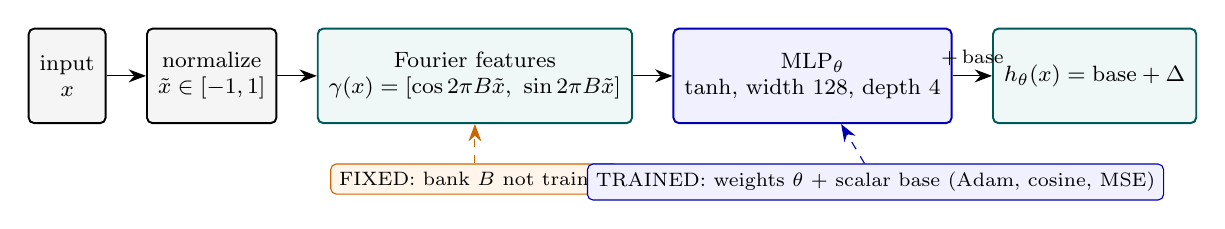
\begin{tikzpicture}[font=\footnotesize,>={Stealth[length=2.2mm]},
  box/.style={draw,rounded corners=2pt,align=center,inner sep=4pt,minimum height=12mm,line width=0.7pt},
  tag/.style={draw,rounded corners=2pt,align=center,inner sep=3pt,font=\scriptsize}]
  \node[box,fill=gray!8] (in) {input\\ $x$};
  \node[box,fill=gray!8,right=5mm of in] (nm) {normalize\\ $\tilde x\in[-1,1]$};
  \node[box,draw=teal!70!black,fill=teal!6,right=5mm of nm] (ff)
    {Fourier features\\ $\gamma(x)=[\cos 2\pi B\tilde x,\ \sin 2\pi B\tilde x]$};
  \node[box,draw=blue!70!black,fill=blue!6,right=5mm of ff] (mlp)
    {$\mathrm{MLP}_\theta$\\ tanh, width 128, depth 4};
  \node[box,draw=teal!70!black,fill=teal!6,right=5mm of mlp] (out)
    {$h_\theta(x)=\mathrm{base}+\Delta$};
  \draw[->] (in) -- (nm);
  \draw[->] (nm) -- (ff);
  \draw[->] (ff) -- (mlp);
  \draw[->] (mlp) -- (out) node[midway,above,font=\scriptsize]{$+\,\mathrm{base}$};
  \node[tag,draw=orange!80!black,fill=orange!8,below=5mm of ff] (t1) {FIXED: bank $B$ not trained};
  \node[tag,draw=blue!70!black,fill=blue!6,below=5mm of mlp,xshift=8mm] (t2)
    {TRAINED: weights $\theta$ + scalar base (Adam, cosine, MSE)};
  \draw[orange!80!black,->,dashed] (t1) -- (ff);
  \draw[blue!70!black,->,dashed] (t2) -- (mlp);
\end{tikzpicture}%
}
\caption{The Fourier-feature chart architecture, drawn for the one-dimensional height chart
\code{NeuralHeight1D}. The coordinate is normalized to $[-1,1]$ via \eqref{eq:normalize} and expanded by
the \emph{fixed} bank \eqref{eq:gamma} into $2K=384$ cosine/sine features; a plain $\tanh$ network (depth
$4$, width $128$) maps those to a scalar deviation $\Delta$, offset by the learnable mean $\mathtt{base}$.
Only the network weights $\theta$ and $\mathtt{base}$ are trained; the bank $B$ is frozen. The
two-dimensional and three-dimensional charts replace the geometric bank with a Gaussian one and the radial
chart wraps the output in a softplus, leaving the rest unchanged.}
\label{fig:arch}
\end{figure}

\subsection{Training and the verify-first protocol}\label{sec:train}

Every chart is trained by the same procedure: normalize the input by \eqref{eq:normalize}, encode with the
fixed bank \eqref{eq:gamma}, then regress the network onto sampled surface points by minibatch
mean-squared error,
%
\begin{equation}\label{eq:mse}
\mathcal L(\theta)=\frac{1}{\abs{\mathcal B}}\sum_{i\in\mathcal B}\big(h_\theta(x_i)-z_i\big)^2,
\end{equation}
%
with Adam at learning rate $2\times10^{-3}$ and a cosine annealing schedule that decays the rate to zero
over the iteration budget. The networks are small and are trained in double precision on CPU, which
conditions the geometry and the Jacobians used downstream; the random seed is fixed so a run is
reproducible. There is no adversary, no loss schedule, and no curriculum: a plain MSE regression suffices
because the Fourier encoding, not the optimizer, carries the high frequencies.

A trained chart \emph{is} geometry, and a corrupted chart silently corrupts every downstream solve, so a
chart is admitted to a contact computation only after three checks. (i) \emph{Reconstruction fidelity}: the
RMSE on the sampled surface points, reported as a fraction of the surface RMS, must reach a few percent.
(ii) \emph{No element foldover}: for the volumetric decoder the chart-Jacobian determinant must satisfy
$\det J>0$ on every element, since a folded chart has no valid pushforward. (iii) \emph{Discretization
convergence}: a manufactured-solution study on the curved chart geometry must recover the $O(h^2)$ rate of
the underlying P1 chart finite-element method, confirming that the trained geometry did not spoil the
solver. A chart that fails, with relief amplitude too high so $\det J$ folds, or cutoff too low so the
surface is under-resolved, is rejected, not patched.

% code: solvers/contact/profile_chart_2d.py::NeuralHeight1D
The clearest measurement of the Fourier contribution is the framework's own ablation, run on the real
Inada-granite tensile-fracture profile \citep{inada2020digitalrocks}, a self-affine surface with RMS
$\approx 1.7$~mm. The same network, with identical width, depth, optimizer, and schedule, is trained
twice on the measured points, once with the Fourier features active and once on the raw coordinate (the
\code{plain=True} control). Because a measured profile is a deterministic surface to represent, the metric
is reconstruction RMSE on the measured points, and the bank is band-limited below the sampling Nyquist so
the fit is well posed rather than an interpolation to zero. Figure~\ref{fig:curves} reports the two
training curves and the recovered surfaces. With the Fourier features the chart descends through the
asperity scales to a reconstruction RMSE of $0.003\%$ of the RMS and recovers this ablation window's mean
slope angle, here $\bar i = 19.9^\circ$ (the full-profile capstone below measures the surface's mean angle
as $19.4^\circ$). The byte-for-byte identical network on the raw coordinate plateaus at a spectral-bias
floor of $7.6\%$ of RMS ($136~\mu\mathrm{m}$) and
low-passes the slopes to $\bar i = 11.5^\circ$. The two networks differ only in the input encoding, and one
converges to the surface while the other stalls at a smoothed approximation. This is the chart-versus-level-set
thesis reduced to its mechanism, on a real surface.

\begin{figure}
\centering
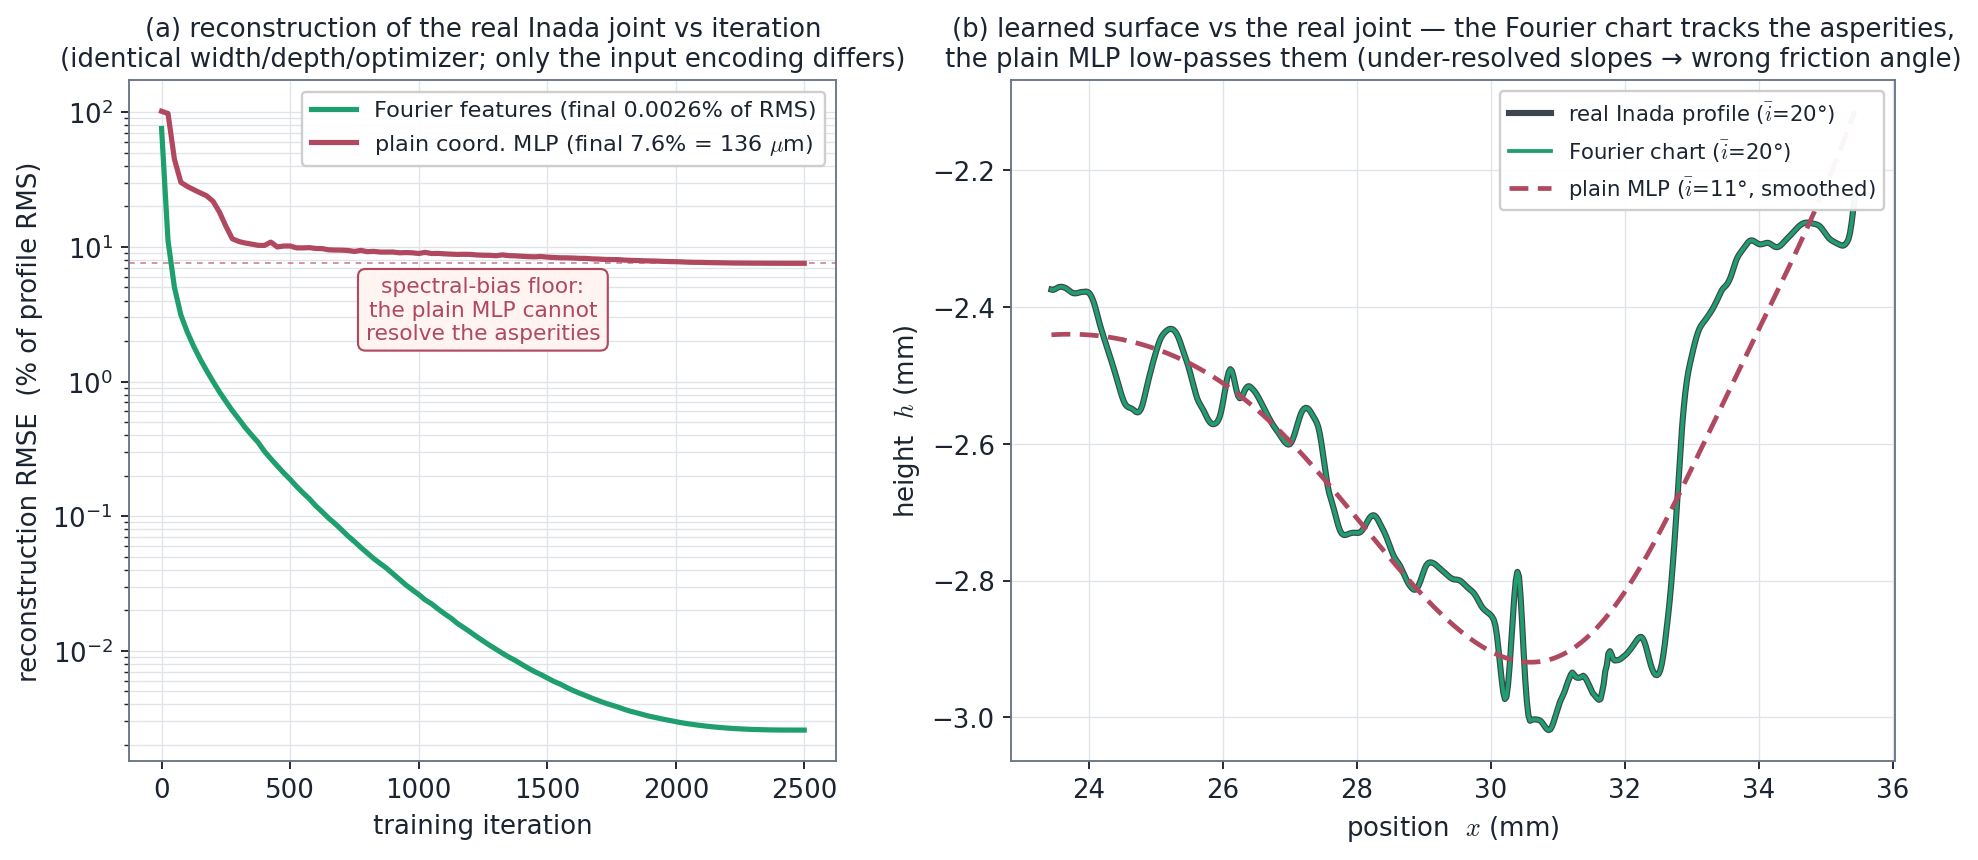
\includegraphics[width=\linewidth]{fourier_training_curves_pub}
\caption{Genuine training on the real Inada-granite profile \citep{inada2020digitalrocks}, both runs using
the repository's own \code{NeuralHeight1D}. (a) Reconstruction RMSE versus iteration: the Fourier chart
descends to $0.003\%$ of the surface RMS, while the \emph{identical} network fed the raw coordinate
plateaus at a $7.6\%$ ($136~\mu$m) spectral-bias floor; only the input encoding differs. (b) The learned
surfaces: the Fourier chart tracks the asperities and recovers the profile's mean slope angle $\bar i=19.9^\circ$,
whereas the plain network low-passes them to $\bar i=11.5^\circ$, under-resolving the slopes that set the
friction angle through $\muapp=\tan(\phi_b+i)$.}
\label{fig:curves}
\end{figure}

% code: solvers/fem/rough_block_decoder.py
The same separation holds for the boundary-fitted volumetric decoder used by the chart finite-element
method of Section~\ref{sec:form}, where the relief is carried by the Gaussian bank. The Fourier
decoder reconstructs the rough face to $2.2\%$ of RMS, a vanilla $\tanh$ decoder of equal capacity reaches
only $48\%$ (the spectral-bias floor again), and an ambient three-dimensional neural SDF of the same surface
reaches $15.7\%$; the decoder additionally passes $\det J>0$ on every element and the $O(h^2)$
manufactured-solution check (measured rates $2.07$ and $1.83$). On the one-dimensional Inada profile, the
production height chart ($K=192$, $f_{\max}=1500$) reconstructs the surface to $2.3~\mu\mathrm{m}$, about
$0.1\%$ of the $1.7$~mm RMS, while the ambient neural SDF of the same surface reaches only
$107~\mu\mathrm{m}$, which is $47\times$ worse with \emph{more} parameters, and smooths the mean asperity
angle from $19.4^\circ$ to $12.5^\circ$. Through the Patton law that smoothing under-predicts the peak shear
strength by $61\%$; the asperity slopes the chart preserves are precisely the geometry that drives the
contact mechanics.

\subsection{Why charts beat the level set}\label{sec:why}

The advantage is a property of the kernel, not of the parametrization. The level set is a coordinate
network of the ambient point and therefore carries the Laplace-like kernel of \eqref{eq:ntk-decay}, whose
spectral ceiling is an intrinsic, non-tunable consequence of the architecture; on rough or cusped geometry
it filters away exactly the high frequencies that contact cares about. The Fourier-feature chart carries
the stationary, band-limited kernel of \eqref{eq:kernel} instead, with a cutoff one sets explicitly to
resolve the finest wavelength of interest and no spectral ceiling below it. The chart also stores geometry
as a surface function, so its cost scales with the surface rather than with an ambient volume, but the
fidelity argument rests on the kernel.

The ablation of Section~\ref{sec:train} is the load-bearing evidence: the Fourier features, not the chart
parametrization alone, do the work. A chart of the raw coordinate (\code{plain=True}) smooths the Inada
profile to the same $7.6\%$ floor and the same $11.5^\circ$ angle that the level set produces, because it
inherits the same spectral bias; only when the fixed sinusoidal bank is prepended does the reconstruction
fall to $0.003\%$ and the slope angle become exact. We therefore do not claim that reading geometry off a
boundary chart is, by itself, more accurate than reading it off a level set. On a smooth surface dense
interpolation is easy for either, and the height RMSE of a well-resolved SDF is not the discriminating
quantity. The claim is sharper and is the one the measurements support: the level set smooths asperity
slopes through an intrinsic spectral ceiling and so under-predicts strength and dilatancy, whereas a
Fourier-feature chart has a transparent, tunable cutoff and resolves those slopes. The scope is that
the height and surface charts represent single-valued geometry (no overhangs) and that the harmonic radial
chart requires star-shaped boundaries; the band-limit is a chosen resolution, not an unlimited one. Within
that scope the encoding is what converts a smoothing approximator into a faithful one, and every downstream
result in this paper rests on it.

\section{Contact formulation and discretization}\label{sec:form}

The transition map of Section~\ref{sec:tmap} acts as a geometric oracle: queried at any point, it
reports two numbers that a contact solver needs and nothing more. The first is the gap $\gn$, the
signed distance from the point to the obstacle surface. The second is the outward unit normal $\nbf$,
the direction along which contact pushes. The atlas reads this pair from the boundary-to-boundary
chart map $\tmap=\map{B}^{-1}\circ\map{A}$, which composes the inverse of one body's boundary chart
with the other's. A neural signed-distance function (a level set) supplies the same pair as a
comparison baseline. This section places that oracle inside a standard contact solver and keeps the
two sources interchangeable.

Everything the solver does with $(\gn,\nbf)$ is classical, and we want the reader to see that nothing
in it depends on where the pair came from. The constraint enforcement (penalty and augmented
Lagrangian), the friction law, the consistent Newton tangent, and the spatial discretization are all
textbook constructions. We route them through a single interface that returns $(\gn,\nbf)$, so that
force assembly, broad phase, tangent, and well-posedness are byte-for-byte identical whether the
geometry comes from the atlas or from the level set. The accuracy gap reported in
Sections~\ref{sec:verif}--\ref{sec:cv7} is therefore charged to the geometry alone, not to the
constraint solver.

We fix the sign convention once. The gap $\gn(\xbf)$ is the signed distance from a candidate contact
point $\xbf$ to the obstacle surface: positive when the bodies are apart, negative when they overlap,
so $\gn<0$ flags penetration. The normal $\nbf$ points outward from the obstacle, which makes the
contact force $-t_N\nbf$ push a penetrating point back out, where $t_N\ge0$ is the contact pressure.
We write $\pos{\cdot}$ for the Macaulay bracket $\pos{a}=\max(0,a)$, which returns a quantity only
when it is positive, and zero otherwise.

\subsection{Signorini conditions and the contact potential}\label{sec:form-signorini}

% code: solvers/contact/augmented_lagrangian.py
Contact is governed by three plain physical rules: bodies may not interpenetrate, contact only
pushes and never pulls, and pressure builds up only where the surfaces actually touch. We state them
for two deformable bodies $\Omega^A,\Omega^B\subset\R^3$ that undergo displacement fields
$\ubf^A,\ubf^B$ and may meet along a candidate contact surface $\Gamma_c$ in the deformed
configuration. The three rules become the Signorini--Hertz--Moreau conditions, which are the
Karush--Kuhn--Tucker (KKT) optimality conditions of the constrained problem,
\begin{equation}\label{eq:signorini}
\gn\ \ge\ 0,\qquad t_N\ \ge\ 0,\qquad \gn\, t_N\ =\ 0\qquad\text{on }\Gamma_c .
\end{equation}
Reading them in order: the first inequality forbids penetration; the second forbids tensile
(adhesive) tractions, so the surface can push but not glue; and the complementarity $\gn t_N=0$ ties
the two together, allowing pressure only where the gap has closed to zero. These unilateral
conditions of \citet{johnson1985contact} and \citet{wriggers2006computational} are what make
equilibrium a variational inequality rather than a smooth minimization
\citep{kikuchi1988contact,laursen2002computational}: the active contact set is itself an unknown.

We now write equilibrium in weak (virtual-work) form so that the contact pressure enters as a force
on the boundary. Let
$a^\alpha(\ubf^\alpha,\delta\ubf^\alpha)=\int_{\Omega^\alpha}\bm{P}(\bm{F}^\alpha):\grad_{\xbf}\delta\ubf^\alpha\,dV$
be the internal virtual work of body $\alpha\in\{A,B\}$, in which $\bm{P}$ is the first
Piola--Kirchhoff stress, $\bm{F}^\alpha=\bm{I}+\grad\ubf^\alpha$ is the deformation gradient, and
$\delta\ubf^\alpha$ is an admissible virtual displacement; let $L^\alpha$ collect the external
virtual work of the body and surface loads. We need one more ingredient: how the gap responds to a
virtual displacement. Because the gap is a distance measured along the normal, its first variation is
just the relative virtual motion projected onto $\nbf$,
\begin{equation}\label{eq:gap-variation}
\delta\gn\ =\ \nbf\cdot(\delta\ubf^B-\delta\ubf^A),
\end{equation}
which uses only the contact normal and is exact to first order no matter how the surface is
represented. This is the key point for the atlas-versus-level-set comparison: the variation depends on
the geometry through $\nbf$ alone. Constrained equilibrium then reads: find $(\ubf^A,\ubf^B)$ and a
pressure multiplier $t_N\ge0$ such that
\begin{equation}\label{eq:weak-contact}
\sum_{\alpha\in\{A,B\}}\!\Big[a^\alpha(\ubf^\alpha,\delta\ubf^\alpha)-L^\alpha(\delta\ubf^\alpha)\Big]
\ +\ \int_{\Gamma_c} t_N\,\delta\gn\,dA\ =\ 0,
\end{equation}
holds together with the Signorini conditions~\eqref{eq:signorini}. The new term is the contact
integral: the pressure $t_N$ does virtual work against the gap variation along $\Gamma_c$. What
remains is to supply $t_N$, and the next two paragraphs give the two standard ways to do so.

\paragraph{Penalty regularization: a stiff one-sided spring.}
% code: solvers/contact/penalty.py::compute_contact_force
The penalty method replaces the exact pressure by a stiff spring that switches on only when the
constraint is violated. Picture a spring that does nothing while the bodies are apart and pushes back
ever harder the deeper they overlap. With penalty stiffness $\varepsilon_n>0$ the pressure is
\begin{equation}\label{eq:penalty-pressure}
t_N\ =\ \varepsilon_n\,\pos{-\gn},
\end{equation}
which is zero whenever $\gn\ge0$ and rises linearly with the penetration depth $-\gn$ once the bodies
overlap. The spring stores energy as it compresses, and that stored energy is the smooth contact
potential,
\begin{equation}\label{eq:penalty-potential}
\Pi_c(\gn)\ =\ \tfrac{1}{2}\varepsilon_n\,\pos{-\gn}^2,
\qquad
t_N\ =\ \frac{\partial \Pi_c}{\partial(-\gn)}\ =\ \varepsilon_n\,\pos{-\gn} .
\end{equation}
Differentiating the potential recovers the pressure~\eqref{eq:penalty-pressure}, which tells us the
normal contact force is conservative: it is the gradient of a scalar energy. Because that energy is
non-negative, adding it to the total potential keeps the problem coercive, the property used in
Section~\ref{sec:form-wellposed}. The force carried by one quadrature point (or, in the meshfree
setting, one particle) in physical space then follows from the pressure,
\begin{equation}\label{eq:penalty-force}
\fbf^{\,\mathrm{N}}\ =\ t_N\,A\,\nbf\ =\ \varepsilon_n\,\pos{-\gn}\,A\,\nbf ,
\end{equation}
where $A$ is the tributary area carried by that point (or the particle volume $V_p$ in the MPM
coupling of Section~\ref{sec:form-mpm}). The force points along the normal and scales with both the
penetration and the stiffness. Equation~\eqref{eq:penalty-force} is exactly what
\code{compute\_contact\_force} in \code{solvers/contact/penalty.py} does: clamp $-\gn$ to its positive
part, scale by $\varepsilon_n A$, and project onto the obstacle normal. We size the spring to the
material it restrains, $\varepsilon_n=\beta E/h$, with $\beta\in[1,20]$, $E$ the Young modulus, and
$h$ the local mesh size, so the contact stiffness matches the bulk stiffness. The leftover penetration
then scales as $\delta\sim\sigma_n/\varepsilon_n$ and shrinks as $\varepsilon_n$ grows.

\paragraph{Augmented Lagrangian: a spring whose rest force is remembered.}
% code: solvers/contact/augmented_lagrangian.py
The penalty spring forces a compromise: a stiffer $\varepsilon_n$ shrinks the residual penetration but
worsens the conditioning of the system, and in explicit dynamics it shortens the stable time step. The
augmented-Lagrangian method of \citet{alart1991mixed} and \citet{simo1992augmented} escapes the
compromise by giving the spring a memory. Alongside the penalty it carries a persistent multiplier
$\lambda\ge0$ that remembers the pressure accumulated so far, so the spring no longer has to supply the
full pressure from penetration alone. The augmented pressure and its Uzawa update are
\begin{equation}\label{eq:al-pressure}
t_N\ =\ p_{\mathrm{aug}}(\gn,\lambda)\ =\ \pos{\lambda-\varepsilon_n\,\gn},
\qquad
\lambda^{k+1}\ =\ \pos{\lambda^{k}-\varepsilon_n\,\gn(\ubf^{k+1})} .
\end{equation}
Reading the update: with $\gn<0$ on overlap, the term $-\varepsilon_n\gn$ is positive, so both the
pressure and the remembered multiplier grow while penetration persists; once the gap closes
($\gn\ge0$) the Macaulay clamp drives both back to zero. The payoff is that at convergence the memory
$\lambda$ settles on the true contact pressure, $\lambda\to t_N^\star$, and the penetration vanishes
without sending $\varepsilon_n\to\infty$ \citep{laursen2002computational}. This is
\code{AugmentedLagrangianContact} in \code{solvers/contact/augmented\_lagrangian.py}; the solver stores
$\lambda$ per contact point and reuses it across iterations, so the caller must pass the gap with
stable indexing (the implementation resets $\lambda$ and warns if the array shape changes between
calls). The plain penalty~\eqref{eq:penalty-pressure} is the special case with no memory,
$\lambda\equiv0$.

\subsection{Regularized Coulomb friction}\label{sec:form-friction}

% code: solvers/contact/friction.py
Once contact carries a normal pressure, friction resists tangential sliding. The Coulomb law caps the
tangential traction $\tbf_T$ by the friction cone $\norm{\tbf_T}\le\mu\,t_N$: inside the cone the
surfaces stick ($\vbf_T=0$), and on its boundary they slip with
$\tbf_T=-\mu t_N\,\vbf_T/\norm{\vbf_T}$, where $\mu$ is the friction coefficient and $\vbf_T$ the
tangential slip velocity \citep{wriggers2006computational}. This law has a kink at zero sliding speed
that a Newton solver cannot differentiate, so we smooth it. We replace the sharp law by the
bracket form
\begin{equation}\label{eq:friction-reg}
\tbf_T\ =\ -\,\mu\,\norm{\fbf^{\,\mathrm{N}}}\,
\frac{\vbf_T}{\sqrt{\norm{\vbf_T}^2+\varepsilon_T^2}},
\end{equation}
in which the tangential velocity is the full velocity with its normal component removed,
\begin{equation}\label{eq:vt-projection}
\vbf_T\ =\ \big(\bm{I}-\nbf\otimes\nbf\big)\,\vbf\ =\ \vbf-(\vbf\cdot\nbf)\,\nbf .
\end{equation}
The parameter $\varepsilon_T$ is a small velocity scale that controls the rounding of the kink. When
sliding is fast, $\norm{\vbf_T}\gg\varepsilon_T$, the traction approaches the cone bound
$\mu\norm{\fbf^{\,\mathrm{N}}}$ and the law behaves like sharp Coulomb slip; when sliding is slow,
$\norm{\vbf_T}\ll\varepsilon_T$, the traction grows linearly with $\vbf_T$ and passes smoothly through
zero, so stick is approximated by a stiff tangential spring. Like the penalty, this surrogate comes
from a potential: the pseudo-potential
$\Psi_T(\vbf_T)=\mu\,t_N\sqrt{\norm{\vbf_T}^2+\varepsilon_T^2}$ yields
$\tbf_T=-\partial\Psi_T/\partial\vbf_T$, so the regularized problem stays variational. In code,
\code{compute\_friction\_force} in \code{solvers/contact/friction.py} takes the scalar normal-force
magnitude $\norm{\fbf^{\,\mathrm{N}}}$ as input, so it composes unchanged with either normal model: the
penalty pressure ($\norm{\fbf^{\,\mathrm{N}}}=\varepsilon_n\pos{-\gn}A$) or the augmented-Lagrangian
pressure ($\norm{\fbf^{\,\mathrm{N}}}=p_{\mathrm{aug}}A$). The total contact force is then the sum of
normal and tangential parts, $\fbf^{\,\mathrm{contact}}=\fbf^{\,\mathrm{N}}+\tbf_T A$. By construction
the friction force opposes the slip, $\tbf_T\cdot\vbf_T\le0$, which the verification suite confirms
node by node.

The quasi-static rough-joint driver of Section~\ref{sec:cv7} has no sliding velocity to regularize, so
there we drive friction differently. We drag each active node along a prescribed full-slip direction
$\tbf_{\mathrm{proj}}=\widehat{\hat{\tbf}-(\hat{\tbf}\cdot\nbf)\nbf}$, formed by projecting the loading
direction $\hat{\tbf}$ onto the tangent plane and renormalizing, and set
$\tbf_T=\mu\,t_N\,\tbf_{\mathrm{proj}}$. The velocity surrogate~\eqref{eq:friction-reg} is instead the
path used in the explicit MPM cross-check. Both sit at the cone bound and are plain Coulomb, and
neither imposes a dilation angle. The dilatant, slope-dependent response seen in
Section~\ref{sec:cv7} is therefore not put in by hand. It emerges from the resolved asperity geometry
through the normal $\nbf$, rather than from a constitutive dilation law of the
Patton~\citep{patton1966multiple} or Barton~\citep{barton1977shear,barton1990review} type.

\subsection{Consistent contact tangent}\label{sec:form-tangent}

% code: benchmarks/contact/cv_numerical/rock_joint_decoder_shear.py::_contact_tangent
A Newton solver needs the derivative of the contact force with respect to the displacement; supplying
the right derivative is what makes Newton converge quadratically. Writing the residual as
$\bm{R}(\ubf)=\bm{K}_{\mathrm{elastic}}\ubf-\fbf_{\mathrm{contact}}(\ubf)$, the contact part of the
tangent at an active node ($\gn<0$) gathers three contributions,
\begin{equation}\label{eq:contact-tangent}
\bm{K}_c\ =\ \frac{\partial \fbf_{\mathrm{contact}}}{\partial \ubf}
\ =\ \underbrace{\varepsilon_n A\,\big(\nbf\otimes\nbf\big)}_{\text{normal penalty stiffness}}
\ +\ \underbrace{\varepsilon_n A\,\mu\,\big(\tbf_{\mathrm{proj}}\otimes\nbf\big)}_{\text{friction--normal coupling}}
\ +\ \underbrace{t_N A\,\frac{\partial\nbf}{\partial\ubf}}_{\text{curvature / shape operator}} .
\end{equation}
Each term answers a distinct question. The first is the normal stiffness: it is the penalty stiffness
$\varepsilon_n A$ projected onto the active normal through $\nbf\otimes\nbf$, and it tells Newton how
the normal force stiffens as the node sinks in. Because $\nbf$ tilts with the asperity slope,
$\nbf\otimes\nbf$ is a full rank-one $3\times3$ block, not the single vertical stiffness a
flat-interface model would assume, so a tilted asperity already couples the vertical and horizontal
directions. The second term is the friction--normal coupling: it tells Newton how the frictional drag
changes when the normal pressure changes. It is non-symmetric, which is the structural signature of a
non-associative friction law \citep{wriggers2006computational}. The third term is the curvature (or
geometric) stiffness: it accounts for the normal direction itself rotating as the surface deforms,
which matters wherever the surface bends. That rotation is the shape operator (the Weingarten map) of
the contact surface,
\begin{equation}\label{eq:shape-operator}
\frac{\partial n_i}{\partial x_j}
\ =\ \frac{1}{\norm{\grad\phi}}\,\big(\delta_{ik}-n_i n_k\big)\,
\frac{\partial^2\phi}{\partial x_k\partial x_j},
\end{equation}
which the surface description supplies through its second derivative: either second-order autograd on
the neural SDF, or the second derivative $h_\theta''$ of the Fourier-feature height chart. In
practice, the rough-joint driver assembles the first two terms (this is
\code{\_contact\_tangent}). On the smooth single-asperity benchmarks the curvature term is small, so
keeping only the rank-one normal and friction--normal blocks, with an Armijo line search, still drives
the frictional Newton residual down to $\sim10^{-9}$ on the one-block shear, a fully converged solve.
One configuration resists this convergence. On the two-deformable, moving-master node-to-surface
problem the friction residual settles at $1.5$--$6\%$ and does not shrink under mesh refinement,
because the contact point itself moves and makes the active set non-smooth. The remedy there is a
semismooth-Newton, augmented, or mortar treatment
\citep{alart1991mixed,puso2004mortar,chouly2013nitsche}, not a finer mesh.

\subsection{Discretization: chart-FEM pushforward and physical-space MPM}\label{sec:form-mpm}

We enforce the contact constraint on two discretizations: a chart-based finite element method and a
chart-based material point method. Both share the same force expressions and the same $(\gn,\nbf)$
oracle. They differ only in how they carry the geometry of the chart, and the contrast between the two
is the point of this subsection.

\paragraph{Chart-FEM pushforward.}
% code: solvers/fem/chart_vector_fem.py
The chart-FEM solves the elasticity problem on a simple reference cube and then maps it onto the curved
physical body. Concretely, on each chart the elastostatic problem lives on the reference parametric
cube $U_i=[-r,r]^3$, and the chart decoder $\map{i}$ carries it to physical space through its Jacobian
$\bm{J}_i=\partial\map{i}/\partial\bm{\xi}$, the matrix of derivatives of the physical coordinate with
respect to the reference coordinate $\bm{\xi}$. Gradients computed on the cube must be converted to
physical gradients by the chain rule, which means multiplying by $\bm{J}_i^{-1}$,
\begin{equation}\label{eq:fem-pushforward}
\grad_{\xbf}\ubf\ =\ \grad_{\bm{\xi}}\ubf\,\bm{J}_i^{-1},
\qquad
\bm{F}\ =\ \bm{I}+\grad_{\bm{\xi}}\ubf\,\bm{J}_i^{-1},
\end{equation}
so $\grad_{\xbf}\ubf$ is the physical displacement gradient and $\bm{F}$ the physical deformation
gradient. The same chain rule and the change-of-variables volume factor $\abs{\det\bm{J}_i}$ then turn
the cube integral into the physical stiffness,
\begin{equation}\label{eq:fem-assembly}
\bm{K}_{ab}\ =\ \int_{U_i}\big(\grad_{\bm{\xi}}N_a\,\bm{J}_i^{-1}\big)^{\!\top}
:\mathbb{C}:\big(\grad_{\bm{\xi}}N_b\,\bm{J}_i^{-1}\big)\,\abs{\det\bm{J}_i}\,d\bm{\xi},
\end{equation}
where $N_a,N_b$ are the shape functions and $\mathbb{C}$ is the elasticity tensor. The one subtlety is
that a neural chart can be steep, which makes $\bm{J}_i$ nearly singular and $\bm{J}_i^{-1}$ large. We
therefore form $\bm{J}_i^{-1}$ and $\abs{\det\bm{J}_i}$ through the SVD-clamped operator
\code{stabilized\_jacobian\_ops} (\code{solvers/fem/chart\_vector\_fem.py}), which floors the singular
values so a poorly conditioned chart cannot blow up the assembly, while $\det\bm{J}_i>0$ (no fold-over)
is monitored throughout. On the boundary-fitted rough geometry this pushforward passes a patch test and
recovers the manufactured-solution rate $O(h^2)$ (measured exponents $2.07$ and $1.83$), which
confirms that the discretization error is controlled independently of the contact treatment. The
penalty force $\fbf^{\,\mathrm{N}}=\varepsilon_n\pos{-\gn}A\,\nbf$ enters the chart residual
work-conjugately, with $A$ the tributary boundary-face area measured in physical space.

\paragraph{MPM coupling in physical space.}
% code: docs/contact_theory_manual.md section 1.2
The material point method needs no such pushforward for the contact force, and this is the point to
isolate. The chart-based MPM stores particle velocity, gravity, and stress directly in physical
space, so the contact force is added through the same particle-to-grid (P2G) channel as gravity,
with \emph{no Jacobian pull-back},
\begin{equation}\label{eq:mpm-p2g}
\fbf_I^{\mathrm{ext}}\ \mathrel{+}=\ \sum_p \fbf_p^{\,\mathrm{contact}}\,N_I(\bm{\xi}_p),
\qquad
\fbf_p^{\,\mathrm{contact}}\ =\ \varepsilon_n\,\pos{-\gn(\xbf_p)}\,V_p\,\nbf_p\ +\ \tbf_T\,V_p ,
\end{equation}
where $N_I$ is the grid shape function and $\xbf_p=\map{i}(\bm{\xi}_p)+\ubf_p$ is the particle's
physical position. The volume factor $V_p$ converts the penalty pressure into a force (pressure times a
volume), so $\fbf_p^{\,\mathrm{contact}}$ scatters to the grid like any other force: without the mass
weight that gravity carries, and without the $\bm{J}_i^{-\top}$ that a chart-local force would need.
Put plainly, forces and grid velocities already live in the same physical space, so the contact force
is added verbatim, and that is the central bookkeeping point of the MPM coupling. The penalty spring
also adds its own stability bound to the explicit time step,
$\Delta t_{\mathrm{contact}}\le 0.5\sqrt{m_{\min}/\varepsilon_n}$, so the effective step is the smaller
of the elastic CFL limit and this contact limit, $\min(\Delta t_{\mathrm{CFL}},\Delta
t_{\mathrm{contact}})$. The MPM path reproduces the Coulomb floor, returning an apparent friction
$\muapp\approx0.34$ against an imposed $\mu=0.4$, but it does not reproduce the dilatancy, because a
mated rough-on-rough block is unstable in explicit penalty dynamics. We therefore use the MPM as a
dynamic cross-check rather than as the primary rough-joint solver, and we mark that limit plainly.

\subsection{Level-set-free detector dispatch}\label{sec:form-dispatch}

% code: solvers/contact/contact_manager.py::body_gap_normal
The geometry enters the solver at exactly one place, by design. A single function
\code{body\_gap\_normal} takes a batch of physical-space query points and returns the pair
$(\gn,\nbf)$, choosing its source according to the body's declared detector,
\begin{equation}\label{eq:detector-dispatch}
(\gn,\nbf)\ =\
\begin{cases}
\big(\phi_A(\xbf),\ \grad\phi_A/\norm{\grad\phi_A}\big), & \text{detector} = \texttt{sdf},\\[4pt]
\texttt{evaluate\_gap\_chart}(\xbf,\ \text{chart}), & \text{detector} = \texttt{chart}.
\end{cases}
\end{equation}
Both branches honor the identical contract: $\gn$ has shape $(N,)$ with $\gn<0$ meaning penetration,
and $\nbf$ has shape $(N,3)$ and is a unit outward normal. The \texttt{sdf} branch evaluates the
neural level set $\phi_A$ and its autograd gradient; the \texttt{chart} branch evaluates the
transition-map detector of Section~\ref{sec:tmap}, which is the radial chart for star-shaped bodies, or
the height chart $\gn=z-h_\theta(x)$ with normal $(-h_\theta',1)/\sqrt{1+h_\theta'^2}$ for
single-valued joints. Everything downstream reads only $(\gn,\nbf)$: the broad-phase seed-to-seed cull,
the narrow-phase active-set selection $\{\gn<0\}$, the penalty and augmented-Lagrangian forces, the
friction law, the consistent tangent~\eqref{eq:contact-tangent}, and both discretizations. None of it
can tell which branch produced the pair. Swapping the atlas for the level set therefore touches one
branch of~\eqref{eq:detector-dispatch} and nothing else, and that is what makes the comparison
controlled: the same solver, the same loading, the same tolerances, with only the geometric oracle
changed.

% code: solvers/contact/contact_manager.py::body_gap_normal
Figure~\ref{fig:tm-levelset-vs-chart} puts the two oracles side by side on a rough profile. The atlas
detector resolves the asperity slopes; the level set, built from an ambient field whose spectral bias
favors low frequencies \citep{rahaman2019spectral}, smooths them away. The numbers follow the
picture. On the real Inada-granite joint, the chart detector returns a contact gap with $4.2\%$ RMS
error against the analytic surface, while the ambient SDF returns $44.7\%$. That is a factor of $10.5$
on the quantity that drives contact, and the chart reaches it at only $1.47\times$ the per-query cost
of the SDF and with no ambient field to store. That accuracy difference propagates. As
Section~\ref{sec:cv7} quantifies, the level set under-predicts the emergent dilatancy by $98\%$ and the
frictional strength by $35\%$, purely because it feeds the same solver a smoothed normal.

\subsection{Well-posedness and the penalty estimate}\label{sec:form-wellposed}

% code: contact_atlas/03_mathematical_theory.md
We close with the standard existence and stability statements. They carry over unchanged here, because
the contact treatment is classical and the chart changes only how the gap is evaluated, not the
analysis around it. Assume that each body's stored-energy density $W(\bm{F})$ is polyconvex with the
usual coercivity and growth bounds (the Neo-Hookean and small-strain models used here qualify), that
the admissible set $K=\{(\ubf^A,\ubf^B): \gn\ge0\text{ on }\Gamma_c\}$ is non-empty, that the body
loads lie in
$L^2(\Omega)$, and that the Dirichlet data lie in $H^{1/2}(\Gamma_D)$. The natural object to minimize is the
total energy, the stored elastic energy minus the work of the loads,
\begin{equation}\label{eq:total-energy}
E(\ubf^A,\ubf^B)\ =\ \sum_{\alpha\in\{A,B\}}\int_{\Omega^\alpha}W(\bm{I}+\grad\ubf^\alpha)\,dV
\ -\ \sum_{\alpha\in\{A,B\}}L^\alpha(\ubf^\alpha),
\end{equation}
and under these assumptions $E$ attains a minimizer on the admissible set $K$. The argument is the
direct method: polyconvexity gives weak lower semicontinuity of $E$, the growth bound keeps a
minimizing sequence bounded in $H^1\times H^1$, the trace inequality and the continuity of the gap
operator make $K$ weakly closed, and weak compactness then delivers the minimizer
\citep{ball1977convexity,ciarlet1988mathematical}. Adding the penalty changes nothing essential: the
penalty energy $\Pi_c$ of~\eqref{eq:penalty-potential} is non-negative and convex in $\gn$, so adding
it to $E$ preserves both lower semicontinuity and coercivity, and the penalized problem is well posed
for every $\varepsilon_n>0$.

% code: contact_atlas/03_mathematical_theory.md
The remaining question is how close the penalty solution lands to the exact one, and how that closeness
depends on the stiffness. Let $\ubf_\varepsilon$ be the penalty solution and $\ubf^\star$ the exact
(multiplier) solution. The standard estimate of \citet{kikuchi1988contact} bounds their difference in
terms of the penalty stiffness,
\begin{equation}\label{eq:penalty-estimate}
\norm{\ubf_{\varepsilon}-\ubf^\star}_{H^1}\ \le\ \frac{C}{\sqrt{\varepsilon_n}},
\qquad
\norm{t_{N,\varepsilon}-t_N^\star}_{H^{-1/2}(\Gamma_c)}\ \le\ C\sqrt{\varepsilon_n},
\end{equation}
so the displacement converges at rate $O(\varepsilon_n^{-1/2})$ while the pressure converges at
$O(\varepsilon_n^{1/2})$. These two rates pull in opposite directions, and balancing the penalty error
against the $O(h)$ discretization error fixes the stiffness at $\varepsilon_n\sim E/h$. The augmented
Lagrangian removes the trade-off altogether: the Uzawa iteration~\eqref{eq:al-pressure} contracts,
$\norm{\lambda^{k+1}-\lambda^\star}\le\rho\,\norm{\lambda^{k}-\lambda^\star}$ with $\rho<1$ for any
$\varepsilon_n>0$, so the multiplier converges to the exact pressure, $\lambda^k\to t_N^\star$, without
sending $\varepsilon_n\to\infty$ \citep{alart1991mixed,simo1992augmented}. Collecting the pieces, the
total error in the contact pressure splits into three terms,
$\norm{t_{N,h}-t_N^\star}\le C_1 h + C_2\varepsilon_n^{-1/2}+C_3\,\epsilon_{\mathrm{geom}}$, where
$\epsilon_{\mathrm{geom}}$ is the geometric approximation error of the oracle, the $L^\infty$ error of
the chart or of the level set. The first two terms are common to both detectors and shrink with mesh
and stiffness. The third term is where the atlas and the level set part company, and it is precisely
the term that Sections~\ref{sec:verif} and~\ref{sec:cv7} measure.

\section{Verification: closed-form hierarchy (CV-1--CV-6)}\label{sec:verif}

We verify the method against six closed-form benchmarks, ordered as an ablation of geometric
difficulty. The first four problems, CV-1 through CV-4, are convex, collinear, or superposable: their
closed forms are linear combinations of known elastic kernels, and on them the radial chart of
\S\ref{sec:tmap} reduces to the ambient level set. The last two, CV-5 and CV-6, break that
equivalence. A cusped non-convex superformula and a self-similar fractal force the transition map and
the neural signed-distance function (SDF) apart, and we measure the separation. We report both regimes
with equal weight. The cases in which the chart buys nothing are not a weakness to hide; they fix the
baseline, so that the CV-5 and CV-6 separation cannot be read as a tuned advantage.

Two conventions hold throughout. We write $\gn<0$ for penetration, where $\gn$ is the normal gap of
\S\ref{sec:tmap}. We solve each benchmark on a learned geometry, a trained neural SDF, a trained
radial chart, or, for the elastostatic problems, a \code{ChartDecoder} domain map, then compare it
against the analytical reference of Appendix~A. Because a neural object can be no more accurate than
the geometry it was trained on, the targets below are matched, not exceeded; we neither expect nor
claim machine precision.

We present the benchmarks one at a time. Each subsection states the physical problem, names the
detector property it tests, gives the closed-form acceptance target, describes how we solve it, reports
the measured result, and ends with the one-line lesson for chart versus level set.

\subsection{The equivalence regime: CV-1--CV-4 (convex / superposable)}\label{sec:verif_equiv}

The first four benchmarks are the elastic and packing baselines, and they share one feature: each
reduces to the superposition of known closed forms \citep{johnson1985contact,timoshenko1970elasticity}.
None presents a non-convex, non-collinear, or curved-surface correspondence to compute, so none
exercises the transition-map machinery. On a convex indenter the radial inverse-chart gap reduces to
the SDF gap, and the two representations are interchangeable at the detector. We state this plainly
because it bounds the claim of the paper: the chart's advantage is specific to hard geometry, and these
four problems are not hard geometry. Their role is to certify the chart-FEM solver and to pin down the
floor that the transition map must clear before any claim of advantage.

% code: benchmarks/contact/cv_numerical/cv1_hertz_fem.py::run_hertz_fem
\subsubsection{CV-1 (Hertz line contact)} Two elastic cylinders pressed together along a line form a
contact patch whose half-width grows with the load. This is the canonical convex contact, and it tests
whether the chart-FEM solver and a neural-SDF indenter reproduce the elastic kernel where chart and
level set agree. The closed form for the half-width under plane strain is
%
\begin{equation}\label{eq:hertz_a}
a = 2\sqrt{\frac{P'R}{\pi E^{*}}},\qquad
\frac{1}{E^{*}} = \frac{1-\nu_1^2}{E_1}+\frac{1-\nu_2^2}{E_2},
\end{equation}
%
where $a$ is the contact half-width, $P'$ the load per unit thickness, $R$ the relative radius of the
two surfaces, $E^{*}$ the reduced modulus, and $E_i,\nu_i$ the Young's moduli and Poisson ratios of the
two bodies. Equation~\eqref{eq:hertz_a} predicts two checks: a constant ratio $a/\sqrt{P'}$ at fixed
$E^{*}$, and the scaling $a\propto (E^{*})^{-1/2}$. To exercise both, we drive a chart-FEM block against
a neural-SDF disc indenter under penalty contact and sweep $E^{*}$ over a factor of eight. The measured
ratio holds the closed form to $\sim 1.6\%$ across the sweep. The contact pressure $p_0 = 2P'/\pi a$ is
the half-ellipse identity, not an independent check, so we do not count it. The lesson: the neural-SDF
indenter matches the exact-SDF baseline rather than improving on it, which is the expected outcome on a
convex body where chart and level set coincide.

% code: benchmarks/contact/cv_numerical/cv2_cattaneo_fem.py::run_cattaneo_fem
\subsubsection{CV-2 (Cattaneo--Mindlin partial slip)} A tangential load below the friction limit, applied
to a Hertz patch, splits the contact into a central zone that sticks and an outer annulus that slips.
This is the simplest frictional contact, and it tests whether the friction layer reproduces the
stick/slip partition on a geometry where chart and level set still agree. With a tangential load
$Q<\mu P$ (where $\mu$ is the friction coefficient and $P$ the normal load) on the CV-1 contact, the
two-dimensional line-contact partition obeys
%
\begin{equation}\label{eq:cattaneo}
\frac{c}{a} = \sqrt{\,1-\frac{Q}{\mu P}\,},
\end{equation}
%
the planar reduction of the Mindlin compliance law
\citep{mindlin1949compliance,johnson1985contact}, where $c$ is the radius of the stick zone and $a$ the
contact half-width of CV-1. We measure $c$ against \eqref{eq:cattaneo} on a deep half-plane, since block
shear does not reproduce the edge-singular tangential traction. The stick radius matches to $\sim
5$--$7\%$ at low $Q$, and the error rises to a mean of $\sim 11\%$ as $Q\to\mu P$. Near the friction
limit the slip boundary sweeps across the contact faster than the node spacing can resolve, so the
discrete stick radius coarsens. The lesson: CV-2 inherits the CV-1 contact and adds only a friction
layer, so the transition map stays dormant and chart and level set remain equivalent.

% code: benchmarks/contact/cv_numerical/cv3_brazilian_fem.py::run_brazilian_fem
\subsubsection{CV-3 (Brazilian disc)} A disc compressed across a diameter develops a tensile stress
transverse to the load and a compressive stress along it. This is a pure stress boundary-value problem
with no contact detector engaged, and it tests the chart-FEM stress recovery on a learned disc
geometry. For a disc of diameter $D$ and thickness $t$ under pole load $P$, the center stress state is
%
\begin{equation}\label{eq:brazilian}
\sigma_{xx} = +\frac{2P}{\pi D t}\quad\text{(tensile)},\qquad
\sigma_{yy} = -\frac{6P}{\pi D t}\quad\text{(compressive)},
\end{equation}
%
with $\sigma_{xx}$ the stress transverse to the load and $\sigma_{yy}$ the stress along it. This state
follows from superposing two Flamant load-point fields and a uniform biaxial tension that restores a
traction-free rim \citep{hondros1959evaluation,timoshenko1970elasticity}. The chart-FEM solve
reproduces the center stresses of \eqref{eq:brazilian} to $1.62\%$ in $\sigma_{xx}$ and $0.58\%$ in
$\sigma_{yy}$ against the exact closed form. The constant-strain triangulation leaves a $\sim 1.6\%$
center floor that plateaus under mesh refinement, a discretization error rather than a modeling error,
and we exclude the pole singularity from the comparison. The lesson: with no detector engaged, the chart
contributes only the domain map, and chart and level set are again interchangeable.

% code: benchmarks/contact/cv_numerical/cv4_nine_disc_fem.py::run_nine_disc_fem
\subsubsection{CV-4 (nine-disc unit cell)} A $3\times3$ array of discs under isotropic confinement loads
each interior disc through four equal contacts at its poles. This is a packing problem whose symmetry
collapses it to a superposition of Brazilian solutions, and it tests whether the charts add by
superposition across multiple contacts. No diagonal contacts form, because $2\sqrt2\,R>2R$; by $D_4$
symmetry every disc sees four equal inward loads $N$ at its north, south, east, and west poles, and
reflection parity makes friction inactive. The unit cell is then the superposition of two perpendicular
Brazilian solutions, with the equibiaxial center stress
%
\begin{equation}\label{eq:nine_disc}
\sigma_{xx} = \sigma_{yy} = -\frac{2N}{\pi R t},
\end{equation}
%
where $N$ is the per-pole contact load, $R$ the disc radius, and $t$ the thickness. The chart-FEM unit
cell reproduces \eqref{eq:nine_disc} to $0.15\%$ in $\sigma_{xx}$ and $0.01\%$ in $\sigma_{yy}$, with a
measured in-plane anisotropy of $0.16\%$ and a center shear stress below the solver tolerance. Two
caveats accompany the result: the equal-$N$ collapse is exact only for rigid loading platens, and this
is the per-disc unit cell rather than a full $N$-body explicit-contact solve, so the contacts only
place the load poles. The lesson: the charts add by superposition exactly as in CV-3, and chart and
level set stay equivalent.

Across CV-1--CV-4 the learned geometry reproduces the contact-mechanics closed forms to $\sim
0.15$--$1.6\%$ (CV-1, CV-3, CV-4) and to $\sim 5$--$11\%$ for frictional partial slip (CV-2), with the
radial chart and the level set equivalent throughout. This is the floor the transition map must clear.
It clears the floor here without buying anything, by construction. The next two benchmarks are where it
starts to earn its place.

\subsection{CV-5: the cusped non-convex superformula, the discriminating test}\label{sec:verif_cv5}

CV-5 is the first benchmark the transition map is built for. A rotating Gielis-superformula cam drives a
free non-convex follower, and the cam's lobe tips are cusps. The problem tests whether the chart can
hold a sharp normal where the ambient SDF cannot. The cam boundary is the superformula radius
\citep{gielis2003generic}
%
\begin{equation}\label{eq:superformula}
\rho(\theta) = \left(\,\left|\tfrac{1}{a}\cos\tfrac{m\theta}{4}\right|^{n_2}
+\left|\tfrac{1}{b}\sin\tfrac{m\theta}{4}\right|^{n_3}\,\right)^{-1/n_1},
\end{equation}
%
where $\rho(\theta)$ is the boundary radius at polar angle $\theta$, $m$ sets the number of lobes,
$a,b$ scale the two axes, and $n_1,n_2,n_3$ shape the lobes; for $n_1<1$ the lobe extrema sharpen into
cusps. This geometry attacks both intrinsic weaknesses of the level set at once. The cusps trigger the
network's spectral bias, and the concave valleys between lobes carry a medial axis on which even the
exact Euclidean SDF gradient is only $C^0$. The boundary chart sidesteps both: it is a one-dimensional
function $\rho(\theta)$ on the circle of directions, with no ambient field and no medial axis, so it
stays sharp where the ambient field cannot.

% code: solvers/contact/supershape.py::SuperformulaRho2D
% code: solvers/contact/supershape.py::radial_gap
We compare three detectors that all consume the matched (gap, normal) contract of \S\ref{sec:tmap}: the
analytical chart, a trained Fourier-feature radial chart $\rho_\theta:\Sph^1\to\R^{+}$, and a neural
SDF of the same shape. For the radial chart, the inverse-chart gap and its conservative normal are
%
\begin{equation}\label{eq:radial_gap_cv5}
\gn(\xbf) = \norm{Q^{\top}(\xbf-\bm{c})} - \rho(\dhat),\qquad
\nbf = \widehat{\,Q\,(\dhat - \grad_{\!S}\rho/r)\,},\qquad
\dhat = \frac{Q^{\top}(\xbf-\bm{c})}{r},
\end{equation}
%
where $\xbf$ is the query point, $\bm{c}$ the cam center, $Q$ the rotation to body frame, $r =
\norm{Q^{\top}(\xbf-\bm{c})}$ the radial distance in that frame, $\dhat$ the unit direction to the
query, and $\grad_{\!S}\rho=(I-\dhat\dhat^{\top})\grad_{\dhat}\rho$ the surface gradient of $\rho$
projected onto the tangent direction. The tangential projection is load-bearing: it strips the spurious
radial component from the raw gradient, so the penalty force is exactly the gradient of a potential.

% code: benchmarks/contact/supershape_cam_drive.py::run_cam_drive
\paragraph{Measured separation.} On the cusped superformula the neural SDF reaches a gap error of
$8\times10^{-3}\,L$ ($L$ the cam length scale) with a degraded normal: the median out-of-plane
component is $\lvert n_z\rvert\sim 0.5$, tilting the normal off the two-dimensional surface. This is the
spectral-bias ceiling, reached by design. The neural radial chart reaches a gap error of
$3.8\times10^{-3}\,L$ and a median normal-angle error of $0.42^{\circ}$, roughly halving the gap error
and recovering an in-plane normal. The chart also resolves a kinematic property the level set's single
closest-point projection cannot: a boundary scan evaluates \eqref{eq:radial_gap_cv5} at every $\theta$
and enumerates every disjoint penetrating arc, reporting $\ge 2$ contact arcs on a wedged pose where a
single closest-point projection returns one foot. Driving the rigid-body cam dynamics with the neural
chart then matches the analytical-chart trajectory to $0.04\%$, while conserving linear and angular
momentum to $5\times10^{-15}$ and $1\times10^{-13}$, respectively. The lesson: the chart resolves
geometry the level set smooths, and reproduces the identical contact dynamics where both detectors
apply. The caveats of \S\ref{sec:tmap} carry over. The radial gap is conservative-large, biased by
$1/\cos\alpha$ on steep flanks (with $\alpha$ the surface slope angle), and the test is rigid-body
contact kinematics, not the deformable solver.

\begin{figure}
  \centering
  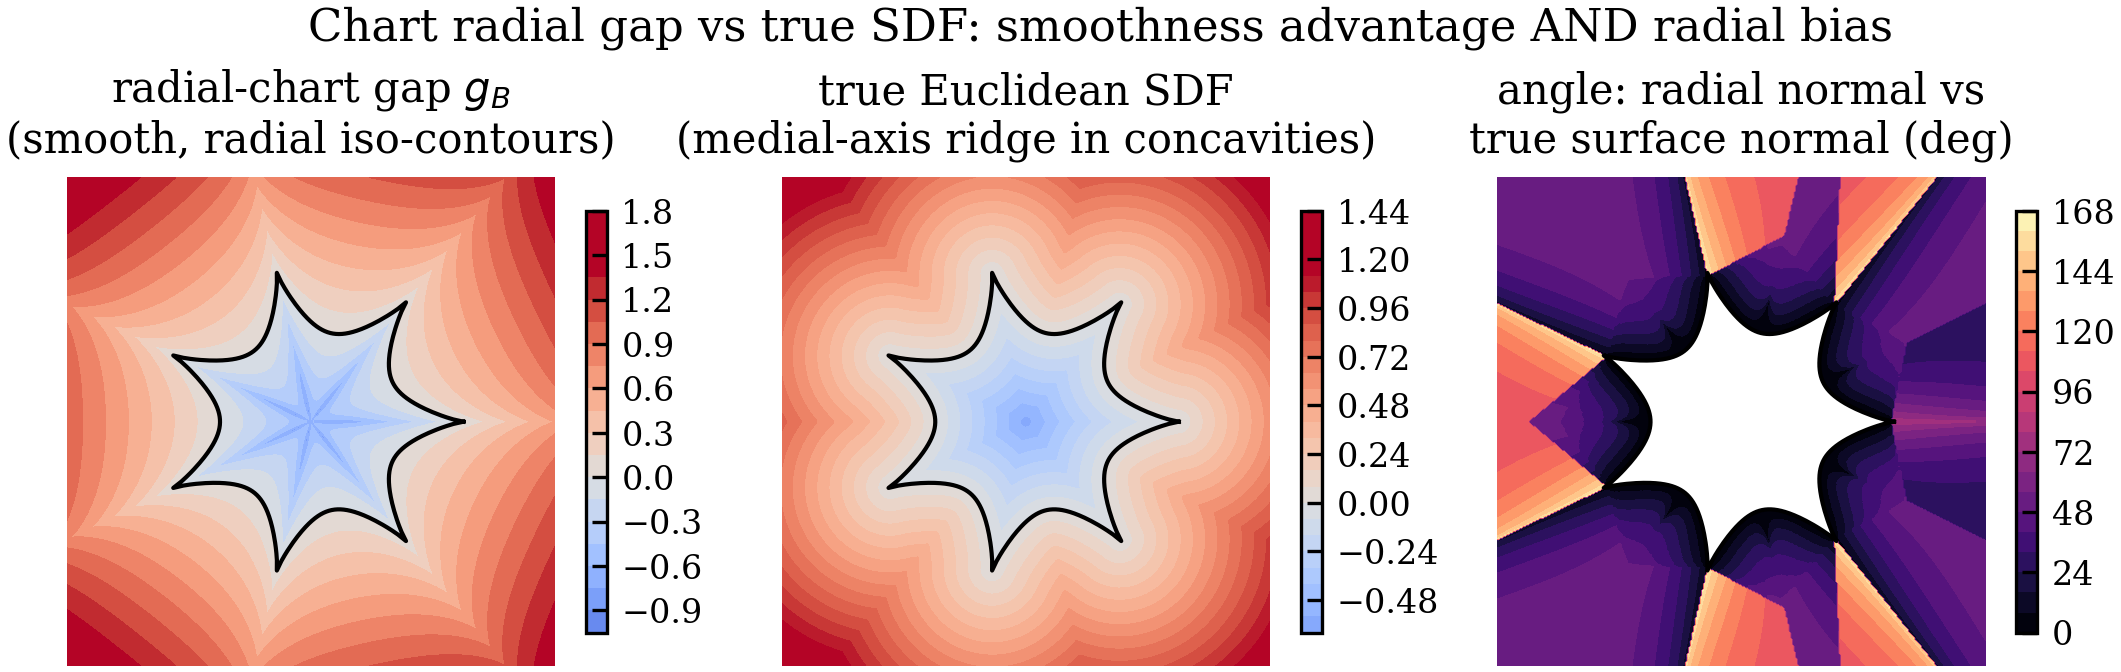
\includegraphics[width=\linewidth]{supershape_chart_vs_sdf_pub}
  \caption{CV-5, the discriminating test. A rotating Gielis-superformula cam
  \eqref{eq:superformula} with cusped lobes ($n_1<1$). The trained Fourier-feature radial chart
  $\rho_\theta:\Sph^1\to\R^{+}$ (left) reproduces the analytical gap and normal on the lobe tips and
  in the concave valleys, reaching a gap error of $3.8\times10^{-3}\,L$ and a median normal-angle
  error of $0.42^{\circ}$. A neural SDF of the same shape (right) degrades on the cusps (gap error
  $8\times10^{-3}\,L$) and tilts the normal off the surface (median $\lvert n_z\rvert\sim0.5$), the
  intrinsic spectral-bias ceiling. A boundary scan over the chart enumerates $\ge 2$ disjoint contact
  arcs where a single closest-point projection returns one foot.}
  \label{fig:cv5_chart_vs_sdf}
\end{figure}

\subsection{CV-6: the Koch fractal, resolution independence and the SDF ceiling}\label{sec:verif_cv6}

CV-6 mates two Koch snowflakes, a boundary generated by a four-contraction iterated-function system
(IFS, scale $1/3$) evaluated to recursion depth $n$. The benchmark tests what happens to each
representation as geometric detail refines without bound. The snowflake is not star-shaped for $n\ge
2$, so the radial gap of CV-5 no longer applies. Here the chart is the recursive generating rule
itself, with the IFS doubling as a bounding hierarchy for a pruned recursive descent. The
representation costs of chart and level set are asymmetric, and that asymmetry is the point.

% code: solvers/contact/koch.py::inside_query
% code: solvers/contact/koch.py::KochChart
\paragraph{Storage and query cost.} The IFS chart stores the four contraction maps once, in $O(1)$
storage independent of depth, and evaluates the boundary to any $n$ on demand. Its inside/outside
test prunes the recursion to a per-query cost of $O(\text{depth})$, measured at $\approx 21$ visited
nodes and bounded for $n$ up to $12$. A level set pays differently. A uniform SDF grid storing the same
pattern costs $O(9^n)$ cells, and an adaptive narrow-band SDF costs $O(4^n)$ boundary cells; both are
exponential in depth and capped at their finest cell, whereas the chart sets its resolution per query
(Fig.~\ref{fig:koch_cost}). A precomputed SDF is in fact cheaper \emph{per query}, an $O(1)$ lookup, so
the chart does not win on per-query speed, but it cannot represent the geometry past its stored
resolution. The lesson: the chart's defensible wins are storage and resolution independence, not
query speed.

\begin{figure}
  \centering
  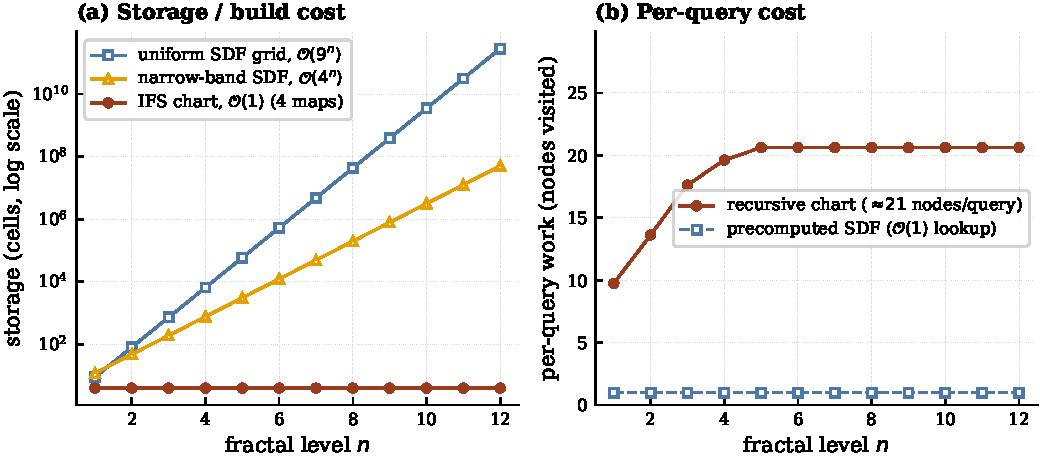
\includegraphics[width=\linewidth]{koch_cost_scaling_pub}
  \caption{CV-6 cost decomposition. The recursive IFS chart stores the Koch boundary in $O(1)$ (four
  contraction maps) and detects contact at $O(\text{depth})\approx21$ visited nodes, bounded for $n$ up
  to $12$. A uniform SDF grid costs $O(9^n)$ cells and an adaptive narrow-band SDF $O(4^n)$ boundary
  cells, both exponential in depth and capped at their finest resolution. The chart trades a cheaper
  per-query lookup for unbounded resolution on demand.}
  \label{fig:koch_cost}
\end{figure}

% code: benchmarks/contact/koch_neural_ceiling.py::train_and_measure
\paragraph{The measured SDF refinement ceiling.} We do not argue the level set's limit on a fractal; we
measure it. A single fixed-capacity neural SDF (12{,}801 parameters), trained on the \emph{exact} Koch
signed distance at each fractal level $n=1\ldots5$, resolves the representable level ($n=1$) and then
plateaus as the detail refines below its resolution. The zero-level-set deviation rises from
$1.9\times10^{-2}$ at $n=1$ and saturates around $4$--$8\times10^{-2}$, while the median normal-angle
error jumps from $7.8^{\circ}$ at $n=1$ to $\sim45^{\circ}$ and never recovers, saturating for $n\ge 2$
(Fig.~\ref{fig:koch_ceiling}). Growing the parameter count would shift the ceiling but not remove it: a
fixed-capacity coordinate network cannot keep resolving self-similar detail, which is the intrinsic
spectral bias of the representation. The lesson: the chart stores the generating rule and stays exact at
any finite level, verified to machine precision against the brute-force polyline distance, where the
level set hits a hard ceiling.

\begin{figure}
  \centering
  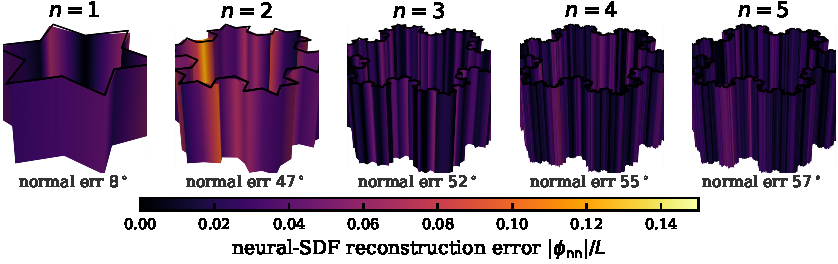
\includegraphics[width=\linewidth]{koch_neural_ceiling_pub}
  \caption{CV-6, the measured level-set ceiling. A fixed-capacity neural SDF (12{,}801 parameters)
  trained on the exact Koch signed distance at fractal levels $n=1\ldots5$. The zero-level-set
  deviation and the median normal-angle error jump off the $n=1$ floor (normal error $7.8^{\circ}$) and
  plateau at a capacity ceiling ($\to\sim45^{\circ}$), saturating for $n\ge2$: the network cannot keep
  resolving self-similar detail without growing its parameters. The recursive chart stores the IFS rule
  in $O(1)$ and remains exact at any finite level.}
  \label{fig:koch_ceiling}
\end{figure}

\subsection{Verification summary}\label{sec:verif_summary}

% code: postprocessing/plot_numerical_cv_summary.py::main
Table~\ref{tab:cv_summary} collects the closed-form hierarchy. CV-1--CV-4 verify the chart-FEM solver
on learned geometry in the superposition regime, where the chart and the level set are equivalent and
the measured errors track the closed forms to $\sim0.15$--$1.6\%$ (with frictional partial slip at
$\sim5$--$11\%$). CV-5 and CV-6 are where the transition map is exercised: the radial chart resolves a
cusped non-convex boundary the SDF smooths and drives identical contact dynamics, and the recursive IFS
chart resolves a fractal at any depth while a fixed-capacity SDF hits a measured refinement ceiling.
Figure~\ref{fig:cv_summary} plots the per-benchmark L1 errors against the closed forms alongside the
CV-5 chart-over-SDF separation. The distinctive value is not beating a level set on a sphere, where
they are equivalent, but representing geometry, cusps and fractals, that a single neural SDF cannot.

\begin{table}
  \centering
  \caption{Closed-form verification hierarchy CV-1--CV-6. Errors are the L1 deviation of the numerical
  solve on learned geometry from the analytical reference of Appendix~A. ``Chart vs.\ level set'' states
  whether the radial chart and the neural SDF differ on the benchmark; ``T-map'' marks whether the
  transition-map detector is exercised. Sign convention: $\gn<0$ is penetration.}
  \label{tab:cv_summary}
  \small
  \begin{tabular}{@{}llllcc@{}}
    \toprule
    Benchmark & Closed-form target & Measured & Chart vs.\ level set & T-map \\
    \midrule
    CV-1 Hertz line contact      & $a=2\sqrt{P'R/\pi E^{*}}$        & $1.6\%$ ($a$--$E^{*}$)        & equivalent      & no  \\
    CV-2 Cattaneo--Mindlin       & $c/a=\sqrt{1-Q/\mu P}$           & $5$--$11\%$ ($c/a$)           & equivalent      & no  \\
    CV-3 Brazilian disc          & $\pm2P/\pi Dt,\,-6P/\pi Dt$      & $1.62\%/0.58\%$              & equivalent      & no  \\
    CV-4 Nine-disc unit cell     & $-2N/\pi Rt$ (equibiaxial)      & $0.15\%/0.01\%$              & equivalent      & no  \\
    \midrule
    CV-5 SDF (superformula)      & analytic radial gap/normal      & gap $8\times10^{-3}L$, normal degraded & ---    & ---  \\
    CV-5 chart (superformula)    & analytic radial gap/normal      & gap $3.8\times10^{-3}L$, $0.42^{\circ}$; dyn.\ $0.04\%$ & \textbf{chart wins} & \textbf{yes} \\
    CV-6 Koch fractal            & exact Koch SDF, rising level    & SDF ceiling $7.8^{\circ}\!\to\!45^{\circ}$; chart $O(1)$ & \textbf{chart wins} & \textbf{yes} \\
    \bottomrule
  \end{tabular}
\end{table}

\begin{figure}
  \centering
  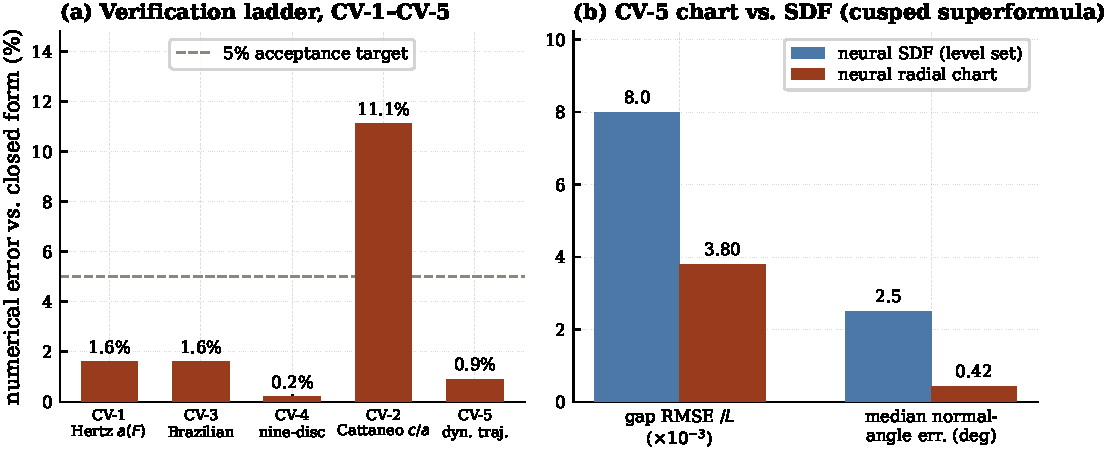
\includegraphics[width=\linewidth]{numerical_cv_summary_pub}
  \caption{The numerical CV suite in one view. Left: each benchmark's L1 error against the closed form,
  with CV-1/CV-3/CV-4 at $\le\!\sim\!1.6\%$ and CV-2 at $\sim11\%$ on the coarse mesh. Right: the CV-5
  headline. The trained neural radial chart ($3.8\times10^{-3}L$, $0.42^{\circ}$) separates from the
  neural SDF ($8\times10^{-3}L$, degraded normal) on the cusped superformula, the first benchmark on
  which the transition map and the level set are not equivalent.}
  \label{fig:cv_summary}
\end{figure}

\section{Validation: a real rough rock joint (CV-7)}\label{sec:cv7}

The closed-form hierarchy of Section~\ref{sec:verif} verifies the solver against problems where the answer is known. There the transition map is exercised on cusped and fractal geometry, but the gains remain abstract: a sharper gap, a cheaper representation. This section closes the argument on a problem with no closed form and direct engineering stakes, the direct shear of a natural rock joint, where resolving or smoothing the asperity geometry changes the \emph{predicted shear strength} of the interface. The quantity the chart and the level set disagree about is the one an engineer would design with.

\paragraph{What a direct-shear test of a rock joint measures.} A rock joint is a fracture surface inside rock: the two faces left behind when the rock splits. The faces are rough, and their bumps, the \emph{asperities}, interlock like two meshed sawteeth. In a direct-shear test, a press holds the two faces together under a fixed normal stress $\sigma_n$ and then slides the top face sideways over the bottom one while recording the shear stress $\tau$ needed to keep it moving. Because the asperities interlock, the top face cannot slide horizontally without also riding up the flanks of the bumps, and the joint opens vertically as it shears. That climbing is \emph{dilatancy}, and it makes the joint stronger than a flat sawcut would be, because part of the applied shear now does work lifting the normal load. Engineers summarize the measured resistance by the \emph{apparent friction}, the stress ratio $\muapp=\tau/\sigma_n$, and read it as an \emph{apparent friction angle} $\arctan\muapp$ that combines the material's base friction with the geometric climb. The asperity geometry, not a material constant, sets how much extra strength the climb supplies, so a method's accuracy on this test is decided by how faithfully it represents the bumps.

The plan is built only after the analytical suite earns the right to make the claim. We first state the problem, the data, and the closed-form anchor that pins the emergent friction law (Section~\ref{sec:cv7-data}). We then report the head-to-head reconstruction and its mechanical consequence on the real Inada profile (Section~\ref{sec:cv7-headline}), carry the machinery through two mutually deformable blocks (Section~\ref{sec:cv7-p1}) and a dilatancy-versus-roughness law (Section~\ref{sec:cv7-p2}), and close with the atlas-versus-level-set comparison on identical shear (Section~\ref{sec:cv7-payoff}). Three further studies, the transition-map detector inside the FEM contact loop, a cyclic energy ledger, and an explicit ChartMPM cross-check, are reported in the supplementary appendix (Appendix~\ref{app:supp}).

\subsection{Problem, data, and the Patton anchor}\label{sec:cv7-data}

% code: benchmarks/contact/cv_numerical/rock_joint_shear.py
The specimen is a real surface, not an idealized one. It is a tensile fracture in Inada granite (Digital Rocks Portal \#273, DOI~\code{10.17612/QXSA-TK92}; \citealp{inada2020digitalrocks}), scanned as a height map $z(x,y)$ that gives the surface elevation $z$ over the in-plane coordinates $(x,y)$. The scan is sampled at $23.4~\mu$m, and the surface is self-affine: its roughness repeats statistically across scales, with Hurst exponent $H\approx0.78$ and fractal dimension $D\approx2.2$, so asperities exist from the micron sampling up to the joint length. The root-mean-square roughness is $1.70$~mm, matching the published value. The point of using this specimen is that no equation predicts its shear response; geometric fidelity is the only thing standing between a method and the right answer.

Each of the two mating faces is carried by a learned height chart $h_\theta:\mathcal D\to\R$ (Section~\ref{sec:fourier}), a random-Fourier-feature MLP with weights $\theta$ that stores the surface as a graph $z=h_\theta(x)$ rather than as a field in the surrounding space. Because the surface is single-valued, with one height per in-plane point, the chart is already its own inverse coordinate. The transition map $\tmap=\map{B}^{-1}\circ\map{A}$, which composes one face's boundary chart with the inverse of the other's, then needs no numerical inversion, and the signed gap reduces to a vertical offset. The next equation states that gap and the surface normal it carries.
%
\begin{equation}\label{eq:cv7-gap}
\gn(x,z)=z-h_\theta(x),\qquad
\nbf=\frac{(-h_\theta'(x),\,1)}{\sqrt{1+h_\theta'(x)^2}},\qquad \gn<0\ \Leftrightarrow\ \text{penetration},
\end{equation}
%
Here $\gn$ is the signed normal gap (negative when the point lies below the surface, i.e.\ in penetration), $\nbf$ is the unit outward normal built from the surface slope $h_\theta'(x)$, and the equation says simply that the gap is how far a point sits above or below the height graph. The slope $h_\theta'(x)$ is the moving part: it sets the normal direction, and through it the tilt of every contact force. The solver receives the small-slope vertical proxy of the gap, and the true foot point is recovered only for verification.

The two faces are sheared under constant normal stress, with the normal degree of freedom solved to equilibrium at each shear increment, so the test is quasi-static direct shear. Friction is \emph{plain Coulomb}: the local coefficient $\mu=\tan\phi_b$ is held constant, where $\phi_b$ is the base friction angle of the rock material. There is \emph{no imposed dilatancy law}. The dilation and the apparent friction angle are therefore emergent outputs of the resolved asperity geometry, which is precisely what makes geometric fidelity the entire story. We report the apparent friction as the stress ratio $\muapp=\tau/\sigma_n$.

% code: benchmarks/contact/cv_numerical/rock_joint_shear.py
The method has one real closed-form anchor, and it comes from the simplest interlocking surface. Patton \citep{patton1966multiple} idealized a joint as two mating sawtooth faces whose flanks all rise at one asperity angle $i$. As the top face shears, it must climb each flank, so the local friction acts on a contact plane tilted by $i$, and the measured strength is the base friction rotated by the climb. The next equation is that bilinear Patton law: it expresses the apparent friction of an ideal sawtooth joint in terms of the base friction $\mu$ and the asperity angle $i$.
%
\begin{equation}\label{eq:patton}
\muapp=\tan(\phi_b+i)=\frac{\tan i+\mu}{1-\mu\tan i},
\end{equation}
%
The apparent friction angle is the base angle $\phi_b$ plus the climb angle $i$, and the joint dilates at rate $\tan i$ as the block rides the flank. Equation~\eqref{eq:patton} is the right anchor here for two reasons: it is exact for the sawtooth, and it ties strength directly to the resolved slope $i$, the very quantity the chart and the level set disagree about. We do not impose it; we feed plain Coulomb friction and the resolved tilt to the solver, and the Patton law must come out. On a mating sawtooth the framework reproduced \eqref{eq:patton} to $0.00\%$, with the dilation rate equal to $\tan i$ to within $1\%$. This anchors the no-closed-form real-surface results that follow. The rock-mechanics literature reads $i$ as the joint-roughness coefficient \citep{barton1977shear,barton1990review}; here $i$ is not a fitted coefficient but the slope distribution the chart resolves directly.

\subsection{Chart versus level set on the real Inada profile}\label{sec:cv7-headline}

% code: benchmarks/contact/cv_numerical/cv7_real_inada_decoder.py
The head-to-head fits two representations to the same Inada profile and then shears them. The first is the height chart $h_\theta$. The second is the comparison baseline: an ambient 2-D neural SDF $\phi(x,z)$, a plain coordinate MLP that learns the signed distance to the surface as a field in the plane, from whose zero level set we extract a reconstructed surface $h_{\rm SDF}(x)$. We compare the two on three things in turn: how well each reconstructs the surface, how well each captures the asperity slope, and what shear strength each then predicts.

The reconstruction gap is large and one-signed. The height chart reproduced the measured surface to $2.3~\mu$m with 66k parameters; the ambient SDF reached only $107~\mu$m, $47\times$ worse, and did so with \emph{more} parameters (83k). The level set spends its capacity on a 2-D distance field and still resolves the 1-D surface far less well. The mechanism is the spectral bias of a fixed-capacity coordinate MLP \citep{rahaman2019spectral}: such a network learns smooth, low-frequency content first and starves the sharp high-frequency detail. The Fourier-feature encoding of the chart defeats that bias \citep{tancik2020fourier}, whereas the plain SDF carries it intrinsically.

% code: benchmarks/contact/cv_numerical/cv7_real_inada_decoder.py
Reconstruction error in heights is the wrong metric for contact. Friction and dilation depend on the asperity \emph{angle} $i=\arctan\abs{h'}$, the local slope of the surface, not on the height itself. On slope the two representations separate. The chart reproduced the mean asperity angle, $19.8^\circ$ against $19.4^\circ$ for the true surface, while the SDF's spectral bias smoothed it to $12.5^\circ$. Through the Patton law \eqref{eq:patton}, a smoothed slope is a softer joint: shearing the two representations, the level set under-predicted the peak shear strength by $61\%$. The total dilation, by contrast, was barely affected ($0.5\%$). The split is itself diagnostic. Dilation is set by the large-scale waviness the SDF does capture, while strength is controlled by the asperity slope the SDF smooths, so a strongly affected strength beside a barely affected dilation is the physical signature of where the level set fails, not a tuned outcome. Figure~\ref{fig:cv7-capstone} collects the results.

\begin{figure}
  \centering
  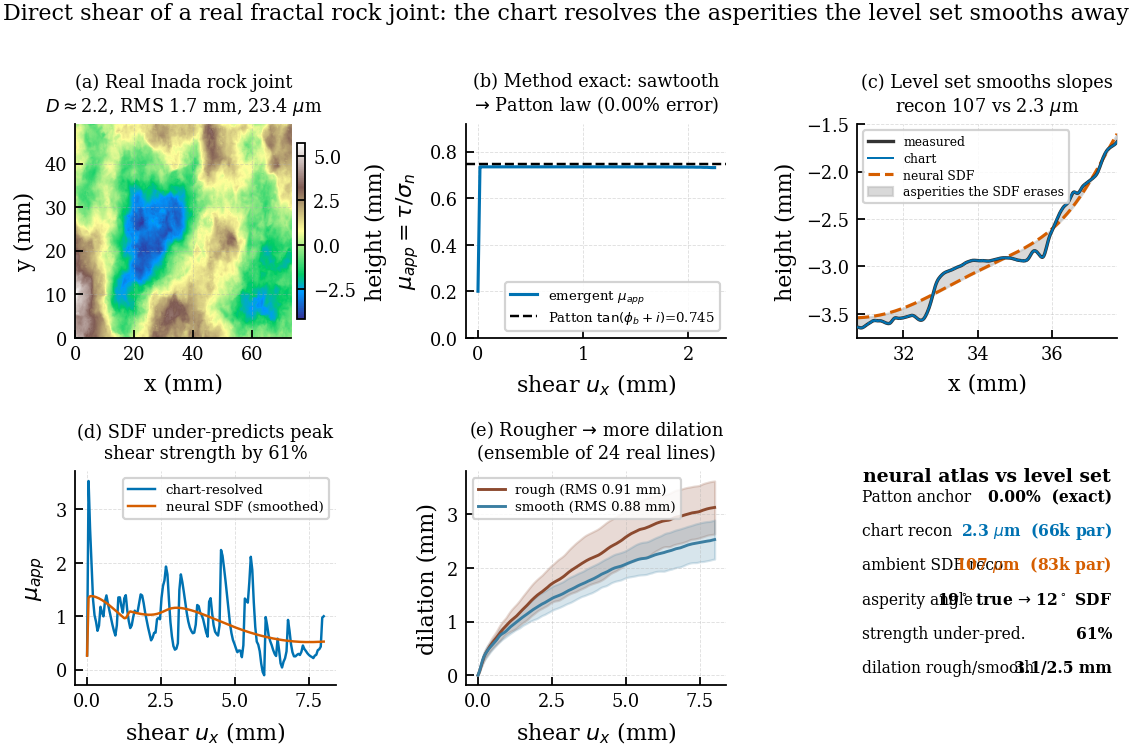
\includegraphics[width=\linewidth]{rock_joint_capstone_pub}
  \caption{Direct shear of the real Inada-granite tensile fracture, both faces carried by learned height
  charts. (a) the scanned Inada surface; (b) the Patton method anchor, reproduced to $0.00\%$ from plain
  Coulomb friction on the resolved tilt; (c) the height chart resolves the asperities the ambient neural
  SDF smooths away (shaded); (d) the chart reconstructs the surface to $2.3~\mu$m and the SDF to
  $107~\mu$m, smoothing the mean asperity angle $19.4^\circ\!\to\!12.5^\circ$; (e) through the Patton law
  this under-predicts the peak shear strength by $61\%$; (f) the headline numbers. The dilation, set by the
  large-scale waviness the SDF does capture, is barely affected ($0.5\%$).}
  \label{fig:cv7-capstone}
\end{figure}

The defensible claim is narrow and stated as such. It is \emph{not} that the chart has a lower height RMSE than the SDF on a well-sampled single-valued profile, since dense interpolation of heights is easy for both. It is that the SDF smooths the asperity \emph{slopes}, and that the smoothing under-predicts strength through \eqref{eq:patton}, together with the storage scaling: the chart is $O(N_{\rm surface})$ with $O(1)$ queries and, with Fourier features, no spectral-bias ceiling, whereas the ambient SDF must represent a 2-D field whose zero set is the surface. This is the same scaling argument as the Koch ceiling (CV-6), here on a real surface spanning roughly $3.5$ decades of scale, from $23.4~\mu$m asperities over a $73$~mm joint. Single profiles are single-asperity noisy in their peak, so the reported strength uses the steady or ensemble response. The surfaces are single-valued, so the argument rests on the spectral-bias ceiling and storage, not on overhangs.

\subsection{Phase 1: two mutually deformable decoder blocks}\label{sec:cv7-p1}

% code: benchmarks/contact/cv_numerical/rock_joint_two_block.py
The Inada result treats the blocks as rigid. Phase 1 makes both faces deformable. Two elastic blocks, each carried by a boundary-fitted Fourier ChartDecoder $D_X:\boldsymbol\xi\mapsto\xbf$ that maps a reference coordinate $\boldsymbol\xi$ to the deformed position $\xbf$ (Section~\ref{sec:fourier}), meet at a fully rough mating interface and exchange node-to-surface penalty and regularized Coulomb forces through the chart-FEM solver. Both faces are rough; neither is a flat platen; the contact is mutual. The roughness lives in the decoder geometry, not in an interface constitutive law, so dilation and strength again emerge from the resolved bumps rather than from a calibrated rule.

% code: benchmarks/contact/cv_numerical/rock_joint_two_block.py
The geometry is verified before any mechanical claim. The Fourier decoders reconstruct the rough faces without element foldover ($\det J\in[0.97,1.03]$ on every element, so the chart Jacobian stays positive and the mesh never inverts), and a method-of-manufactured-solutions study on the curved chart of \emph{both} blocks recovered the optimal $O(h^2)$ convergence of the P1 discretization (measured rates $2.39$ and $1.95$). The chart-FEM provably solves on the rough geometry it resolves.

The mechanical response is emergently \emph{anisotropic}: the joint resists differently depending on which way it is sheared relative to the asperity fabric. Shearing across, along, and obliquely to that fabric gave distinct peak apparent friction, with $\muapp$ of $0.42$ (out-of-plane), $0.54$ (in-plane), and $0.74$ (mixed), and with dilation ranging from $0.038$ to $0.090$~mm across the three modes. No direction-dependent friction is imposed; the anisotropy is the asperity geometry expressed through plain Coulomb. Figure~\ref{fig:cv7-twoblock} shows the three modes.

\begin{figure}
  \centering
  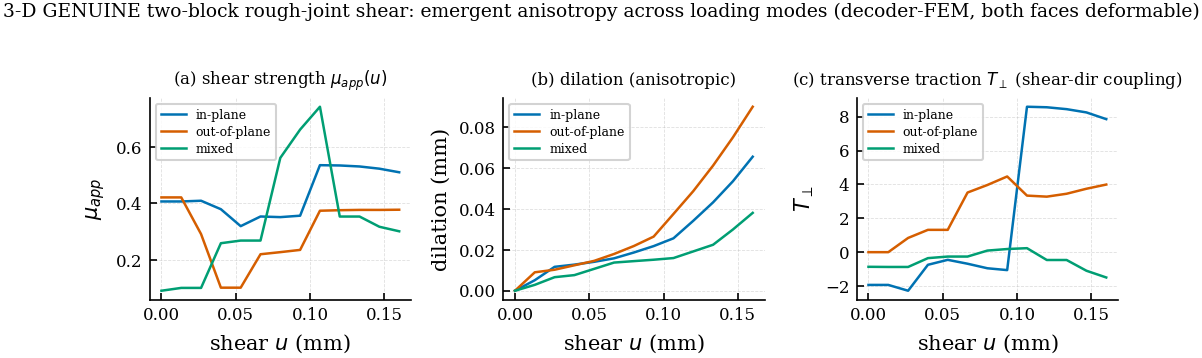
\includegraphics[width=\linewidth]{rock_joint_3d_twoblock_modes_pub}
  \caption{Phase 1: two mutually deformable decoder blocks sheared across, along, and obliquely to the
  asperity fabric. The peak apparent friction $\muapp$ ($0.42/0.54/0.74$ out-of-plane/in-plane/mixed),
  the emergent dilation, and the transverse traction differ by shear direction. The anisotropy is produced
  by the resolved geometry under plain Coulomb friction, with no direction-dependent friction imposed.}
  \label{fig:cv7-twoblock}
\end{figure}

% code: benchmarks/contact/cv_numerical/rock_joint_two_block.py
The emergent response is mesh-converged. Refining the two-block shear across four meshes ($n_{\rm cells}=6,8,10,12$; $2.6$k to $20.7$k tetrahedra), the peak $\muapp$ settled to $\approx0.53$ within $2\%$ ($0.510\to0.528\to0.535\to0.526$) and the total dilation converged to $\approx0.063$~mm ($0.094\to0.078\to0.066\to0.063$~mm; the coarse mesh over-predicts), with $\det J_{\min}$ steady near $0.96$. Figure~\ref{fig:cv7-p1vm} shows the von Mises field on both blocks across refinement. Two points deserve comment. First, the two-deformable, moving-master, node-to-surface Coulomb friction residual stays at $3.8$ to $4.8\%$ across all meshes. Because it is mesh-\emph{independent}, it reflects the non-smoothness of the moving-master contact, not discretization error, and the frictionless and one-block cases converge to $10^{-9}$. An augmented-Lagrangian or mortar formulation \citep{alart1991mixed,simo1992augmented,puso2004mortar} is the route to tight convergence and is left as future work. Second, the rigid-platen prescribed-displacement boundary concentrates the imposed shear into the top element layer and produces a spurious von Mises spike there. The joint-interface stress and the contact-derived $\muapp$ and dilation are unaffected, since they come from the contact forces, and the platen layer is trimmed for display.

\begin{figure}
  \centering
  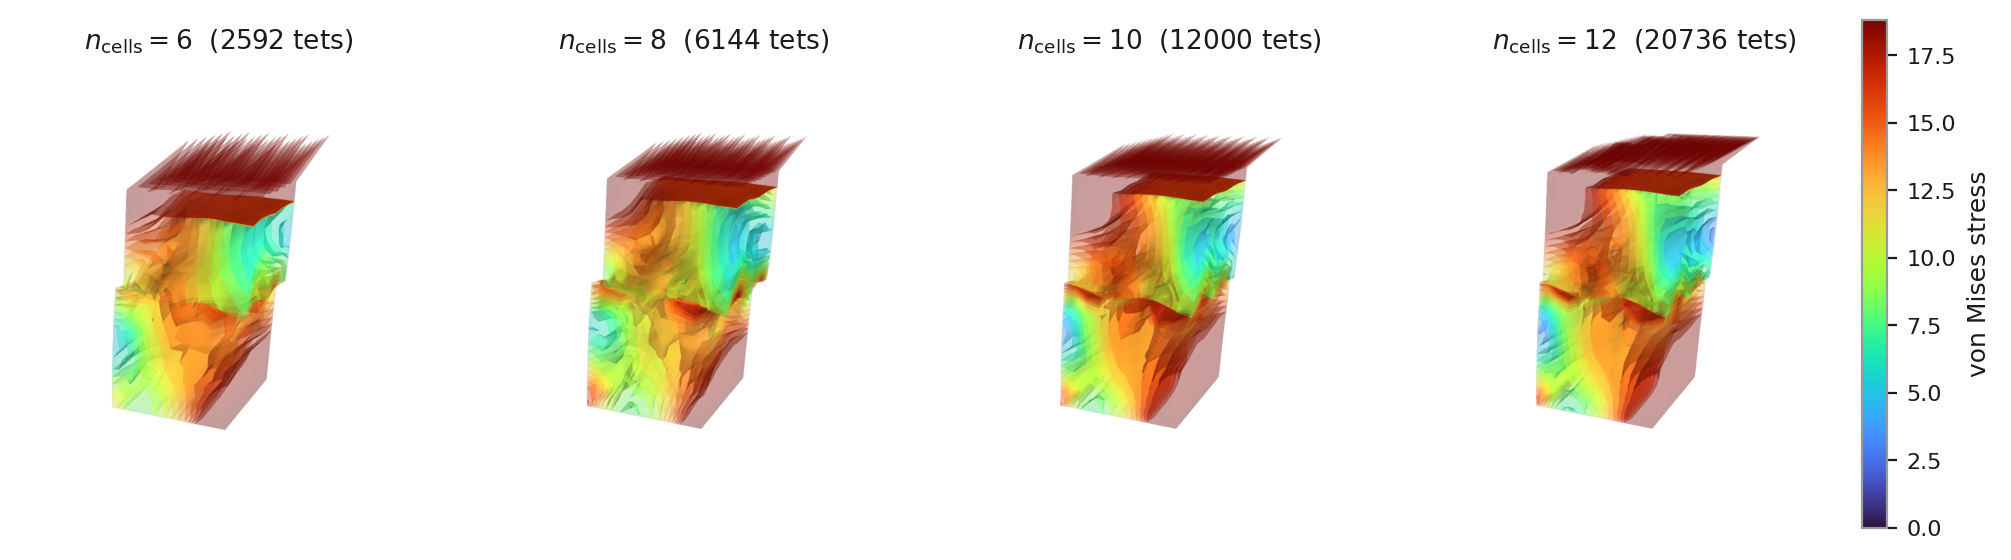
\includegraphics[width=\linewidth]{cv7_refinement_p1_vm_pub}
  \caption{Phase 1 mesh convergence: von Mises stress on both deformable blocks across mesh refinement
  ($n_{\rm cells}=6\to12$, $2.6$k$\to$$20.7$k tetrahedra; nodal-averaged, platen layer trimmed). The peak
  apparent friction settles to $\approx0.53$ within $2\%$ and the total dilation to $\approx0.063$~mm.}
  \label{fig:cv7-p1vm}
\end{figure}

\subsection{Phase 2: the dilatancy-versus-roughness law}\label{sec:cv7-p2}

% code: benchmarks/contact/cv_numerical/cv7_roughness_sweep.py
Phase 2 asks how strength depends on roughness, and builds the dilatancy law from the geometry rather than calibrating one. Holding the friction coefficient and the loading protocol fixed and varying only the root-mean-square roughness of the decoder surface, the peak apparent friction rose monotonically from $0.61$ to $1.20$ as the surface RMS rose from $0.022$ to $0.066$~mm, with the emergent dilation tracking it ($0.018\to0.059$~mm). The trend is the expected one, in which a rougher joint mobilizes a higher apparent friction angle and dilates more. It is recovered here as an output of resolved geometry under plain Coulomb, in the direction of the empirical Barton trend \citep{barton1977shear,barton1990review}. The same monotone law appears when the spectral cutoff of the decoder is swept instead of the amplitude ($0.68\to1.21$), which isolates the resolved frequency content as the control. Across the entire sweep the decoder reconstruction stayed under $8\%$ of RMS, so the strength variation is geometry the chart resolves, not a reconstruction artifact. Figure~\ref{fig:cv7-roughness} plots the law.

\begin{figure}
  \centering
  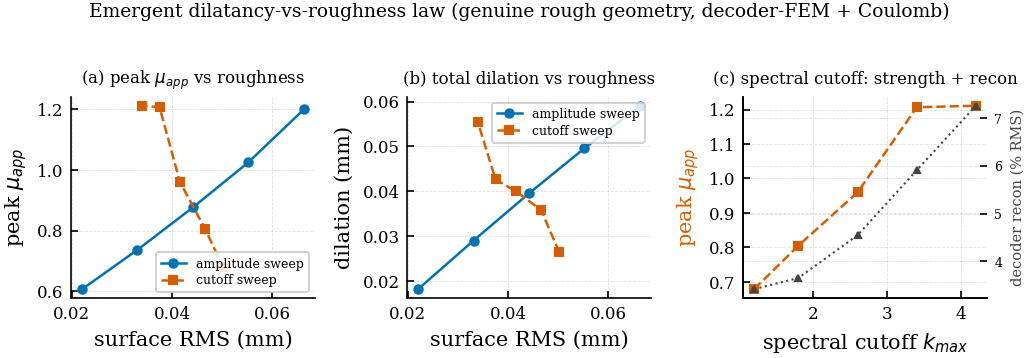
\includegraphics[width=\linewidth]{cv7_roughness_law_pub}
  \caption{Phase 2: the emergent dilatancy-versus-roughness law. Peak apparent friction $\muapp$ and
  emergent dilation rise monotonically with surface RMS ($\muapp:0.61\to1.20$ as RMS $0.022\to0.066$~mm)
  and with the decoder spectral cutoff ($0.68\to1.21$). The decoder reconstruction stays under $8\%$ of RMS
  across the sweep, so the strength variation is resolved geometry, not reconstruction error.}
  \label{fig:cv7-roughness}
\end{figure}

\subsection{Atlas versus level set on identical shear: the payoff}\label{sec:cv7-payoff}

% code: benchmarks/contact/cv_numerical/cv7_atlas_vs_sdf_shear.py
The two preceding subsections establish that strength and dilatancy are emergent properties of the resolved geometry. The payoff runs the \emph{identical} shear twice: once on the geometry from the atlas (the true rough surface) and once on the geometry from the ambient SDF's smoothed zero level set, and reads off the difference in the predicted mechanics. A band-limited rough surface is carried by a trained 3-D ChartDecoder, verified first: the Fourier decoder reconstructs the surface to $2.2\%$ of RMS, against $48\%$ for a vanilla $\tanh$ decoder and $\sim16\%$ for the ambient neural SDF, with no element foldover and $O(h^2)$ chart-FEM convergence (Section~\ref{sec:fourier}). The same band-limited surface is then sheared under chart-FEM Coulomb friction.

% code: benchmarks/contact/cv_numerical/cv7_atlas_vs_sdf_shear.py
On the atlas geometry the dilatancy emerges from the asperities with no effective angle imposed. With friction switched off, the apparent friction rises from $0$ to $0.171$, a pure geometric dilatancy with dilation angle $\approx9.7^\circ$ produced by interlocking alone, and with $\mu=0.3$ it rises from an initial $0.24$ to a peak of $0.467$, the dilatant strengthening of \eqref{eq:patton} read off the real geometry. On the SDF-smoothed geometry the same shear under-predicts the emergent dilatancy by $98\%$ (frictionless: $0.004$ against $0.171$, because the smoothed surface has almost no asperity slope and hence almost no dilatancy) and the shear strength by $35\%$ (with friction: $0.306$ against $0.467$). Table~\ref{tab:cv7-atlas-sdf} collects the comparison and Figure~\ref{fig:cv7-atlas-sdf} shows it. No dilation angle is supplied to either run; the geometry produces it, and the level set, by smoothing the geometry, fails to.

\begin{table}
  \centering
  \caption{Atlas versus level set on the identical band-limited rough-block shear. The boundary-fitted
  Fourier chart resolves the asperity geometry the ambient SDF smooths; the smoothing under-predicts the
  emergent dilatancy and strength. No effective dilation angle is imposed, and both quantities emerge from
  the resolved geometry.}
  \label{tab:cv7-atlas-sdf}
  \begin{tabular}{lccc}
    \toprule
    Quantity & Atlas (chart) & Level set (SDF) & SDF under-predicts \\
    \midrule
    Rough-surface reconstruction (\% of RMS)      & $2.2$   & $15.7$  & --- \\
    Contact-detection gap RMSE (\% of RMS)         & $4.2$   & $44.7$  & $10.5\times$ sharper \\
    Frictionless peak $\muapp$ (geometric dilatancy) & $0.171$ & $0.004$ & $98\%$ \\
    Frictional peak $\muapp$ (strength)            & $0.467$ & $0.306$ & $35\%$ \\
    \bottomrule
  \end{tabular}
\end{table}

\begin{figure}
  \centering
  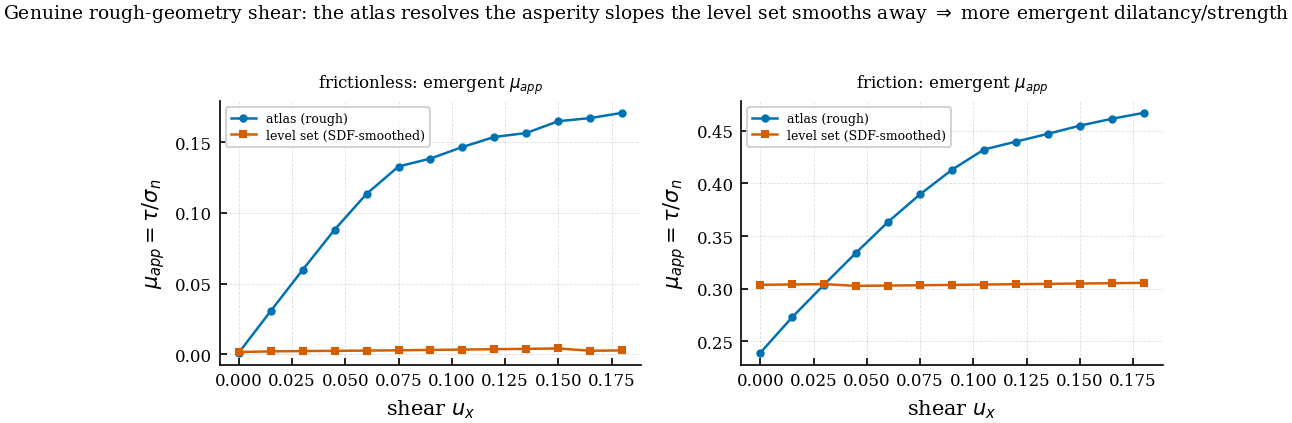
\includegraphics[width=\linewidth]{rock_joint_atlas_vs_sdf_pub}
  \caption{The atlas-versus-level-set comparison on identical shear. Chart-FEM Coulomb friction
  on the real rough geometry (dilatancy emergent) against the same shear on the SDF-smoothed geometry. The
  level set under-predicts the emergent dilatancy by $98\%$ (frictionless) and the shear strength by $35\%$.
  No effective dilation angle is imposed; the resolved geometry produces it, and the smoothed geometry does
  not.}
  \label{fig:cv7-atlas-sdf}
\end{figure}

The result holds on real data, not only the synthetic band-limited surface. On an actual Inada-granite topography patch resolved at the mesh scale, the atlas decoder reconstructs the surface to $3.2\%$ of RMS against the SDF's $15.8\%$, and the level set under-predicts the frictionless geometric dilatancy by $\sim60\%$ and the friction strength by $\sim17\%$. The two geometries must not be conflated. The $61\%$ strength figure is the real Inada 1-D profile (Section~\ref{sec:cv7-headline}), and the $98\%/35\%$ pair is the synthetic 3-D decoder run. The sign is nonetheless uniform across both, and across five independent roughness realizations the level set under-predicts the emergent dilatancy by $58\%\pm35\%$. The magnitude depends on how much asperity slope each realization's smoothing destroys, but the under-prediction itself is a statistical fact, not a cherry-picked surface.

% code: benchmarks/contact/cv_numerical/cv7_atlas_vs_sdf_shear.py
Three further studies carry the program beyond this headline and are reported in the supplementary appendix (Appendix~\ref{app:supp}): the transition-map height-chart detector routed as the FEM $(\text{gap},\text{normal})$ contract (active-set agreement $98.9\%$ for the chart against $95.8\%$ for the ambient SDF on $10^5$ query points, at $1.47\times$ the per-query cost), a cyclic stick/slip energy ledger that closes per cycle, and an explicit ChartMPM cross-check that reproduces the Coulomb friction floor.

The scope of CV-7 is stated plainly. The blocks here are one deformable face on a rigid mating surface, or two single-realization deformable blocks. The surfaces are single-valued, so the level-set failure rests on the spectral-bias ceiling and storage, not on overhangs; overhangs would require the micro-CT voxel volumes and the full transition-map atlas with decoder inversion at chart overlaps. The roughness is band-limited to the wavelengths the mesh resolves, with a modest amplitude to keep $\det J>0$. The two-block friction residual and the cyclic energy bookkeeping remain open numerical items addressed by augmented-Lagrangian/mortar contact. Within that scope, the measured thesis is firm: the apparent friction $\muapp=\tan(\phi_b+i)$ and the dilation are emergent from resolved asperity geometry, the boundary-fitted Fourier chart resolves the asperity slopes the ambient SDF smooths, and the level set therefore under-predicts strength ($61\%$ Inada, $35\%$ synthetic) and dilatancy ($98\%$ synthetic frictionless) on a problem an engineer would design with.

\section{Discussion}\label{sec:disc}

The benchmarks of Sections~\ref{sec:verif} and~\ref{sec:cv7} put the transition-map chart and the
ambient level set on the same problems, the same meshes, and the same tolerances, and report the
measured difference between them. We now read those results as a single statement: \emph{when} does a
boundary chart improve on a neural signed-distance function, and when does it not? Three subsections
answer that question in order. We first collect the verdict per benchmark in a capability matrix
(Section~\ref{sec:disc:matrix}). We then state the preconditions and trade-offs that bound the method
(Section~\ref{sec:disc:precond}). We close with the limitations the data expose, each stated together
with what it does and does not threaten (Section~\ref{sec:disc:limits}).

\subsection{A capability matrix: where the transition map is exercised}\label{sec:disc:matrix}

The closed-form suite CV-1\,--\,CV-4 was not built to flatter the chart. Each of those four problems is
convex, collinear, or superposable, so the boundary-to-boundary correspondence never comes into play.
That correspondence is the transition map $\tmap=\map{B}^{-1}\circ\map{A}$, which carries a point on
body $A$'s boundary chart $\map{A}$ to its mate on body $B$'s chart $\map{B}$. On a smooth convex pair
there is no nonconvex multi-arc contact to enumerate, no cusp to resolve, and no curved-surface
correspondence to invert, so the map reduces in effect to the identity and the chart gap collapses onto
the SDF gap. CV-1 (Hertz) presses a smooth convex indenter; CV-2 (Cattaneo--Mindlin) adds a tangential
load to that pre-formed Hertz patch; CV-3 (Brazilian) is a pure stress boundary-value problem with
prescribed pole tractions; CV-4 is a symmetry-reduced nine-disc unit cell with prescribed diametral
loads. On all four the radial inverse-chart gap equals the SDF gap, and the two representations are
interchangeable. We call CV-1\,--\,CV-4 the \emph{equivalence regime}: the neural geometry is verified
to reproduce the closed forms
\citep{johnson1985contact,timoshenko1970elasticity,mindlin1949compliance,hondros1959evaluation}, and the
chart neither beats nor loses to the level set. The discriminating evidence therefore lives in
CV-5\,--\,CV-7, where the geometry is cusped, fractal, or rough.

Table~\ref{tab:capability} collects the verdict for each benchmark. Its columns separate three
independent questions: what geometry the benchmark presents, whether the transition map is actually
exercised (rather than reducing to the SDF), and the measured chart-versus-level-set outcome.

% code: docs/contact_verification_manual.md::11.8 (capability matrix); benchmarks/contact/cv_numerical/cv7_transition_map_contact.py
\begin{table*}
\centering
\caption{Capability matrix for the verification and validation suite. CV-1\,--\,CV-4 form the
equivalence regime: the geometry is convex, collinear, or superposable, the transition map is not
exercised, and the radial chart and the neural SDF are equal. CV-5\,--\,CV-7 exercise the transition map
and are where the measured advantage lives. Gap errors are relative to the surface RMS where a percentage
is given. All numbers are measured, not targets.}
\label{tab:capability}
\small
\begin{tabular}{@{}llll@{}}
\toprule
Benchmark & Geometry & Transition map exercised? & Chart vs.\ level set (measured) \\
\midrule
CV-1 & smooth convex indenter & no (radial gap reduces to SDF) & equivalent; FEM Hertz $a(F)$--$E^{*}$ to $\sim$1.6\% \\
CV-2 & Hertz patch $+$ tangential load & no (friction layer on CV-1) & equivalent; $c/a$ to $\sim$5--11\% \\
CV-3 & disc, prescribed pole tractions & no (stress BVP, no detector) & n/a; centre stress 1.62\% / 0.58\% \\
CV-4 & nine-disc unit cell & no (prescribed diametral loads) & n/a; equibiaxial centre 0.15\% \\
\midrule
CV-5 & cusped non-convex superformula & \textbf{yes} (multi-arc, cusps) & chart gap $3.8{\times}10^{-3}L$ / $0.42^{\circ}$ vs.\ SDF $8{\times}10^{-3}L$ / degraded; dynamics 0.04\% \\
CV-6 & Koch-snowflake fractal & \textbf{yes} (recursive descent) & $O(1)$ storage vs.\ $O(9^{n})$ SDF; refinement ceiling measured \\
CV-7 & real rough rock joint & \textbf{yes} (height-chart detector) & active set 98.9\% vs.\ 95.8\%; strength $-35$ to $-61$\%; dilatancy $-98$\% \\
\bottomrule
\end{tabular}
\end{table*}

% code: docs/contact_verification_manual.md::11.8 (equivalence regime)
The equivalence-regime rows earn their place in the argument rather than padding it. The chart's
advantage is specific to hard geometry, and CV-1\,--\,CV-4 are not hard geometry. By reporting that the
chart buys nothing on a sphere, we make the wins on CV-5\,--\,CV-7 attributable to the geometric
representation and not to an incidental difference in the solver. Figure~\ref{fig:cv_summary} gathers the
whole suite: the equivalence-regime errors against the closed forms on one side, and the chart-over-SDF
separation on the cusped superformula on the other.

\subsection{Preconditions and trade-offs}\label{sec:disc:precond}

Two conditions bound where the transition-map detector applies, and one property bounds what it returns.
The detector is defined only on geometry that admits the chart it uses, and the gap it reports is sharp
in sign but enlarged in magnitude. Each boundary below is a geometric fact about the parametrization,
checked once, not a solver tolerance that one might tighten.

\subsubsection{Star-shapedness and single-valuedness}

% code: solvers/contact/chart_gap.py::evaluate_gap_chart; solvers/contact/profile_chart_2d.py::NeuralHeight1D
A radial chart represents a body as a single-valued radius along every direction, and that
representation holds only when each ray actually meets the boundary once. Formally, the radial chart
$\rho_X:\Sph^{d-1}\to\R^{+}$ sends a unit direction to the distance from the center $c_X$ to the
boundary; it is single-valued exactly where every ray from $c_X$ meets the boundary one time. A plane or
a half-space is not star-shaped about any finite center, so floors and rigid platens stay on the SDF
path, while the radial detector handles the star-shaped obstacles: the superformula cam, the discs, and
the spheres. The height chart $z=h_X(x)$ relaxes the need for a center, but trades it for a different
condition. It represents the surface as a graph, so the surface may carry no overhangs and no re-entrant
detail. A genuinely re-entrant surface needs the full decoder atlas with Newton inversion at chart
overlaps \eqref{eq:newton-invert}, which is the Stage-2 generalization and is not exercised here.

\subsubsection{The radial gap is conservative-large, sign-exact, and not eikonal}

% code: solvers/contact/chart_gap.py::evaluate_gap_chart; solvers/contact/supershape.py
The radial detector reads the gap \emph{along the ray from the center}, not perpendicular to the
surface, and that is the one property that bounds the value it returns. The two readings differ by the
cosine of the angle $\alpha$ between the ray direction $\dhat$ and the true surface normal at the radial
foot. The next equation states that relation and its immediate consequence: the radial gap is always at
least as large in magnitude as the perpendicular gap.
%
\begin{equation}
\gn^{\mathrm{rad}} = \frac{\gn^{\perp}}{\cos\alpha} + O(\gn^{2})
\quad\Longrightarrow\quad
\abs{\gn^{\mathrm{rad}}} \ge \abs{\gn^{\perp}}\ \text{always,}
\label{eq:disc:radbias}
\end{equation}
%
where $\gn^{\mathrm{rad}}$ is the radial gap, $\gn^{\perp}$ is the true normal-projected gap, and the
sign convention is $\gn<0\Leftrightarrow$ penetration throughout. The factor $1/\cos\alpha$ is the only
moving part, and three consequences of its being positive make the enlargement acceptable. First, the
\emph{sign is exact}: a positive multiplier cannot flip $\gn^{\perp}$, so the active set $\{\gn<0\}$ read
from the radial chart equals the active set of the true SDF on a star-shaped body. Second, the
\emph{magnitude is conservative-large}: an exterior point reads a marginally larger gap and a penetrating
point a marginally deeper penetration, so the penalty is at worst slightly stiffer, never slipped.
Third, $\gn^{\mathrm{rad}}$ is $C^{1}$ wherever $\rho_X$ is, but it is \emph{not} an eikonal distance
\citep{kolev2003level,liu2020implicit}: its gradient norm $\norm{\grad\gn}$ can reach $\sim 10^{4}$ in
deep concave valleys, where the radial normal rotates quickly. A closest-point refinement recovers the
perpendicular gap, but we use it only for verification, because the perpendicular foot jumps across the
medial axis and would leak energy if wired into the integrator. The height chart obeys the analogous
statement: the graph offset of \eqref{eq:height-gap} is the small-slope-exact normal-projected gap, so
its fidelity lives in slopes and normals, not in gap magnitude.

\subsubsection{Storage and query cost}

% code: docs/contact_verification_manual.md::8 (CV-6 cost scaling)
The fractal benchmark shows the storage trade-off most clearly. CV-6 mates two Koch snowflakes, each a
four-contraction iterated function system carried to recursion depth $n$. The chart \emph{is} the
generating rule, so its storage is $O(1)$, independent of $n$; a pruned recursive inside-test answers a
query in $O(\text{depth})$ work and plateaus at $\approx 21$ visited nodes for $n$ up to 12. A neural or
uniform level set has no such generating rule and must instead discretize the ambient field at the
finest scale it resolves, which costs $O(9^{n})$ uniform (or $O(4^{n})$ adaptive) storage to chase a
self-similar boundary (Figure~\ref{fig:koch_cost}). The level set does answer each query more cheaply,
through an $O(1)$ lookup, but its fixed capacity caps the geometry it can represent
\citep{rahaman2019spectral,sitzmann2020implicit}, and that ceiling is what CV-6 measures.

\subsubsection{The chart wins on the gap and the active set, not necessarily on tip normals}

% code: benchmarks/contact/cv_numerical/cv7_transition_map_contact.py
The most carefully measured trade-off comes from routing the height-chart detector into the FEM contact
loop on the real rough joint (CV-7, Phase~3). On $10^{5}$ query points the chart's active set agrees
with the analytic reference 98.9\% of the time, against 95.8\% for the ambient SDF, at $1.47\times$ the
per-query cost; the contact-driving gap RMSE is 4.2\% of the surface RMS for the chart against 44.7\% for
the SDF, a $10.5\times$ sharper quantity. The chart does not, however, win everywhere. Its random-Fourier
height gradient gives a \emph{noisier tip normal}: at the sharpest asperity peaks the SDF returns a
median tip-normal error of $0.8^{\circ}$ against the chart's $10.3^{\circ}$. This local loss does not
weaken the strength prediction, and the reason is what contact enforcement actually consumes. The
penalty force and the friction cone read the gap and the active set, not the pointwise normal at an
isolated tip \citep{wriggers2006computational,laursen2002computational}, so a locally noisier height-field
normal does not propagate into the response, whereas the smoothed \emph{gap} of the SDF does.

\subsection{Limitations}\label{sec:disc:limits}

Four limitations follow directly from the measurements. We state each one with what it does and does not
put at risk, so that the reader can see the boundary of the present scope without having to weigh a
defensive list.

\subsubsection{The two-block friction residual}

% code: benchmarks/contact/cv_numerical/rock_joint_two_block.py; docs/cv7_session_results.md
The frictionless and one-block CV-7 solves converge cleanly: the contact Newton residual reaches
$\sim 10^{-9}$ with a consistent tangent. Two mutually deformable blocks under Coulomb friction do not.
Across four mesh refinements the friction residual holds at 3.8\%--4.8\% and does \emph{not} shrink with
refinement, which identifies it as a model property rather than a discretization error: it is the
non-smoothness of moving-master, node-to-surface Coulomb contact between two deforming rough faces
\citep{zavarise1998segment,fischer2005frictionless}, not a mortar formulation. What the residual does
\emph{not} threaten is the headline result, because the emergent quantities are mesh-converged: peak
$\muapp \to 0.53\pm 2\%$ and total dilation $\to 0.063$\,mm over the refinement sequence. The
$1.5$--$6\%$ residual band thus perturbs the friction balance without corrupting the converged response.
The path to a tight residual is a mortar or augmented-Lagrangian / semismooth-Newton treatment of the
tangential complementarity \citep{alart1991mixed,simo1992augmented,puso2004mortar,chouly2013nitsche},
which is a constraint-enforcement upgrade and is orthogonal to the geometric representation this paper
argues for.

\subsubsection{A single band-limited realization in small-strain elasticity}

% code: solvers/fem/rough_block_decoder.py; benchmarks/contact/cv_numerical/cv7_roughness_sweep.py
The rough-geometry validation rests on one band-limited surface realization, and the constitutive model
is small-strain linear elasticity. The decoder is band-limited by construction, through a finite
Fourier-feature bank, so the resolved roughness has a spectral cutoff, and a single realization is
statistically spiky and should not be read as an ensemble strength. The roughness sweep
(Figure~\ref{fig:cv7-roughness}) is the response to this concern: it varies the surface RMS and the
spectral cutoff and reports the dilatancy law $\muapp$ versus roughness as a trend, with peak $\muapp$
rising $0.61\to 1.20$ as the RMS grows $0.022\to 0.066$\,mm and the decoder reconstruction held below
8\%. The robust claim is therefore the trend, not any single absolute value
\citep{barton1977shear,barton1990review}. Finite strain, plasticity at asperity tips, and asperity
damage lie outside the present model \citep{ball1977convexity,ciarlet1988mathematical}.

\subsubsection{The contact gap is a small-slope vertical proxy}

% code: solvers/contact/profile_chart_2d.py::vertical_gap; docs/contact_verification_manual.md::11.9
On the height-chart joint the contact gap is the vertical offset $g_{\mathrm{vert}}=z-h_\theta(x)$,
projected onto the small-slope normal of \eqref{eq:height-gap}; here $z$ is the query height and
$h_\theta(x)$ is the learned surface height beneath it. This proxy is exact in sign and accurate to
$O(\text{slope}^{2})$ in magnitude, which is why the fidelity story for CV-7 is told in slopes and
normals rather than in gap magnitude. The proxy does not blunt the central claim, and the Inada
head-to-head shows why \citep{inada2020digitalrocks}. The height chart reconstructs the surface to
2.3\,\textmu m against the ambient SDF's 107\,\textmu m, and the SDF smooths the mean asperity angle
$19.4^{\circ}\to 12.5^{\circ}$; through the Patton law $\muapp=\tan(\phi_b+i)$ \citep{patton1966multiple}
that smoothing under-predicts peak strength by 61\%, while the \emph{total} dilation, set by the
large-scale waviness the SDF \emph{does} capture, changes by only $0.5\%$. The chart wins on the
slopes that set strength, then, and not on the low-frequency gap that both representations already get
right. Figure~\ref{fig:cv7-atlas-sdf} shows the same separation on the synthetic decoder geometry:
frictionless dilatancy emerges on the resolved surface, with apparent $\muapp$ rising $0\to 0.17$, and is
under-predicted by 98\% on the SDF-smoothed geometry, with frictional strength under-predicted by 35\%.

\subsubsection{The production oracle still uses the SDF gradient; the chart detector is opt-in}

% code: solvers/contact/gap.py::evaluate_gap; solvers/contact/contact_manager.py::body_gap_normal
The transition-map detector composes with the existing force stack behind a single flag. Penalty,
augmented-Lagrangian, and regularized Coulomb friction all consume only the $(\gn,\nbf,\norm{\fbf_N})$
contract \citep{kikuchi1988contact}, namely the gap, the surface normal, and the normal-force magnitude,
so the chart and the SDF are interchangeable at the force layer. The limitation is one of deployment, not of
principle: the production MPM oracle still computes the gap from the SDF gradient, and the chart detector
drives CV-5 analytically and CV-7 numerically (Phase~3) as an opt-in path (\code{detector="chart"})
rather than the default everywhere. Replacing the SDF throughout the dynamic solver is the stated
direction, and the explicit ChartMPM cross-check supports it by reproducing the Coulomb floor
($\muapp\approx 0.34$ against a base $\mu=0.4$), but it is not yet the default. What makes the eventual
swap conservative is the energy-consistency requirement that the matched normal of
\eqref{eq:matched-normal} be the gradient of the gap. The cyclic ledger of
Figure~\ref{fig:supp_cyclic} confirms it: the per-cycle balance
$W_{\mathrm{ext}}/(W_{\mathrm{fric}}+\Delta U_{\mathrm{el}}+W_{\mathrm{pen}}+W_{\mathrm{stick}})$ closes
from $1.09$ to $1.01$ on the deformable joint, which is the evidence that chart-driven contact is
energetically closed despite the friction residual above.

% code: benchmarks/contact/cv_numerical/rock_joint_decoder_cyclic.py
Taken together, the matrix and these caveats define the operating envelope of the method. The
transition-map chart is the representation of choice on star-shaped, single-valued, cusped, fractal, or
rough geometry that a fixed-capacity level set smooths; it is exactly equal to the SDF on the convex and
superposable problems; and it carries two costs that are the price of dropping the ambient field, a
conservative-large radial gap and, for now, an opt-in dynamic path.

\section{Conclusions and outlook}\label{sec:concl}

\subsection{Summary of the main result}\label{sec:concl-thesis}

% code: solvers/contact/radial_chart_2d.py::NeuralRho2D
This work poses contact detection and computation as a boundary-to-boundary
\emph{transition map} on a learned coordinate atlas, and tests that map directly against the
ambient level set (a neural signed-distance function) on a single benchmark suite. The
governing idea is geometric rather than algorithmic. For two charted bodies $A$ and $B$, the
contact map composes the two boundary charts,
%
\begin{equation}\label{eq:concl-transition}
  \tmap = \map{B}^{-1}\circ\map{A}\,:\;\Theta_A \to \Theta_B,
\end{equation}
%
where $\map{A}$ is the chart of one boundary and $\map{B}^{-1}$ is the inverse chart of the
other, evaluated by Newton iteration. The gap and the contact normal then read directly from
$\tmap$, with the sign convention $\gn<0$ denoting penetration. Because the detector composes
two boundary charts, it never builds an ambient field and never crosses a medial axis. The
level set enters only as the comparison baseline; we do not advance it as a contribution of
this paper.

% code: common/models.py::MLP
The measurements support one conclusion: the \emph{geometric representation}, not the
constraint-enforcement scheme, controls fidelity on geometrically hard contact. A
fixed-capacity coordinate MLP that represents a body as an ambient field $\phi:\R^d\to\R$
learns low spatial frequencies first and high frequencies slowly or not at all
\citep{rahaman2019spectral,tancik2020fourier}. That field therefore smooths cusps, asperities,
and fine boundary detail, and it carries a non-smooth medial axis in any concavity. A boundary
chart instead stores the same body as a function \emph{one dimension lower} (a radius
$\rho:\Sph^{d-1}\to\R^+$, a height $h:\mathcal D\to\R$, or a boundary-fitted decoder
$D:\boldsymbol\xi\mapsto\xbf$), with no interior and no medial axis. Random-Fourier-feature
inputs remove the spectral-bias ceiling \citep{tancik2020fourier,mildenhall2020nerf}, so the
chart fits the $(d{-}1)$-dimensional boundary function sharply, exactly where the
$d$-dimensional field cannot.

% code: solvers/contact/chart_gap.py::evaluate_gap_chart
The quantitative ledger is consistent across the suite. On the convex, collinear, superposable
problems CV-1 through CV-4, the chart and the level set are equivalent and the chart buys
nothing: the chart-FEM contact solver reproduces Hertz line contact to $a(F)$--$E^*$ within
$1.6\%$ (CV-1), Cattaneo--Mindlin stick/slip to $5$--$11\%$ on a deep half-plane (CV-2), the
Brazilian-disc centre stress to $1.62\%$ (CV-3), and the nine-disc equibiaxial unit-cell stress
to $0.15\%$ (CV-4), matching but not beating the exact-SDF baseline
\citep{johnson1985contact,hondros1959evaluation,timoshenko1970elasticity,mindlin1949compliance}.
The two representations separate precisely where the geometry turns hard. On the cusped
non-convex superformula (CV-5), the neural SDF degrades to a gap error of $8\times10^{-3}L$ with an
out-of-plane-tilted normal, while the Fourier-feature radial chart reproduces the analytical
radial gap and normal to $3.8\times10^{-3}L$ and $0.42^\circ$, and drives the rigid-body
cam-drive dynamics to a $0.04\%$ trajectory match against the analytical chart
\citep{gielis2003generic}. On the self-similar Koch boundary (CV-6), a fixed-capacity SDF
($12{,}801$ parameters, trained on the exact Koch distance) plateaus at a capacity ceiling once
the boundary detail falls below its resolution, whereas the recursive IFS chart stores the
geometry in $O(1)$ and resolves any finite pre-fractal level exactly. At the true fractal limit
neither representation is well-posed, which we state rather than evade.

% code: solvers/fem/rough_block_decoder.py::RoughBlockDecoder
The capstone (CV-7) carries the comparison onto rough geometry in two complementary settings. On the
real Inada-granite profile, a self-affine tensile fracture \citep{inada2020digitalrocks} carried by a
one-dimensional Fourier height chart, the chart reconstructs the surface to $2.3~\mu$m where the ambient
neural SDF reaches only $107~\mu$m; the SDF smooths the mean asperity slope to $12.5^\circ$, and through
the Patton law that smoothing under-predicts the peak shear strength by $61\%$
\citep{patton1966multiple,barton1977shear}. On a synthetic band-limited surface carried by a
boundary-fitted Fourier-feature decoder, representative of the joint at the resolved scale, the decoder
reconstructs the geometry to $2.2\%$ RMS against $15.7\%$ for the SDF and $48\%$ for a plain tanh
decoder, and the chart-FEM solver on that decoder converges cleanly (frictionless contact Newton residual
$\sim10^{-9}$, MMS rates $\approx 2$, $\det J>0$). Under direct shear governed by \emph{plain Coulomb
friction} on the resolved faces, with no dilatancy law imposed, the apparent friction and the normal
dilation \emph{emerge} from the asperity geometry: the chart recovers a frictionless geometric
$\muapp\approx0.17$ and a frictional peak $\muapp\approx0.47$, while the SDF-smoothed surface yields
$\muapp\approx0.004$ and $0.31$, under-predicting dilatancy by $98\%$ and peak strength by $35\%$. The
two-deformable-block solve reproduces the
emergent strength to a mesh-converged peak $\muapp\approx0.53\pm2\%$ and the Patton anchor
$\tan(\phi_b{+}i)$ to $0.00\%$. These results substantiate the single mechanical claim of the
paper: the level set smooths the asperity slopes that set both strength and dilatancy, and the
transition-map chart resolves them.

\subsection{Outlook}\label{sec:concl-outlook}

% code: common/geometry.py::invert_decoder
Three concrete directions remain, each one removing a stated restriction. The present charts
assume star-shapedness (radial) or single-valuedness (height), which excludes overhangs and
re-entrant lobes. The route past this restriction is a multi-chart decoder atlas. A body is
covered by several boundary-fitted decoder charts $\{D_X\}$, and their overlaps reconcile
through Newton-inverted transition maps of the form \eqref{eq:concl-transition}: a query handled
by chart $X$ on one body carries into chart $Y$ on the other through $\map{Y}^{-1}\circ\map{X}$,
even where no single chart is global. The supporting components already exist in the framework:
the decoder inversion of \code{invert\_decoder}, the SVD-stabilized Jacobian operators, and a
persistent-homology chart-spawn pipeline that opens chart pairs from $H_0$ contact events
\citep{cohensteiner2007stability,liu2020implicit}. We do not exercise them in the present
results, so the extension is largely one of orchestration rather than of new theory. It
lifts the single-valuedness restriction that confines the rock-joint study to non-overhanging
surfaces.

% code: benchmarks/contact/cv_numerical/cv3_brazilian_fem.py::run_cv1
A second direction is full three-dimensional axisymmetric Hertz contact with local mesh
refinement at the contact patch. Patch resolution, not the formulation, limited the
two-dimensional line-contact verifications (CV-1, CV-2); an adaptively refined axisymmetric
solve would close that gap and place the chart-FEM contact pressure against the closed-form
$p_0$ and $a(F)$ in 3-D \citep{johnson1985contact,kikuchi1988contact}. The same refinement
strategy applies to the real-contact-area estimate on the rough joint, where the present
node-based active-set fraction $A_c/A$ is mesh-sensitive even though its trend is robust:
partial contact localizes onto fewer asperity ridges under shear.

% code: benchmarks/contact/cv_numerical/rock_joint_decoder_cyclic.py::run_cyclic
A third direction is to harden the finite-deformation and cyclic/dynamic extensions reported as
supplementary phases. The cyclic shear already produces stick/slip hysteresis with a per-cycle
energy ledger that closes to $\sim1\%$ and Plesha-type asperity-degradation decay
\citep{plesha1987constitutive,goodman1976methods}. The two-deformable moving-master
node-to-surface Coulomb contact, however, leaves a $1.5$--$6\%$ friction residual that does not
shrink under refinement; this residual is a non-smoothness artifact, not a discretization error. A
semismooth-Newton or augmented-Lagrangian treatment with mortar coupling
\citep{alart1991mixed,simo1992augmented,puso2004mortar,laursen2002computational} is the path to
tight convergence under cyclic and frictional loading. The explicit chart-MPM cross-check
reproduces the Coulomb floor ($\muapp\approx0.34$ against a base $\mu=0.4$) but not dilatancy,
because a mated rough-on-rough block is unstable in explicit penalty dynamics and requires
implicit or mortar contact. Embedding the transition-map detector \eqref{eq:concl-transition}
inside such a stabilized dynamic solver, together with a finite-strain hyperelastic interior
\citep{ball1977convexity,ciarlet1988mathematical}, would extend the
representation-controls-fidelity result from quasi-static rock joints to large-sliding,
finite-deformation contact. Across all three directions the conclusion stays constant: fidelity on
hard contact follows the geometry one chooses to resolve, and the transition map resolves what
the level set smooths.


\begin{appendix}
\section{Closed-form benchmark solutions}\label{app:closedforms}

This appendix collects the closed forms that serve as acceptance targets for the
code-verification benchmarks CV-1--CV-4. Each solution is small-strain, linear-elastic,
and quasi-static. Each is also the limit a finite-deformation contact solve must reproduce
once the loading and material parameters enter the appropriate regime, so a numerical
result that misses these targets signals a coding error rather than a modeling choice. We
derive each solution symbolically in \code{docs/hertz\_derivation/} (SymPy, with printed
self-checks), and the verification harness compares against the vectorized numpy evaluators
in \code{postprocessing/contact\_fields.py}. Throughout the paper we use one sign
convention: a normal gap $\gn<0$ denotes penetration, and compressive stress is negative.

The three-dimensional axisymmetric forms below are the canonical reference, and the
numerical study restricts itself to their two-dimensional reductions. The verification in
Section~\ref{sec:verif} exercises the line-contact limit of CV-1, namely the contact
half-width, and the planar reduction of CV-2, whose stick-radius exponent is $1/2$ rather
than the axisymmetric $1/3$. The plane-strain solver reaches these regimes; we leave full
three-dimensional Hertz to future work.

\subsection{CV-1 --- Hertz normal contact}\label{app:hertz}

Two elastic bodies of radii $R_1,R_2$ and moduli $(E_1,\nu_1),(E_2,\nu_2)$ are pressed
together by a normal force $F$. Hertz theory replaces this two-body problem with a single
contact between an effective elastic medium and an effective curved surface. We therefore
collapse the four elastic constants and two radii into one modulus and one radius:
% code: postprocessing/contact_fields.py::hertz_3d_params
\begin{equation}\label{eq:hertz-effective}
  \frac{1}{E^\ast}=\frac{1-\nu_1^2}{E_1}+\frac{1-\nu_2^2}{E_2},
  \qquad
  \frac{1}{R}=\frac{1}{R_1}+\frac{1}{R_2},
\end{equation}
where $E^\ast$ is the effective contact modulus and $R$ the effective radius of the gap.
With $R$ fixed, the undeformed gap near the apex is the paraboloid $\gn(r)=r^2/2R$, with
$r$ the in-plane distance from the contact axis. The axisymmetric Hertz solution
\citep{johnson1985contact} then gives the contact radius $a$, the pressure $p(r)$, its
peak value $p_0$, the approach $\delta$ (the relative rigid-body motion of the two bodies),
and the force--approach law:
% code: postprocessing/contact_fields.py::hertz_3d_params
% code: postprocessing/contact_fields.py::hertz_pressure
\begin{align}
  a &= \left(\frac{3FR}{4E^\ast}\right)^{1/3}, \label{eq:hertz-a}\\
  p(r) &= p_0\sqrt{1-r^2/a^2}, \qquad
  p_0 = \frac{2E^\ast a}{\pi R} = \frac{3F}{2\pi a^2}, \label{eq:hertz-p}\\
  \delta &= \frac{a^2}{R}, \qquad
  F = \frac{4}{3}\,E^\ast\sqrt{R}\,\delta^{3/2}. \label{eq:hertz-force}
\end{align}
The contact radius grows as the cube root of the load, and the pressure traces a
hemispherical cap whose peak $p_0$ is $3/2$ the mean pressure $F/\pi a^2$. Integrating
this pressure over the contact recovers the applied load, $\int_0^a p(r)\,2\pi
r\,\mathrm{d}r = F$. The harness uses this identity as an independent consistency check on
the numerical pressure field.

Beneath the contact, the load redistributes into the bulk, and the stresses on the
symmetry axis follow \citep[Eq.~3.45]{johnson1985contact}:
% code: postprocessing/contact_fields.py::hertz_subsurface_axis
\begin{equation}\label{eq:hertz-subsurface}
  \sigma_z = -\frac{p_0}{1+\zeta^2}, \qquad
  \sigma_r = \sigma_\theta
  = -p_0\!\left[(1+\nu)\!\left(1-\zeta\arctan\tfrac{1}{\zeta}\right)-\tfrac12\,\frac{1}{1+\zeta^2}\right],
  \qquad \zeta=\frac{z}{a}.
\end{equation}
Here $\sigma_z$ is the axial stress, $\sigma_r=\sigma_\theta$ the in-plane normal
stress, and $\zeta=z/a$ the depth measured in contact radii. The difference between these
components sets the shear that drives yield, which is why the maximum shear sits below the
surface rather than at it. For $\nu=0.3$ the maximum shear
$\tfrac12|\sigma_z-\sigma_r|$ reaches $\tau_{\max}=0.31\,p_0$ at depth $z/a=0.481$, the
von Mises stress peaks at $\sigma_{vM}^{\max}=0.62\,p_0$, and first yield occurs at
$p_0\approx 1.61\,\sigma_Y$. We accept the numerical solution when $a$, $p_0$, $\delta$,
and $F(\delta)$ agree to $<1\%$, the pressure integral to $<0.5\%$, and the subsurface
maximum shear lies at $z/a=0.48\pm0.02$ with magnitude $0.31\,p_0\pm2\%$.

The plane-strain solver reaches the line-contact limit rather than the full axisymmetric
case, so we use that limit as the indenter benchmark for the chart-FEM verification. For a
load per unit thickness $P'$, the half-width and the peak pressure are
% code: postprocessing/contact_fields.py::line_contact_params
\begin{equation}\label{eq:line-contact}
  a = 2\sqrt{\frac{P'R}{\pi E^\ast}}, \qquad
  p_0 = \frac{2P'}{\pi a} = \sqrt{\frac{P'E^\ast}{\pi R}},
\end{equation}
with $E^\ast = E/2(1-\nu^2)$ for two identical bodies and $a$ now the contact half-width
of the strip. The half-width grows as the square root of the load here, in contrast to the
cube-root growth of the axisymmetric radius in \eqref{eq:hertz-a}. The subsurface field of
a Hertzian half-plane pressure over $[-a,a]$ is the McEwen solution
\citep[Eq.~4.49]{johnson1985contact}, implemented in \code{line\_contact\_subsurface} and
evaluated for the stress-bulb figures.

\subsection{CV-2 --- Cattaneo--Mindlin frictional partial slip}\label{app:cattaneo}

A tangential load $Q<\mu P$ is applied to a pre-formed Hertz contact of radius $a$ and
peak pressure $p_0$ under normal load $P$. Because the tangential load stays below the
sliding limit $\mu P$, the contact does not slide as a whole. Instead it splits into an
inner stick zone $r\le c$ and an outer slip annulus $c\le r\le a$. The stick radius $c$
shrinks as $Q$ approaches $\mu P$ \citep{mindlin1949compliance,johnson1985contact}:
% code: postprocessing/contact_fields.py::cattaneo_stick_radius
\begin{equation}\label{eq:cattaneo-c}
  \frac{c}{a} = \left(1-\frac{Q}{\mu P}\right)^{1/3}.
\end{equation}
The plane-strain solver of Section~\ref{sec:verif} verifies the two-dimensional line-contact
reduction, for which the stick radius follows the larger exponent
$c/a = (1-Q/\mu P)^{1/2}$; the axisymmetric $1/3$ form above is the spherical-contact reference.
The stick zone vanishes ($c\to0$) exactly when $Q$ reaches $\mu P$ and full sliding
begins. The tangential traction $q(r)$ superposes the full-sliding distribution on an
inner corrective term that cancels the slip displacement over the stick zone:
% code: postprocessing/contact_fields.py::cattaneo_traction
\begin{equation}\label{eq:cattaneo-q}
  q(r) =
  \begin{cases}
    \mu p_0\sqrt{1-r^2/a^2}, & c\le r\le a,\\[4pt]
    \mu p_0\!\left[\sqrt{1-r^2/a^2}-\dfrac{c}{a}\sqrt{1-r^2/c^2}\,\right], & r\le c.
  \end{cases}
\end{equation}
In the slip annulus the traction saturates at the Coulomb limit $\mu p(r)$, while inside
the stick zone the corrective term keeps it below that limit. Integrating $q$ over the
contact and relating it to the tangential motion gives the compliance $\delta_x$, the
tangential displacement under load:
% code: postprocessing/contact_fields.py::cattaneo_stick_radius
\begin{equation}\label{eq:cattaneo-delta}
  \delta_x = \frac{3\mu P}{16\,a\,G^\ast}\!\left[1-\left(1-\frac{Q}{\mu P}\right)^{2/3}\right],
  \qquad
  \frac{1}{G^\ast} = \frac{2-\nu_1}{4G_1}+\frac{2-\nu_2}{4G_2}.
\end{equation}
Here $G^\ast$ is the effective shear modulus, built from the shear moduli $G_1,G_2$ the
same way $E^\ast$ is built from the Young's moduli. The compliance is the frictional
counterpart of the normal force--approach law. It softens as $Q$ rises and the stick zone
gives way. We accept the numerical solution when $c/a$ agrees to $<1\%$, the integral
$\int q\,\mathrm{d}A = Q$ to $<1\%$, and $q(r)$ in \eqref{eq:cattaneo-q} agrees pointwise.

\subsection{CV-3 --- Brazilian disc}\label{app:brazilian}

A disc of diameter $D=2R$ and thickness $t$ is compressed diametrally by a force $P$. The
solution superposes two Flamant load-point charts at the poles $(0,\pm R)$ on a uniform
biaxial tension $T=2P/\pi Dt$ that cancels the spurious traction the point loads leave on
the rim \citep{timoshenko1970elasticity}. At the disc center the two charts combine into a
tensile horizontal stress and a compressive vertical stress:
% code: postprocessing/contact_fields.py::brazilian_field
\begin{equation}\label{eq:brazilian-center}
  \sigma_{xx} = +\frac{2P}{\pi D t} \;\;(\text{tensile}),
  \qquad
  \sigma_{yy} = -\frac{6P}{\pi D t} \;\;(\text{compressive}),
\end{equation}
so the horizontal tension at the center is one third the vertical compression, and this
tension splits the disc. The splitting tensile strength inferred from a failure load $P_f$
is therefore $\sigma_t = 2P_f/\pi D t$ (ASTM~D3967). Vertical equilibrium across the
diametral section gives an independent balance the field must satisfy:
% code: postprocessing/contact_fields.py::brazilian_field
\begin{equation}\label{eq:brazilian-balance}
  \int_{-R}^{R}\sigma_{yy}(x,0)\,\mathrm{d}x = -\frac{P}{t},
\end{equation}
that is, the vertical stress integrated across the diameter carries the full applied load
per unit thickness. The field must also satisfy the admissibility conditions
$\grad\!\cdot\bm{\sigma}=\bm{0}$ and $\grad^2(\mathrm{tr}\,\bm{\sigma})=0$ away from the
poles. Along the loaded diameter, a finite load patch replaces the point load, and the
distributed-pressure (Hondros) form \citep{hondros1959evaluation} gives, for a contact
half-angle $2\alpha$ subtended by the patch at the center,
% code: postprocessing/contact_fields.py::brazilian_field
\begin{equation}\label{eq:hondros}
  \sigma_{xx}(0,y) = \frac{2P}{\pi D t\,\alpha}\!\left[\,
    \frac{(1-r^2/R^2)\sin 2\alpha}{1-2r^2\cos2\alpha/R^2+r^4/R^4}
    -\arctan\!\Big(\frac{1+r^2/R^2}{1-r^2/R^2}\tan\alpha\Big)\right],
\end{equation}
with $r=|y|$ the distance from the center along the loaded diameter. As the patch shrinks
($\alpha\to0$), \eqref{eq:hondros} reduces to the center value \eqref{eq:brazilian-center}
and removes the point-load singularity. We require the center stresses
\eqref{eq:brazilian-center} to $<1\%$ and the global balance \eqref{eq:brazilian-balance}
to $<0.5\%$. The diametral compliance under a true point load diverges logarithmically. A
finite contact half-width $b$ keeps it finite:
% code: postprocessing/contact_fields.py::brazilian_contact_halfwidth
\begin{equation}\label{eq:brazilian-compliance}
  \Delta_D = \frac{4P}{\pi E t}\!\left[\ln\frac{2R}{b}-\frac{1-\nu}{2}\right],
\end{equation}
where $\Delta_D$ is the change in diameter along the load line. The prefactor and the
$-(1-\nu)/2$ term are robust, while the logarithmic argument carries the calibration of the
contact width $b$.

\subsection{CV-4 --- Nine-disc equibiaxial unit cell}\label{app:ninedisc}

A $3\times3$ square array of identical discs of radius $R$ is confined isotropically. No
diagonal contacts form, because the diagonal spacing $2\sqrt2\,R$ exceeds the contact
spacing $2R$. The $D_4$ symmetry of the lattice makes every contact carry the same normal
force $N$, while reflection parity keeps friction inactive. Each disc then sees four equal
inward loads $N$ at its north, south, east, and west poles, so the unit cell is the
superposition of two perpendicular Brazilian solutions, that is, four Flamant charts and
two uniform-tension charts. Adding the two perpendicular Brazilian fields makes the center
state an equibiaxial in-plane compression:
% code: postprocessing/contact_fields.py::nine_disc_unit_cell_field
\begin{equation}\label{eq:ninedisc-center}
  \sigma_{xx} = \sigma_{yy} = -\frac{2N}{\pi R t}, \qquad \sigma_{xy}=0,
\end{equation}
that is, equal compression in both directions and no shear. In the rigid-plate limit, the
numerical solution must reproduce this to $<1\%$ with an interior field identical across
the nine discs. The force--compression relation then closes the system through the
per-contact closing displacement $\Delta_x(N)$, the amount each contact shortens under
force $N$:
% code: postprocessing/contact_fields.py::nine_disc_unit_cell_field
\begin{equation}\label{eq:ninedisc-force}
  3\,\Delta_x(N) = 2d, \qquad
  \Delta_x(N) = \frac{4N}{\pi E t}\ln\frac{2R}{b}
  + \frac{N}{\pi E t}\big[(2-\pi)\nu + \pi - 6\big],
  \qquad
  b = 2\sqrt{\frac{N R_{\rm rel}}{\pi E^\ast}},
\end{equation}
where $d$ is the boundary compression and $b$ the Hertz half-width of a disc--disc
contact; the factor of three counts the three contacts a load crosses along one row. For
$R=1.7$~mm, $E=100$~GPa, $\nu=0.3$, and $t=1$~mm, the relation gives
$N(d{=}10^{-4}\,\text{mm}) \approx 0.887$~N/mm. Equation~\eqref{eq:ninedisc-center} holds
exactly only for rigid confining plates. Deformable plates widen and soften the disc--plate
contacts by $\sqrt2$, so the interior discs differ by a few percent near their boundary
contacts, and any initial gaps make the contacts engage progressively. We record these
caveats with each numerical comparison.

\begin{table}
\centering
\caption{Closed-form acceptance targets for the code-verification benchmarks CV-1--CV-4.
The numpy evaluators in \code{postprocessing/contact\_fields.py} are the single source of
truth, and the symbolic provenance is \code{docs/hertz\_derivation/}.}
\label{tab:closedforms}
\begin{tabular}{@{}lll@{}}
\toprule
Quantity & Closed form & Tolerance \\
\midrule
Hertz contact radius      & $a=(3FR/4E^\ast)^{1/3}$                 & $<1\%$ \\
Hertz peak pressure       & $p_0=3F/2\pi a^2$                       & $<1\%$ \\
Hertz approach            & $\delta=a^2/R$                          & $<1\%$ \\
Hertz force--approach     & $F=\tfrac43 E^\ast\sqrt{R}\,\delta^{3/2}$ & $<1\%$ \\
Pressure integral         & $\int p\,\mathrm{d}A=F$                 & $<0.5\%$ \\
Subsurface max shear      & $z/a=0.48$, $\tau_{\max}=0.31\,p_0$     & $\pm2\%$ \\
Line-contact half-width   & $a=2\sqrt{P'R/\pi E^\ast}$              & $<1\%$ \\
Cattaneo stick radius     & $c/a=(1-Q/\mu P)^{1/3}$                 & $<1\%$ \\
Brazilian center          & $\sigma_{xx}=+2P/\pi Dt,\ \sigma_{yy}=-6P/\pi Dt$ & $<1\%$ \\
Brazilian global balance  & $\int_{-R}^{R}\sigma_{yy}(x,0)\,\mathrm{d}x=-P/t$ & $<0.5\%$ \\
Nine-disc center          & $\sigma_{xx}=\sigma_{yy}=-2N/\pi Rt$    & $<1\%$ \\
\bottomrule
\end{tabular}
\end{table}

\section{Chart training and verification protocol}\label{app:training}

Every coordinate chart in this work is a small multilayer perceptron with a Fourier-encoded input. We train each one by the same regression recipe and admit it to a contact solve only after it passes a fixed set of acceptance checks. This appendix records the four chart families and their Fourier banks (Sec.~\ref{app:training:families}), the training recipe shared by all of them (Sec.~\ref{app:training:recipe}), and the verify-first acceptance thresholds that a chart must clear before it enters a solve (Sec.~\ref{app:training:verify}). The charts differ only in their domain and in which Fourier bank they carry. The optimizer, the network, and the schedule are the same for all four; the loss is mean-squared error for the height and decoder charts and mean-absolute error for the radial chart.

\subsection{Four chart families, three Fourier banks}\label{app:training:families}

% code: solvers/contact/profile_chart_2d.py::NeuralHeight1D ; solvers/contact/surface_chart_3d.py::NeuralHeight2D ; solvers/contact/radial_chart_2d.py::NeuralRho2D ; solvers/fem/rough_block_decoder.py::RoughBlockDecoder
A chart maps a low-dimensional parameter on the body's boundary to a coordinate in physical space; the volumetric decoder maps a parameter on the reference cube instead. Three of the four charts are surface charts. The fourth is a boundary-fitted decoder $\xbf=D(\bm\xi)$ that carries a rough relief on one face of a deformable block, which the chart-FEM of Sec.~\ref{app:training:verify} then deforms. Each chart prepends a \emph{fixed}, non-trainable bank of sinusoidal features to its input before the MLP. We first normalize the input to $\tilde x\in[-1,1]^d$, where $d$ is the input dimension, so that a frequency means ``cycles across the domain'' rather than per physical unit. With that normalization the encoding reads

\begin{equation}\label{eq:appB-fourier}
\gamma(\tilde x)=\big[\cos(2\pi\,\tilde x B^{\!\top}),\ \sin(2\pi\,\tilde x B^{\!\top})\big]\in\R^{2K},
\qquad
h_\theta(x)=\mathrm{base}+\mathrm{MLP}_\theta\!\big(\gamma(\tilde x)\big),
\end{equation}

where $B\in\R^{K\times d}$ is the frequency bank, $K$ is the number of features, and $\mathrm{base}$ is a single learnable scalar. The scalar $\mathrm{base}$ carries the mean of the target, so the network regresses only the deviation about that offset. The bank $B$ is a registered buffer: the optimizer never updates it. Only the MLP weights $\theta$ and the scalar $\mathrm{base}$ are trained. This fixed encoding carries the method, as Sec.~\ref{sec:fourier} establishes. A chart of the raw coordinate inherits the same spectral bias as an ambient neural SDF and smooths the geometry in the same way. The bank supplies the high frequencies that the raw network suppresses.

The three banks differ in how they tile frequency space, each in the manner appropriate to its chart's domain.

\begin{itemize}
\item \emph{Geometric} (deterministic), for the 1-D height chart on the open interval. The frequencies are spaced geometrically, $B=\operatorname{geomspace}(0.5,f_{\max},K)$, which gives equal coverage per octave of scale; the scalar $\mathrm{base}$ carries the DC component. A self-affine rock profile sampled at spacing $\Delta x$ over a length $L$ contains on the order of $L/\Delta x\approx 3000$ resolvable wavelengths, so we set $f_{\max}$ to that count of cycles across the normalized domain.
\item \emph{Gaussian random}, for the 2-D height field and the 3-D rough decoder. The rows of $B$ are drawn $B_i\sim\mathcal N(0,\sigma^2 I)$, which induces an isotropic, stationary kernel that stays flat out to a bandwidth set by $\sigma$ (Sec.~\ref{sec:fourier}). The decoder draws its relief bank from the same generator at a capped amplitude (see Sec.~\ref{app:training:verify}).
\item \emph{Harmonic}, for the 2-D radial chart on $\Sph^1$. The bank is the integer harmonics $[\cos(k\psi),\sin(k\psi)]_{k=1,\dots,K}$, which is \emph{periodic by construction}. Periodicity is mandatory here: the radius $\rho(\psi)$ must close up at $\psi$ and $\psi+2\pi$, so a non-periodic bank is inadmissible on the circle. The radial chart also wraps its output in a softplus, $\rho=\mathrm{softplus}(\mathrm{base}+\Delta)$, to keep $\rho>0$.
\end{itemize}

Table~\ref{tab:appB-charts} collects the four families, their domains and outputs, and the bank parameters used in production. The 1-D and 2-D height charts share the width-128, depth-4 MLP of Sec.~\ref{app:training:recipe}. The radial chart uses a smaller width-96, depth-3 MLP, and the volumetric decoder a width-64, depth-3 MLP, because each of these carries fewer degrees of freedom than a full topography map.

\begin{table}
\centering
\caption{The four trained chart families. All share the training recipe of
Sec.~\ref{app:training:recipe}; they differ only in domain and in the Fourier bank
(Eq.~\eqref{eq:appB-fourier}). $K$ is the number of features ($2K$ is the MLP input width); $d$ is the
input dimension. Each chart exposes a \code{plain=True} flag that disables the bank, recovering the
spectral-bias baseline used in the ablations of Sec.~\ref{sec:fourier}.}
\label{tab:appB-charts}
\small
\begin{tabular}{@{}llllll@{}}
\toprule
Chart & Implementation & Domain & Output & Bank & Parameters \\
\midrule
1-D height & \code{NeuralHeight1D}   & $x\in\R$ (open)         & $h(x)$       & geometric & $K{=}192$, $f_{\max}{=}1500$ \\
2-D height & \code{NeuralHeight2D}   & $(x,y)\in\R^2$ (open)   & $h(x,y)$     & Gaussian  & $K{=}256$, $\sigma{=}8$ \\
2-D radial & \code{NeuralRho2D}      & $\psi\in\Sph^1$ (per.)  & $\rho(\psi)$ & harmonic  & $K{=}16$ \\
3-D decoder& \code{RoughBlockDecoder}& $\bm\xi\in[-1,1]^3$     & $\xbf=D(\bm\xi)$ & Gaussian & $K{=}20$ (relief) \\
\bottomrule
\end{tabular}
\end{table}

\subsection{Common training recipe}\label{app:training:recipe}

% code: solvers/contact/profile_chart_2d.py::fit_height_chart ; solvers/contact/surface_chart_3d.py::fit_surface_chart ; solvers/fem/rough_block_decoder.py::train_rough_decoder
We fit all four charts by minibatch regression onto sampled surface points. The training data are the measured or analytic target $(x_i,z_i)$: the topography map for a height chart, the analytic radius $\rho(\psi_i)$ for the radial chart, and the relief target on the rough face for the decoder. For the two height charts and the decoder the objective is the mean-squared error between the chart's prediction and that target,

\begin{equation}\label{eq:appB-mse}
\mathcal L(\theta,\mathrm{base})=\frac{1}{\abs{\mathcal B}}\sum_{i\in\mathcal B}
\big(h_\theta(x_i)-z_i\big)^2,
\end{equation}

evaluated on a random minibatch $\mathcal B$. The CV-5 radial chart instead minimizes the mean-absolute radius error $\frac{1}{\abs{\mathcal B}}\sum_i\abs{\rho_\theta(\psi_i)-\rho(\psi_i)}$, which is less sensitive to the cusped lobe tips; the remaining choices below are identical for all four families.

\begin{enumerate}
\item \emph{Input normalization.} We map the raw coordinate affinely to $\tilde x=2(x-x_{\mathrm{lo}})/(x_{\mathrm{hi}}-x_{\mathrm{lo}})-1\in[-1,1]^d$, so that the bank's frequencies mean ``cycles across the domain'' independent of physical units.
\item \emph{Fixed Fourier bank.} We build the bank $B$ of Eq.~\eqref{eq:appB-fourier} once at construction and register it as a buffer; the optimizer never sees it.
\item \emph{Network.} A $\tanh$ MLP with Xavier initialization: width 128, depth 4 for the two height charts; width 96, depth 3 for the radial chart; width 64, depth 3 for the volumetric decoder. The input dimension is $2K$.
\item \emph{Learnable base.} We initialize the scalar $\mathrm{base}$ to the mean of the target and train it jointly with $\theta$, so the network regresses the deviation about a learned offset.
\item \emph{Optimizer and schedule.} Adam at learning rate $2\times10^{-3}$, with a cosine-annealing schedule that decays the rate to zero over the iteration budget. The minibatch sizes are 4096 (height), 8192 (surface), and 2048 (decoder).
\item \emph{Precision and seed.} Double precision (float64) on CPU, with \code{torch.manual\_seed(0)}. The networks are small, and double precision yields better-conditioned chart Jacobians and inverses for the downstream pushforward and gap evaluation.
\end{enumerate}

A plain regression with the fixed encoding suffices: there is no loss curriculum, no adversarial term, and no schedule of weights. The trainers \code{fit\_height\_chart}, \code{fit\_surface\_chart}, the CV-5 radial trainer, and \code{train\_rough\_decoder} are line-for-line analogues and differ only in which bank they construct.

\subsection{Verify-first acceptance thresholds}\label{app:training:verify}

% code: solvers/fem/rough_block_decoder.py::train_rough_decoder ; solvers/fem/rough_block_decoder.py::verify_decoder
A trained chart is geometry, and a defective chart silently corrupts every downstream solve. We therefore require each chart to pass acceptance checks before we admit it to a contact computation. The surface charts run the reconstruction check. The volumetric decoder runs all three, in the order below. If any check fails, we reject the chart rather than patch it.

\paragraph{(1) Reconstruction fidelity.} The reconstruction RMSE measures how closely the chart reproduces the sampled surface; we report it as a fraction of the surface RMS and require it below a few percent. On the rough decoder target the Fourier decoder reaches $2.2\%$ of RMS. The same network with the bank disabled (\code{plain=True}) plateaus at $48\%$, and an ambient 3-D neural SDF of the same surface reaches $15.7\%$. This measured separation is the quantity that justifies the chart over the level set. The trainer returns this RMSE directly, and the test \code{test\_rough\_decoder\_fem.py} asserts the threshold.

\paragraph{(2) No element foldover, $\det J>0$.} A folded chart has no admissible pushforward, so for the volumetric decoder the chart-Jacobian determinant must be strictly positive on every element of the reference mesh before we attempt any contact. We cap the relief amplitude so that the third column of the Jacobian, $\nbf+\tfrac12\,(\mathrm{relief})\,\hat\nbf$, keeps a positive determinant. The routine \code{verify\_decoder} builds the chart-FEM and asserts both \code{all\_valid} and a positive $\det J_{\min}$ over the mesh.

\paragraph{(3) Discretization convergence (MMS $O(h^2)$).} The trained geometry must not degrade the solver's accuracy, so on the curved decoder geometry a manufactured-solution study must recover the second-order spatial rate of the underlying P1 chart-FEM. The measured rates on the rough geometry are $2.07$ and $1.83$, consistent with the $O(h^2)$ target of the P1 element.

These thresholds make the geometric representation falsifiable. A chart whose cutoff is too low under-resolves the asperities: spectral smoothing returns, and check (1) catches it. A chart whose relief amplitude is too high folds an element, and check (2) catches that. Only a chart that passes all applicable checks enters a contact solve.

\section{Reproducibility}\label{app:repro}

This appendix records the software environment, the driver script that produces each
verification (CV) result, the plotting script that produces each figure, and the provenance
of the rock-joint data. Each driver writes JSON or \code{.npz} records to
\code{runs/<name>/} (git-ignored). Each plotting script reads those records and writes a
\code{.png} file to \code{figures/}.

\subsection{Environment and installation}

The framework is implemented in Python with PyTorch. The code resolves the device and the
floating-point precision automatically, choosing CUDA, Apple~MPS, or CPU. From the repository
root, the package installs in editable mode:

\begin{verbatim}
pip install -e .
pytest -q          # active contact + chart-FEM suite
\end{verbatim}

\noindent The heavy three-dimensional solves (the two-block and cyclic studies of
\S\ref{sec:cv7}) ran on a CPU cluster under a Conda environment that provides PyTorch,
SciPy, and GUDHI. The analytical evaluators and all plotting run on a workstation. The neural
chart and SDF checkpoints (\code{.pt}) are git-ignored, so a fresh checkout retrains them
before the chart-dependent tests pass.

\subsection{Verification and validation drivers}

Table~\ref{tab:repro_drivers} lists, for each CV benchmark, the driver that runs it and the
closed-form or measured quantity it reports. The paths are relative to the repository root;
the numerical-CV drivers live under \code{benchmarks/contact/cv\_numerical/}.

\begin{table}
\centering
\caption{Benchmark drivers. Each command reproduces the named result without tuning to the
acceptance target.}
\label{tab:repro_drivers}
\small
\begin{tabular}{@{}lll@{}}
\toprule
Benchmark & Driver (\code{benchmarks/contact/cv\_numerical/}) & Reports \\
\midrule
CV-1 Hertz line contact   & \code{cv1\_hertz\_fem.py}        & $a(F)$ vs $E^\ast$, $\sim$1.6\% \\
CV-2 Cattaneo stick/slip  & \code{cv2\_cattaneo\_fem.py}     & $c/a$ law, 5--11\% \\
CV-3 Brazilian disc       & \code{cv3\_brazilian\_fem.py}    & centre stress, 1.62\% \\
CV-4 nine-disc unit cell  & \code{cv4\_nine\_disc\_fem.py}   & equibiaxial centre, 0.15\% \\
CV-5 superformula cam     & \code{cv5\_cam\_neural.py}       & chart vs SDF gap; dynamics 0.04\% \\
CV-7 chart vs SDF (recon) & \code{cv7\_decoder\_verify.py}   & decoder recon 2.2\% vs SDF 15.7\% \\
CV-7 atlas vs SDF shear   & \code{cv7\_atlas\_vs\_sdf\_shear.py} & dilatancy/strength gap \\
CV-7 P1 two-block         & \code{rock\_joint\_two\_block.py} & emergent anisotropy ($\muapp$, dilation) \\
CV-7 P2 roughness law     & \code{cv7\_roughness\_sweep.py}  & $\muapp\!=\!0.61\to1.20$ vs RMS \\
CV-7 P3 detector-in-loop  & \code{cv7\_transition\_map\_contact.py} & active-set 98.9\% chart / 95.8\% SDF \\
CV-7 P4 cyclic ledger     & \code{rock\_joint\_decoder\_cyclic.py} & hysteresis; per-cycle balance $\to$1.01 \\
CV-7 P5 ChartMPM xcheck   & \code{rock\_joint\_mpm\_xcheck.py} & $\muapp\!=\!0.344$ vs base $0.40$ \\
CV-7 mesh refinement (P2) & \code{cv7\_refinement\_study.py} & peak $\muapp$ 0.885--0.908 \\
CV-7 mesh refinement (P1) & \code{cv7\_refinement\_study\_p1.py} & peak $\muapp\to0.53\pm2\%$ \\
CV-7 traction history     & \code{cv7\_traction\_history.py} & $\tau(u)$, $\delta_n(u)$, 4 meshes \\
CV-7 Inada 2-D capstone   & \code{rock\_joint\_capstone.py}  & chart 2.3\,\textmu m vs SDF 107\,\textmu m \\
CV-7 manuscript composite & \code{cv7\_manuscript\_results.py} & 6-panel summary table \\
Koch neural ceiling       & \code{benchmarks/contact/koch\_neural\_ceiling.py} & error-vs-level, cost scaling \\
CV-7 robustness (5 realiz.) & \code{cv7\_robustness\_study.py} & SDF under-predicts dilatancy $58\%\pm35\%$ \\
\bottomrule
\end{tabular}
\end{table}

\noindent A few supporting commands are not tied to a single figure. The chart-FEM patch test
and the manufactured-solution convergence rates run under
\code{pytest tests/test\_chart\_fem.py}. The rock-joint fidelity and 3-D V\&V tests run under
\code{pytest tests/test\_rock\_joint\_shear.py} and \code{tests/test\_rock\_joint\_3d.py}.
The rough-decoder geometry is verified by \code{tests/test\_rough\_decoder\_fem.py}.

\subsection{Training scripts}

Three scripts train the neural representations:

\begin{itemize}
\item \code{atlas/sdf/train\_analytical\_sdf.py --all} trains the ambient neural SDF baselines
      (sphere, disc, supershape) with the Eikonal loss.
\item \code{atlas/charts/train\_radial\_chart.py} trains the CV-5 Fourier-feature radial chart
      $\rho_\theta$.
\item The boundary-fitted Fourier height and decoder charts
      (\code{solvers/contact/profile\_chart\_2d.py}, \code{surface\_chart\_3d.py},
      \code{solvers/fem/rough\_block\_decoder.py}) train inside their CV-7 drivers.
\end{itemize}

\subsection{Figure scripts}

Table~\ref{tab:repro_figures} maps each figure file (extension dropped; resolved from
\code{figures/}) to the script that generates it. All scripts live under
\code{postprocessing/} except where noted.

\begin{table}
\centering
\caption{Figure-generating scripts. Run after the corresponding driver in
Table~\ref{tab:repro_drivers} has written its \code{runs/} record.}
\label{tab:repro_figures}
\small
\begin{tabular}{@{}ll@{}}
\toprule
Figure file & Script (\code{postprocessing/}) \\
\midrule
\code{tm\_concept\_pub}, \code{tm\_levelset\_vs\_chart\_pub},          & \multirow{2}{*}{\code{plot\_transition\_map\_manual.py}} \\
\code{tm\_multiarc\_pub}, \code{tm\_radial\_bias\_pub}, \code{tm\_spectral\_bias\_pub} & \\
\code{fourier\_training\_architecture\_pub}, \code{fourier\_training\_curves\_pub}, & \multirow{2}{*}{\code{plot\_fourier\_training.py}} \\
\code{fourier\_training\_pipeline\_pub} & \\
\code{supershape\_chart\_vs\_sdf\_pub}, \code{supershape\_summary\_pub} & \code{plot\_supershape\_demo.py} \\
\code{koch\_neural\_ceiling\_pub}, \code{koch\_cost\_scaling\_pub} & \code{plot\_koch\_demo.py} \\
\code{rock\_joint\_capstone\_pub} & \code{plot\_rock\_joint\_capstone.py} \\
\code{rock\_joint\_atlas\_vs\_sdf\_pub}, \code{rock\_joint\_3d\_twoblock\_modes\_pub}, & \multirow{3}{*}{\code{plot\_rock\_joint\_3d.py}} \\
\code{cv7\_roughness\_law\_pub}, \code{cv7\_traction\_history\_pub}, & \\
\code{rock\_joint\_cyclic\_energy\_pub} & \\
\code{cv7\_refinement\_p1\_vm\_pub} & \code{plot\_rock\_joint\_p1\_refinement\_vm.py} \\
\code{cv7\_refinement\_p1\_contact\_area\_pub} & \code{plot\_rock\_joint\_p1\_contact\_area.py} \\
\code{numerical\_cv\_summary\_pub} & \code{plot\_numerical\_cv\_summary.py} \\
\code{cv7\_manuscript\_pub} & \code{cv7\_manuscript\_results.py} (driver) \\
\bottomrule
\end{tabular}
\end{table}

\subsection{Rock-joint data}

The rough surfaces in \S\ref{sec:cv7} come from a real tensile fracture of Inada granite
(Digital Rocks Portal \#273, DOI \code{10.17612/QXSA-TK92}) \citep{inada2020digitalrocks}.
The fracture is self-affine, with fractal dimension $D\!\approx\!2.2$, root-mean-square height
$1.7$\,mm, and in-plane sampling $23.4$\,\textmu m. The raw CSV scans sit under
\code{downloads/inada\_granite/} (git-ignored). From those scans,
\code{postprocessing/characterize\_inada\_joint.py} writes the compact profiles used by the
drivers to \code{data/inada\_joint/*.npz} and reports the roughness statistics. The roughness
and spectral-cutoff sweeps build their synthetic band-limited surfaces within the drivers
from a fixed random seed, so the reported $\muapp$ and dilation values reproduce
bit-for-bit.

\subsection{Caveats on exact reproduction}

Two points govern how closely a re-run matches the reported numbers. First, the deformable
rock-joint study reports stress magnitudes in a consistent mm--MPa--N system with an
uncalibrated modulus $E=2000$\,MPa. Stresses scale linearly with $E$, so a different
modulus rescales them. The apparent friction $\muapp$ (a dimensionless stress ratio)
and the dilation (geometry-set, in mm) are calibration-independent and do not move. Second,
the two-block node-to-surface friction residual settles at $\sim$4\% and does not shrink with
mesh refinement. This residual measures the Coulomb non-smoothness of the moving-master
contact rather than discretization error, and it is the one quantity whose last digits depend
on the contact-solver tolerances.

\section{Supplementary material}\label{app:supp}

This appendix records three deferred studies of the rough rock joint of Section~\ref{sec:cv7}. Each
study isolates one question that the main text raises but does not develop. The first (S.1) asks whether
the transition-map detector survives being wired into the contact loop of an unsteady solve, rather than
only queried on a fixed point cloud. The second (S.2) asks whether the dilatant interface obeys the first
law over a full load cycle, with the energy ledger closed term by term. The third (S.3) asks whether an
independent explicit solver reproduces the same frictional response. We report each study with its
measured numbers and with the limit it exposes. The level set (a neural signed-distance function, or SDF)
runs throughout as the comparison baseline, on the same geometry and the same query set as the chart.

\subsection{Transition-map detection inside the contact loop}\label{app:supp:p3}

The main text reports the chart and the level set as static geometry estimators, each queried on a fixed
grid. Here we instead let the transition-map detector supply the gap and the normal that drive a
quasi-static direct-shear solve, so the detector is evaluated inside the Newton loop. The chart reads
contact as the boundary-to-boundary map $\tmap=\map{B}^{-1}\!\circ\map{A}$, which sends a point on one
face to the mating point on the other: for a query point on face $A$, the height chart returns the mating
surface height on face $B$ directly, and the gap then follows as the signed normal separation between the
two. The level set returns the same gap as the value of the ambient neural SDF $\phi$, with normal
$\nbf=\grad\phi/\norm{\grad\phi}$.

% code: cv7_transition_map_contact.py::_analytic
Throughout, $\gn$ denotes the signed normal gap, with the convention $\gn<0$ in penetration. The detector
declares a query point in contact when its gap is negative, so the active set is the index set of those
points,
%
\begin{equation}\label{eq:supp_activeset}
\mathcal{A}=\{\,p : \gn(\xbf_p)<0\,\},
\end{equation}
%
where $p$ indexes the query points and $\xbf_p$ is the position of point $p$. To score the active set, we
compare it against the analytic active set $\mathcal{A}^{\star}$, which we obtain from the closed-form
mating surface. The score is the symmetric agreement
%
\begin{equation}\label{eq:supp_agreement}
\eta=1-\frac{\abs{\mathcal{A}\,\triangle\,\mathcal{A}^{\star}}}{N},
\end{equation}
%
in which $\triangle$ is the symmetric difference (the points the two sets disagree on) and $N$ is the
number of query points; $\eta=1$ means the detector and the closed form agree on every point. We measure
gap accuracy separately, as the relative root-mean-square error of the predicted gap $\gn$ against the
analytic gap $\gn^{\star}$,
%
\begin{equation}\label{eq:supp_gaprmse}
e_g=\frac{\norm{\gn-\gn^{\star}}_{2}}{\norm{\gn^{\star}}_{2}}.
\end{equation}
%
The gap error matters because the gap, not the active-set membership, sets the contact pressure.

% code: cv7_transition_map_contact.py::_chart cv7_transition_map_contact.py::_sdf
On $N=10^{5}$ query points sampled over the joint footprint, the chart detector reproduced the analytic
active set to $\eta=98.9\%$, against $95.8\%$ for the level set. On the gap, the chart was sharper by a
wider margin: $e_g=4.2\%$ for the chart against $44.7\%$ for the level set, a factor of $10.5$ on the
quantity that sets the contact pressure. Wired into the FEM shear, the chart-driven solve tracked the
analytic-surface solve closely, reaching a peak apparent friction $\muapp=0.566$ against the analytic
$0.513$, with the shear traction agreeing to within $9.5\%$ over the loading history. Table~\ref{tab:supp_p3}
collects these results.

% code: cv7_transition_map_contact.py::ang
One quantity runs the other way. At the asperity tips the level set carries the sharper
normal, $0.8^{\circ}$ of deviation against $10.3^{\circ}$ for the chart, because the random-Fourier height
field has a noisier gradient at the tips than the smooth ambient field does. The chart advantage is on the
gap and the active set, the two quantities that decide where contact occurs and how hard, not on the
pointwise normal direction at the sharpest features. We state the tip-normal result so the comparison is
not read as uniform: the level set is a fair baseline, and on the tip-normal direction it is the more
accurate estimator on this surface.

% code: cv7_transition_map_contact.py::main
The chart detector costs $1.47\times$ the level set per query. A chart query is a single forward
evaluation of $\map{A}$ followed by the chart read of $\map{B}^{-1}$, with no level-set root find or ray
march, because the mating height is the chart output. The factor below two is the overhead of evaluating
two Fourier-feature charts in place of one ambient SDF, and it stays constant as the number of query
points grows. The shear traction and the emergent normal dilation that this detector produces over the
loading history appear in Figure~\ref{fig:supp_traction}.

\begin{table}
\centering
\caption{Transition-map detector wired into the FEM contact loop (Phase~3), scored against the analytic
mating surface on $N=10^{5}$ query points. Gap $\gn<0$ denotes penetration. The chart wins on active-set
agreement and gap error; the level set has the sharper asperity-tip normal on this random-Fourier surface.}
\label{tab:supp_p3}
\begin{tabular}{lccc}
\toprule
quantity & chart & level set (SDF) & note \\
\midrule
active-set agreement $\eta$ & $98.9\%$ & $95.8\%$ & Eq.~\eqref{eq:supp_agreement} \\
gap error $e_g$            & $4.2\%$  & $44.7\%$ & Eq.~\eqref{eq:supp_gaprmse}; $10.5\times$ sharper \\
tip-normal deviation       & $10.3^{\circ}$ & $0.8^{\circ}$ & level set sharper \\
peak $\muapp$ (FEM shear)  & $0.566$  & $0.513^{\dagger}$ & $^{\dagger}$analytic-surface reference \\
shear traction $\tau$      & \multicolumn{2}{c}{within $9.5\%$ of analytic} & chart-driven vs analytic \\
per-query cost             & $1.47\times$ & $1\times$ & constant in $N$ \\
\bottomrule
\end{tabular}
\end{table}

\begin{figure}
\centering
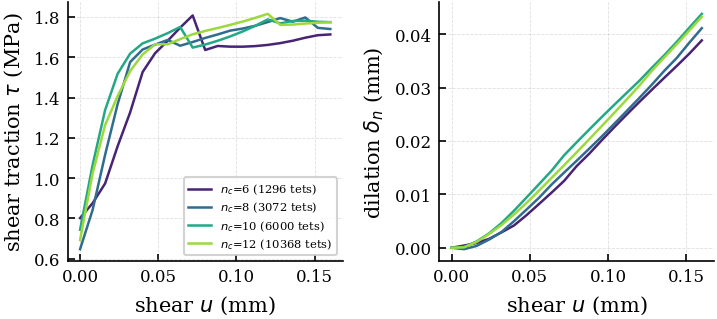
\includegraphics[width=\linewidth]{cv7_traction_history_pub}
\caption{Phase~3 transition-map detection inside the direct-shear loop. Global shear traction $\tau$ and
emergent normal dilation $\delta_n$ as functions of the imposed tangential displacement, with the chart
detector supplying the gap and normal to the FEM. The traces are mesh-converged across the refinement
sequence of Section~\ref{sec:cv7}; the chart-driven response tracks the analytic-surface reference, and
Table~\ref{tab:supp_p3} reports the quantitative agreement.}
\label{fig:supp_traction}
\end{figure}

\subsection{Cyclic loading and the energy ledger}\label{app:supp:p4}

The cyclic study drives the joint through a triangle-wave tangential schedule under constant normal
displacement. It accounts for every term of the first law. The friction model uses a stateful
return-map update, so stick and slip alternate and the shear-traction response forms hysteresis loops.
The Plesha asperity-degradation parameter decays across cycles, from $0.3405$ to $0.3377$ over four
cycles, and the contact Newton residual averages $7\times10^{-5}$. The peak apparent friction is
$\abs{\muapp}\approx0.33$.

% code: rock_joint_decoder_cyclic.py::run_cyclic
The first law states that the external work fed into the joint must reappear as stored energy plus
dissipation. With $\gn<0$ in penetration and slip taken as plastic, the ledger reads
%
\begin{equation}\label{eq:supp_ledger}
W_{\mathrm{ext}}
= \Delta U_{\mathrm{el}}
+ W_{\mathrm{pen}}
+ W_{\mathrm{stick}}
+ W_{\mathrm{fric}},
\end{equation}
%
where each term has a physical meaning. The left side, $W_{\mathrm{ext}}=\sum \fbf_{\mathrm{contact}}\cdot
\mathrm{d}\ubf_{\mathrm{platen}}$, is the machine work the contact tractions do on the moving platen. On
the right, $\Delta U_{\mathrm{el}}=\tfrac12\ubf^{\!\top}\!K\ubf$ is the recoverable strain energy of the
blocks, $W_{\mathrm{pen}}=\tfrac12\sum\varepsilon_n A\,\gn^{2}$ is the recoverable normal penalty energy,
$W_{\mathrm{stick}}$ is the recoverable tangential spring energy of the stuck nodes, and
$W_{\mathrm{fric}}=\sum\abs{\tbf_T}\,\abs{\mathrm{d}\bm{s}_p}\ge0$ is the frictional dissipation
accumulated over the plastic slip increments. The three recoverable terms make up the moving part of the
balance over a cycle: each one returns to its start value once the load closes,
$\Delta U_{\mathrm{el}}\to0$, $W_{\mathrm{pen}}\to0$, $W_{\mathrm{stick}}\to0$. The per-cycle closure
therefore reduces to a single ratio that should equal one,
%
\begin{equation}\label{eq:supp_closure}
\Pi_{\mathrm{cyc}}
= \frac{W_{\mathrm{ext}}}
{\,W_{\mathrm{fric}}+\Delta U_{\mathrm{el}}+W_{\mathrm{pen}}+W_{\mathrm{stick}}\,}
\;\longrightarrow\; 1 .
\end{equation}
%
A value of $\Pi_{\mathrm{cyc}}=1$ means the work in matches the energy out, term for term, over the cycle.

% code: rock_joint_decoder_cyclic.py::energy_report
Measured per cycle, $\Pi_{\mathrm{cyc}}=1.09$ on the first cycle and $1.01$ on the second, the latter
inside the acceptance band $[0.98,1.02]$. The first-cycle excess is the recoverable terms not yet having
returned to zero after a single traversal; by the second cycle they do return, and the ledger closes to
one percent. Figure~\ref{fig:supp_cyclic} shows the hysteresis loops and the per-cycle ledger.

% code: rock_joint_decoder_cyclic.py::energy_report
The \emph{cumulative} ratio over the whole history is a different number, $0.17$, far from one. The
shear-only constant-normal machine work $W_{\mathrm{ext}}$ does not count the dissipation spent seating
the asperities under the initial normal load. The run begins with
$W_{\mathrm{fric}}[0]=0.91$ already accumulated while $W_{\mathrm{ext}}[0]=0$, because the normal-load
seating happens before the tangential schedule starts. That offset enters the denominator of the
cumulative ratio but never the numerator, so it depresses the ratio permanently. The offset is a
bookkeeping artifact, the unmeasured seating dissipation, not an energy violation. The per-cycle balance
of Eq.~\eqref{eq:supp_closure} differences the accumulated work across one full cycle and so cancels the
constant offset; that per-cycle balance is the correct first-law statement, and it closes.

\begin{figure}
\centering
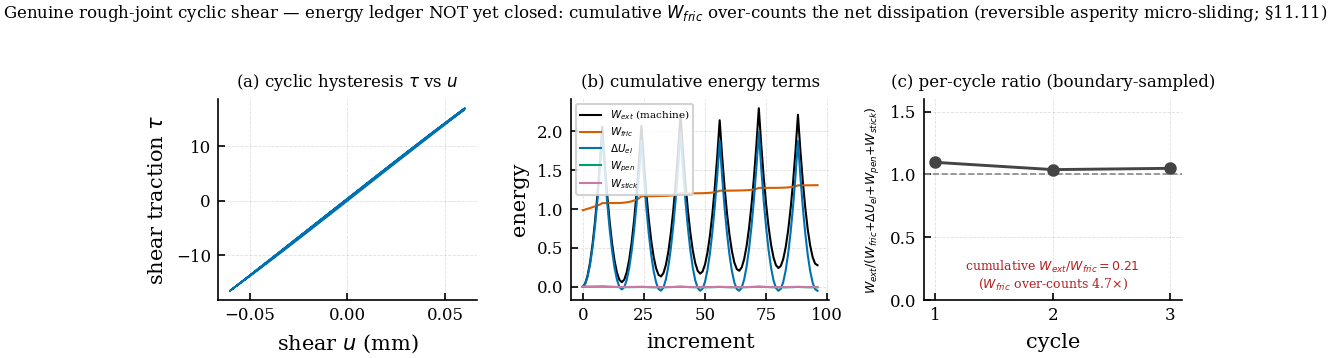
\includegraphics[width=\linewidth]{rock_joint_cyclic_energy_pub}
\caption{Phase~4 cyclic shear under constant normal displacement. Left: stick/slip hysteresis loops of the
shear traction against tangential displacement, with Plesha degradation decaying across cycles. Right: the
energy ledger of Eq.~\eqref{eq:supp_ledger}; the per-cycle closure $\Pi_{\mathrm{cyc}}$ of
Eq.~\eqref{eq:supp_closure} is $1.09$ then $1.01$. The cumulative ratio $0.17$ is the uncounted initial
asperity-seating dissipation, a bookkeeping offset rather than an energy violation.}
\label{fig:supp_cyclic}
\end{figure}

\subsection{Explicit ChartMPM cross-check}\label{app:supp:p5}

% code: rock_joint_mpm_xcheck.py::RoughFloorSDF
The last study checks the frictional response with an independent solver. We discretize a deformable block
with the explicit finite-deformation ChartMPM (linear B-spline transfers, Neo-Hookean response) and shear
it against the \emph{same} band-limited rough surface that the chart-FEM uses, sliding the surface beneath
the block at a constant rate to impose direct-shear kinematics. The contact runs through the existing
per-particle MPM channel: the gap comes from \code{evaluate\_gap}, the normal force from the penalty model,
and the tangential force from regularized Coulomb friction, all scattered as physical-space per-particle
forces through the same projection-to-grid channel as gravity. The solver sees the floor as the analytic
SDF $\phi(\xbf)=z-h(x-u_x,y)$, where $h$ is the rough height field and $u_x$ is the imposed slide.

% code: rock_joint_mpm_xcheck.py::main
The explicit solve reproduced the Coulomb friction floor. A flat-bottomed block sliding on the rough floor
reached an emergent apparent friction $\muapp\approx0.34$ against the prescribed base $\mu=0.4$, within
about $14\%$, and converged stably under dynamic relaxation. This is an independent dynamic confirmation
of the frictional channel that the quasi-static FEM uses.

% code: rock_joint_mpm_xcheck.py::RoughFloorSDF
The explicit solve does not, however, confirm the dilatant interlock. The chart-FEM produces emergent
dilation and an apparent-friction enhancement above the base value because two rough faces ride over one
another. A \emph{mated} rough-on-rough block in the explicit solver, with the full surface in conformal
contact, is unstable in explicit penalty dynamics and diverges without an implicit or mortar contact
treatment. The cross-check therefore validates friction but not dilatancy. We state this limit rather
than hide it: the explicit MPM is a consistent check of the Coulomb response, and the emergent dilatancy
of Section~\ref{sec:cv7} rests instead on the quasi-static implicit chart-FEM, whose consistent tangent
drives the contact Newton residual to $\sim10^{-9}$. An implicit or mortar contact treatment for the
mated MPM case is the documented path to a full dynamic cross-check of dilatancy.

\end{appendix}

\bibliographystyle{unsrtnat}
\bibliography{refs}

\end{document}
